\input{chapters/configuracion.tex}

\begin{document}

%----------------------------------
%Inicio portada
	\begin{titlepage}
\begin{center}
\vspace*{+0.75in}
\textbf{\textsc{\begin{Huge}Cálculo\end{Huge}}}

\vspace*{+0.15in}
\begin{figure}[htb]
\begin{center}
\includegraphics[width=8cm]{../imagenes/complu}\\\ \\\ \\
\textsc{\textbf{\begin{LARGE}Universidad Complutense de Madrid\end{LARGE}}}\\\ \\\ \\\ \\
\textsc{\begin{Large}Facultad de Ciencias Matemáticas\end{Large}}\\\ \\
\textsc{\begin{large}Doble Grado en Matemáticas e Ingeniería Informática\end{large}}
\end{center}
\end{figure}

\vspace*{0.35in}

\textsc{\textbf{\begin{large} Javier Pellejero \end{large}}\\}
Curso 2015-2016
\end{center}
\end{titlepage}
% Fin portada
%-------------------------------------------------------

	\begin{titlepage}
\begin{center}
\vspace*{+0.5in}
\textbf{\textsc{\begin{Huge}Elementos de Ecuaciones\vspace*{+0.1in} Diferenciales Ordinarias\end{Huge}}}

\vspace*{+0.15in}
\begin{figure}[htb]
\begin{center}
\includegraphics[width=8cm]{../imagenes/complu}\\\ \\\ \\
\textsc{\textbf{\begin{LARGE}Universidad Complutense de Madrid\end{LARGE}}}\\\ \\\ \\\ \\
\textsc{\begin{Large}Facultad de Ciencias Matemáticas\end{Large}}\\\ \\
\textsc{\begin{large}Doble Grado en Matemáticas e Ingeniería Informática\end{large}}
\end{center}
\end{figure}

\vspace*{0.25in}

\textsc{\textbf{\begin{large} Javier Pellejero\end{large}}\\}
Curso 2016-2017
\end{center}
\end{titlepage}
\blankpage

\pagenumbering{Roman} % para comenzar la numeracion de paginas en numeros romanos
	\chapter*{}
\begin{flushright}
\textit{Debemos dividir nuestro tiempo entre política y ecuaciones. Pero las ecuaciones son más importantes para mí, porque la política es para el momento actual y una ecuación es para la eternidad}.\\\ \\ Albert Einstein
\end{flushright}

	\chapter*{Prefacio}
	Aquí va el prefacio, evidentemente

	\tableofcontents
	\mainmatter % Empieza a numerar en números arábigos 

	\chapter[Espacios métricos]{Espacios métricos, normados y con producto escalar}
	\section{Espacios métricos}
	
	\begin{defi} 
	 Un espacio m\'etrico $(M,d)$ es un conjunto $M$ con una funci\'on $d \colon M\times M \to \mathbb{R}$ que cumple:
		\begin{enumerate}[1)]
			\item $d(x,y) \geq 0$ $ \forall x, y \in M$
		
			\item $d(x,y) = 0 \Leftrightarrow x = y$
		
			\item $d(x,y) = d(y,x) $ $ \forall x, y \in M$
		
			\item $d(x,y) \leq d(x,z) + d(y,z)$ $    \forall x, y, z \in M$
		\end{enumerate}
	\end{defi}

	\begin{ejem} \ 
		\begin{enumerate}[1)]
			\item En $\R$ con $d(x,y) = |x-y| $ $\forall x, y \in \mathbb{R}$
			\item En $\R ^{n}$ con $d_2(x,y)= \sqrt{\sum_{i = 1}^{n} |x_i-y_i|^{2}} $
			\item En $\R ^{n}$ con $d_1(x,y)= \sum_{i = 1}^{n} |x_i - y_i| $
			\item En $\R ^{n}$ con $d_\infty(x,y)= \underset{1\leq i\leq n}\max|x_i - y_i|$
			\item En $\R^n$ si $p\in (1, +\infty )$ con $d_p(x,y) =(\sum_{i=1}^n |x_i - y_i|)^{1/p}$
			\item En un conjunto arbitrario con
		\[d(x,y)  = \left\{
	       \begin{array}{ll}
		 0      & \mathrm{si\ } x = y \\
		 1 		& \mathrm{si\ } x \neq y \\
	       \end{array}
	     \right.\]
		
			\item En $C\ =\{ f \colon [0,1] \to \mathbb{R}\talque \mathrm{f\ continua\ en\ } [0, 1] \mathrm{con\ } d_\infty(f,g)=\stackbin[{x\in [0,1]}]{}\max |f(x)-g(x)|\}$
			\item Si $M=\{ 0,1\}^n=\{(\theta_1,\theta_2,...\theta_n)\talque\theta_i=1$ \'o $0, \mathrm{\ para\ } 1 \leq i \leq n\} $ con $d((\theta_1...\theta_n),(t_1...t_n))=$ n\'umero de coordenadas distintas.
			\item Sea $(M,d)$ un espacio m\'etrico podemos definir la m\'etrica $p$ que es acotada: $p(x,y)=\\=\dfrac{d(x,y)}{1+d(x,y)} \ \forall x,y \in M$
		\end{enumerate}
	\end{ejem}

		
	\begin{defi}
		 Sea $(M,d)$ un espacio m\'etrico y sea $A \subset M $ definimos el diámetro de $A$ como $\diam(A)=\sup\{d(x,y)\talque x,y \in A\}$
	\end{defi}
	
	\begin{defi}
		Decimos que $A\subset M$ es acotado si tiene di\'ametro finito.\\
	\end{defi}
	
	\begin{ejem} \
		\begin{enumerate}[1)]
			\item $\mathbb{N}$ en $(\mathbb{R},|\cdot|)$ no es acotado.
			\item $\mathbb{N}$ en $(\mathbb{R},\partial)$, siendo $\partial$ la métrica discreta, es acotado.
		\end{enumerate} 
	\end{ejem}
	
	\section{Espacios normados}	
	
	\begin{defi}
		Sea $E$ un espacio vectorial sobre $\mathbb{R}$ una norma en $E$ es una aplicaci\'on \\ $||\cdot||\colon E \to \mathbb{R}$ con las siguienetes propiedades:
		\begin{enumerate}
			\item $\norm{x} \geq 0 \ \forall x \in E$
			\item $\norm{x} = 0 \Leftrightarrow x=0$
			\item $\norm{\lambda x} = |\lambda| \norm{x} \ \forall x\in E, \ \forall \lambda\in E$
			\item $\norm{x+y} \leq \norm{x} + \norm{y} \ \forall x,y \in E$ \textbf{(Desigualdad triangular)}.		
		\end{enumerate}
	\end{defi}
	
	\begin{nota}
	- Un espacio normado $(E,\norm{\cdot})$ es un espacio vectorial junto con la norma $\norm{\cdot}$
	\end{nota}
	
	\begin{ejem} \ 
		\begin{enumerate}[1)]
			\item En $\mathbb{R} ||t||=|t| \ \forall t\in \mathbb{R}$
			\item En $(\mathbb{R}^n,||\cdot||_2)$ donde $||x||_2 =\sqrt{\sum^n_{i=1}x_i^2}\ \forall x \in \mathbb{R}^n$
			\item En $\mathbb{R}^n$ con $||x||_1 =\sum ^n_{i=1}|x_i|$
			\item En $\mathbb{R}^n$ con $||x||_{p_{\ 1<p<+\infty}} =(\sum ^n_{i=1}|x_i|^p)^{1/p}$
			\item En $\mathbb{R}^n$ con $||x||_\infty = \max|x_i|$
			\item En $C([0,1])$ con: 
				\begin{enumerate}[i)]
					\item $||f||_\infty = \max|f(x)| \ \forall f \in C$
					\item $||f||_1 = \int_0^1  |f(x)|dx\ \forall f \in C$
					\item $||f||_2 = \sqrt{\int_0^1  |f(x)|^2dx}\ \forall f \in C$
				\end{enumerate}
		\end{enumerate}		
	\end{ejem}
	
	
	
	\begin{proposicion}
	 Sea $(E,||\cdot||)$ un espacio normado, entonces la aplicación \\
	 $d\colon E\times E \to \mathbb{R}$ definida por $d(x,y)= ||x-y|| \ \forall	x,y \in E$ es una m\'etrica en $E$ \underline{(que llamamos}\\ \underline{ m\'etrica inducida por la norma)}.
	 \end{proposicion}
	
	\section{Espacios vectoriales}	
	
	\begin{defi}
		Sea $E$ un espacio vectorial sobre $\mathbb{R}$, un producto escalar (o producto interno) en $E$ es una aplicaci\'on $\dotproduct{}{}\colon E\times E \to \mathbb{R}$ que cumple:
		\begin{enumerate}[1)]
			\item $\dotproduct{x}{x}\geq 0 \ \forall x\in E$
			\item $<x,x>=0 \Leftrightarrow x=0 \ \forall x \in E$
			\item $<x+y,z>=<x,z>+<y,z> \ \forall x,y,z \in E$
			\item $<\lambda x,y>= \lambda <x,y> \ \forall x,y \in E, \ \forall \lambda \in \mathbb{R}$
			\item $<x,y> = <y,x> \ \forall x,y \in E$
		\end{enumerate}
	\end{defi}
	 
	\begin{ejem} \ 
		\begin{enumerate}[1)]
	 		\item En $\mathbb{R} <t,s>=t\cdot s \ \forall t,s \in \mathbb{R}$
	 		\item En $\mathbb{R}^n <x,y> = \sum^n_{i=1}x_iy_i \ \forall x,y \in \mathbb{R}^n$
	 		\item En $C([0,1]) <f,g>=\int ^1_0 f(x)g(x)dx$
		\end{enumerate}
	\end{ejem}
	
	\begin{corolario} \underline{Consecuencias de la definici\'on}. \\ 
		Si $<,>$ es un producto escalar en un espacio vectorial $E$ se tiene:
		\begin{enumerate}[1)]
			\item $<\lambda x+ \mu y, z>=\lambda <x,z>+\mu <y,z>$
			\item $<x, \lambda y+\mu z> = \lambda <x,y>+\mu <x,z>$
			\item $<x,\lambda y> = \lambda <x,y>$
			\item $<x,0>=<0,x>=0$
		\end{enumerate}
		- $ \forall x,y,z\in E,\ \forall \lambda,\mu \in\mathbb{R}$.
	\end{corolario}
	
	
	\begin{teor}\textbf{Desigualdad de Cauchy - Schwarz.} \\
	Si $<,>$ es un producto escalar en $E$ (sobre $\mathbb{R}$) entonces:
		\begin{align*}
			|<x,y>|\leq \sqrt{<x,x>}\sqrt{<y,y>} \ \forall x,y \in E
		\end{align*}
		\begin{proof}
			Sean $x,y \in E$
			\begin{itemize}
				\item Si $y=0$ \\
		\[\left.
	       \begin{array}{ll}
		 & |<x,y>|=|<x,0>|=0 \\
		 & |<y,y>|=0 
	       \end{array}
	     \right\} \Rightarrow |<x,0>|=\sqrt{<x,x>} \sqrt{0} \] 	
				\item Si $y\neq 0$\\
		Tenemos $<y,y>\ >0$ y $\left(x-\dfrac{<x,y>}{<y,y>} y\right)\in E$ \\
		$0 \leq <x-\dfrac{<x,y>}{<y,y>}y,x-\dfrac{<x,y>}{<y,y>}y>=$ \\
		$= <x,x>-\dfrac{<x,y>}{<y,y>}<x,y> -\dfrac{<x,y>}{<y,y>}<x,y> + \left(\dfrac{<x,y>}{<y,y>}\right)^2<y,y> = $ \\
		$= <x,x> - \dfrac{(<x,y>)^2}{<y,y>} \geq 0 \implies \dfrac{(<x,y>)^2}{<y,y>} \leq <x,x> \implies$ \\
		$\implies(<x,y>)^2\leq <x,x><y,y> \implies |<x,y>|\leq \sqrt{<x,x>}\sqrt{<y,y>}$
			\end{itemize}
		\end{proof}
	\end{teor}	
	
	\begin{observacion}En particular si en $\mathbb{R}^n\ <x,y>=\sum^n_{i=1}x_iy_i$
		\begin{align*}
			\left|\sum^n_{i=1}x_iy_i\right|\leq \sqrt{\sum^n_{i=1}x_i^2}\sqrt{\sum^n_{i=1}y_i^2}
		\end{align*}	
	\end{observacion}
	
	\begin{defi} Si $(E, <,>)$ es un espacio con un producto escalar, definimos en $E$ la norma:
		\begin{align*}
			||x||=\sqrt{<x,x>}
		\end{align*}	
	\end{defi}	
	
	\begin{teor} \textbf{Igualdad del paralelogramo}. \\
		Sea $(E,<,>)$ un espacio vectorial con producto escalar y $||x||=\sqrt{<x,x>}\ \forall x,y\in E$ entonces:
		\begin{align*}
			||x+y||^2+||x-y||^2=2(||x||^2+||y||^2)\ \forall x,y \in E
		\end{align*}	
	\end{teor}
	
	\begin{observacion}No toda norma proviene de un producto escalar, por ejemplo $||\cdot||_\infty$ en $\mathbb{R}^2$
	\end{observacion}

	\begin{proposicion}Sea $E$ un espacio vectorial sobre $\mathbb{R}$ y sea $||\cdot||$ una norma en $E$ entonces $||\cdot||$ proviene de un producto escalar $\iff$ se cumple la igualdad del paralelogramo.
		\begin{proof} \ 
			\begin{itemize}
				\item ($\implies$)  trivial.
				\item ($\impliedby$)  Si definimos $<x,y> = \dfrac{1}{\mu}(||x+y||^2-||x-y||^2)\ \forall x,y 						\in E$ \\
					Se comprueba que $<,>$ es un producto escalar en $E$ y la norma que genera es la 							definida.
			\end{itemize}
		\end{proof}
	\end{proposicion} %Espacios métricos, normados y con producto escalar
	\chapter{Topología de Espacios métricos}
	\section{Conjuntos abiertos y cerrados}
	\begin{nota}
		Sea $(M,d)$ un espacio m\'etrico recordamos que si $N\subset M$ entonces $(N,d|_{_{N\times N}})$ es un espacio m\'etrico.
	\end{nota}
	
	\begin{defi} Sea $a\in M $ y $r>0$
		\begin{itemize}
			\item $B(a,r)= \{ x\in M\talque d(x,a)<r\}$ \underline{Bola abierta de centro $a$ y radio 				$r$.}
			\item $\overline{B}(a,r)=\{ x\in M\talque d(x,a)\leq r\}$ \underline{Bola cerrada de centro $a$ y radio $r$.}
		\end{itemize}
	\end{defi}
	
	\begin{defi} Sea $(M,d)$ y sea $A \subset M$ decimos que:
		\begin{itemize}
			\item \underline{$A$ es abierto} si $\forall a \in A \ \exists r>0\talque B(a,r) \subset A$
			\item \underline{$A$ es cerrado} si $A^c(=M\setminus A)$ es abierto.
			\item Sea $a\in M$, decimos que \underline{$U\subset M$ es entorno de $a$} si $\exists r>0\ | 				\ B(a,r) \subset U$
		\end{itemize}
	\end{defi}
	
	\begin{proposicion}
		$A$ es abierto $\iff \ A$ es entorno de $a,\ \forall a \in A$
	\end{proposicion}
	
	\begin{proposicion}Propiedades de los subconjuntos abiertos de $M$
		\begin{enumerate}[1)]
 			\item $M,\ \emptyset$ Son abiertos.
 			\item La uni\'on de abiertos es abierta.
 			\item La intersecci\'on de una familia \underline{finita} de abiertos es un subconjunto 						abierto.
		\end{enumerate}
	\end{proposicion}

	\begin{corolario} Por las leyes de Morgan obtenemos las siguientes propiedades de subconjuntos cerrados de $M$:
 		\begin{enumerate}[1)]
			\item $M,\ \emptyset$ Son cerrados.
			\item La intersecci\'on de cerrados es cerrada.
			\item La uni\'on de una familia \underline{finita} de cerrados es un subconjunto cerrado.\\
	 	\end{enumerate}
 	\end{corolario}
 	
 	\section{Topología básica}
 	
 	\begin{defi} Sea $A\subset M$ y sea $x\in M$
		\begin{itemize}
			\item Decimos que $x$ es \underline{punto interior} de $A$ si $\exists r>0\talque B(x,r)\subset A$
			\item Decimos que $x$ es \underline{punto de acumulaci\'on} de $A$ si $\forall r>0\talque (B(x,r)-\{ x\}\cap A) \neq \emptyset$
			\item Decimos que $x$ es \underline{punto adherente} de $A$ si $\forall r>0\talque B(x,r)\cap A \neq \emptyset$
			\item Decimos que $x$ es \underline{punto frontera} de $A$ si \[\forall r>0\
\left\{
	      	\begin{array}{ll}
		 B(x,r)\cap A \neq \emptyset \\
		 B(x,r)\cap A^c \neq \emptyset \\
	       \end{array}
	     \right.\]
	    	\item Decimos que $x$ es \underline{punto aislado} de $A$ si $\exists r>0\talque B(x,r)\cap A = \{x\}$		
			\item Decimos que $x$ es \underline{punto exterior} de $A$ si $\exists r>0\talque B(x,r)\subset A^c$
		\end{itemize}
	
		\begin{enumerate}[-]
			\item $\mathring{A}=$ puntos interiores de $A$
			\item $A'=$ puntos de acumulaci\'on de $A$
			\item $\overline{A}=$ puntos adherentes de $A$
			\item $\fr(A)=$ puntos frontera de $A$
			\item $\ais(A)=$ puntos aislados de $A$
		\end{enumerate}
	\end{defi}	
	
	\begin{proposicion}\ 
		\begin{enumerate}[1)]
			\item $\mathring{A}$ es el mayor abierto contenido en $A$ 
				\begin{align*}
					\mathring{A} =\cup\{ G \subset M\talque G \mathrm{\ es\ abierto\ y\ } G\subset A\}
				\end{align*}
			\item $\overline A$ es el menor cerrado que contiene a $A$
				\begin{align*}
					\overline A=\cap\{F\subset M\talque F \mathrm{\ es\ cerrado\ y\ } A\subset F\}
				\end{align*}
		\end{enumerate}
	\end{proposicion}
	
	\begin{proposicion} \ 
		\begin{itemize}
			\item $A$ es abierto $\iff A = \mathring{A}$
			\item $A$ es cerrado $\iff A =\overline{A}$ \\
		\end{itemize}
	\end{proposicion}
	
	\begin{nota}Ser ``abierto'' o ``cerrado'' dependen del espacio ambiente.
		\begin{ejem} $(0,1]$ es cerrado en $\mathbb{R}^+$ y no lo es en $\mathbb{R}$\\
		\end{ejem}
	\end{nota}
	
	\begin{proposicion} \ 
		\begin{itemize}
			\item $\overline{A}= A\cup \fr(A)=A\cup A'=\ais(A)\cup A'$
			\item $\fr(A)=\overline{A}\setminus\mathring{A}$
		\end{itemize}
	\end{proposicion}	
	
	\begin{defi}Una m\'etrica $d$ en un conjunto $M$ genera una topolog\'ia que es la colecci\'on de los conjuntos abiertos. La denotamos as\'i:
	\[\tau_d=\{A\subset M\talque A \mathrm{\ es\ abierto}\}\]
	\end{defi}
	
	\begin{defi} Sean $d_1$ y $d_2$ m\'etricas en un conjunto $M$, diremos que son 				 					\underline{equivalentes} si generan la misma topolog\'ia; es decir:
		\[\tau_{d_1}=\tau_{d_2}\]
	\end{defi}
	
	\begin{proposicion} Sean $d_1$ y $d_2$ m\'etricas en $M$, $d_1 \equiv d_2 \iff \ \forall x\in M, \ \forall r>0 \\ \exists\gamma_1>0\talque B_{d_1}(x,\gamma_1)\subset B_{d_2}(x,r)$ y $ \exists\gamma_2>0\talque B_{d_2}(x,\gamma_2)\subset B_{d_1}(x,r)$\\
	
	- Una condici\'on suficiente para que dos m\'etricas $d_1$ y $d_2$ en $M$ sean equivalentes es que $\exists c,C>0$ de manera que:
	\[cd_1(x,y)\leq d_2(x,y)\leq Cd_1(x,y)\ \forall x,y\in M\implies d_1\equiv d_2\] \\
	\underline{-Sin embargo esta condici\'on no es necesaria generalmente}\\
	-Si la m\'etricas $d_1$ y $d_2$ provienen de una norma, esta condici\'on se hace entonces \underline{necesaria} adem\'as de suficiente para que dichas m\'etricas sean equivalentes; es decir:
	\[\mathrm{Si\ }d_1,d_2\mathrm{\ provienen\ de\ una\ norma:\ }\]
	\[d_1\equiv d_2\iff \exists c,C>0 \talque cd_1(x,y)\leq d_2(x,y)\leq Cd_1(x,y)\ \forall x,y\in M\]
	\end{proposicion}	
	
	\begin{defi} Decimos que \underline{dos normas son equivalentes} en un espacio $E$ si $||\cdot||$ y $||\cdot||'$ generan la misma topolog\'ia.
	\end{defi}
	
	\begin{proposicion} $||\cdot||$ y $||\cdot||'$ son equivalentes $\iff \exists m,M>0$ tal que\\
	$m||x||\leq||x||'\leq M||x||\ \forall x\in E$
	\end{proposicion}
	\newpage
	\begin{ejem}
		En $(\mathbb{R}^2,d_2)$, sea $A=\{(x,y)\in \mathbb{R}^2\talque x>0,y>0,xy>1\}$ $A$ es abierto?\\
		
		En efecto $A$ es abierto:
		\begin{proof}		
			Probaremos que $\forall(a,b)\in A,\ \exists r>0\talque B((a,b),r)\subset A$
			\[\mathrm{Sabemos\ }  \left\{
				\begin{array}{ll}
					a>0 \\
			 		b>0 \\
					ab>1\\
		       \end{array}
		    \right\}\]
			\[\mathrm{Supongamos\ que\ }(x,y)\in B((a,b),r)\implies\{\sqrt{(x-a)^2+(y-b)^2}=d((x,y),(a,b))\}\implies \] \\
	\[\implies \left\{
	       \begin{array}{ll}
		 |x-a|<r \\
		 |y-b|<r \\
	       \end{array}
	     \right\}\implies \left\{
	       \begin{array}{ll}
		 a-r<x<a+r \\
		 b-r<y<b+r \\
	       \end{array}
	     \right\}\implies xy>(a-r)(b-r)=\] \\
	     \[=ab-r(a+b)+r^2>ab-r(a+b)\geq 1\iff ab-1\geq r(a+b)\iff\dfrac{ab-1}{a+b}\geq r>0\]
	     \[\mathrm{Por\ tanto\ para\ }0<r\leq \dfrac{ab-1}{a+b},\ xy>1.\mathrm{\ Veamos\ por\ ultimo\ que\ }x,y>0\]
	     \[ x>a-r\geq a-\dfrac{ab-1}{a+b}=\dfrac{a(a+b)-ab+1}{a+b}=\dfrac{a^2+1}{a+b}>0 \]
		 \[y>b-r\geq b-\dfrac{ab-1}{a+b}=\dfrac{b(a+b)-ab+1}{a+b}=\dfrac{b^2+1}{a+b}>0 \]
		\end{proof}
		\begin{figura}\ \\
	\begin{center}
	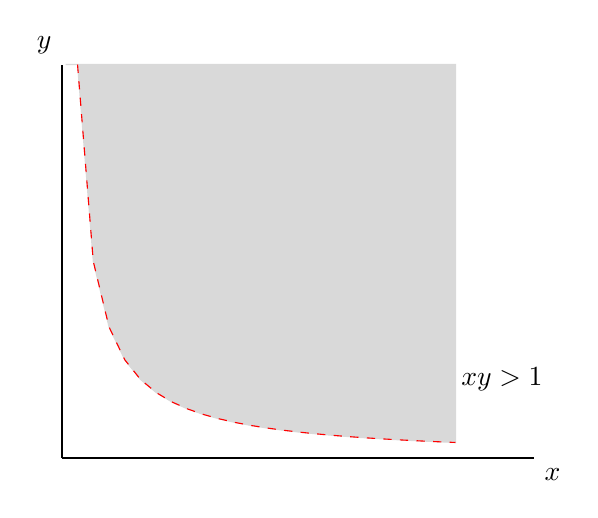
\begin{tikzpicture}
	\fill (4.95,1) circle (0.5pt)node[anchor=west] {$xy>1$};
	\filldraw[gray!30] plot [domain=0.05:5] ({\x},{5})
-- plot [domain=5:0.2] ({\x},{1/\x})
-- cycle;
		\draw[thick](0,0) -- (6,0) node[anchor=north west] {$x$};
		\draw[thick] (0,0) -- (0,5) node[anchor=south east] {$y$};
		\draw[domain=0.2:5,variable=\x,red,dashed] plot ({\x},{1/\x});
	\end{tikzpicture}
	\end{center}
	\end{figura}
	\end{ejem} %Topología de Espacios métricos
	\chapter{Congruencia en Espacios métricos}
	\section{Sucesiones, sucesiones de Cauchy y espacios métricos completos}
	     
	\begin{defi} Sea $(M,d)$ un espacio m\'etrico:\\
	     Sea $\sucesion{x}{n}$ una sucesi\'on en $M$, y sea $x\in M$, diremos que $\sucesion{x}{n}$ converge a $x$ si \\
	     $\forall \varepsilon>0\ \exists k\in \N\talque d(x_n,x)<\varepsilon\ \forall n\geq k$\\
	     Si es así denotamos a $x$ \underline{l\'imite de la sucesi\'on}. Y lo denotamos $\limite{x_n}{\ntiende}$ \'o $x_n\xrightarrow{n\rightarrow \infty}x$.
	\end{defi}
	     
	\begin{proposicion}
     	Si el l\'imite de una funci\'on existe, este es \'unico.
     \end{proposicion}
	     
     \begin{defi} Diremos que $\sucesion{x}{n}$ \underline{converge} si tiene l\'imite. En caso contrario diremos que \underline{diverge}.
     \end{defi}
	     
     \begin{observacion} Si $d$ y $d'$ son m\'etricas equivalentes en $M$ y $\sucesion{x}{n}$ es sucesi\'on en $M$, entonces:\\
	     \[\sucesion{x}{n}\mathrm{\ converge\ en\ }(M,d)\iff \sucesion{x}{n} \mathrm{\ converge\ en\ }(M,d')\]
     \end{observacion}
	
	\begin{ejem} \
		\begin{itemize}
		\item $\mathrm{En\ }(\R,d_2):\ \sucesionelement{c}{n}\mathrm{\  con\ }c\in \mathbb{R},\ \sucesionelement{\dfrac{1}{n}}{n},\ \sucesionelement{\left(1+\dfrac{1}{n}\right)^n}{n}$
\item  $\mathrm{En\ }(\mathbb{R}^2,d_2):\ \sucesionelement{\dfrac{1}{n},\left(1+\dfrac{1}{n}\right)^n}{n}\ \mathrm{(que\ converge\ a\ }(0,e)).$
		\end{itemize}
    \end{ejem}
	    
    \begin{proposicion}Sea $(M,d)$ espacio m\'etrico, $A\subset M$ y $x\in M$, se cumple:
   		\begin{enumerate}[1)]
    		\item $x\in A'\iff \exists \sucesion{x}{n} \talque \ x_n\in A-\{x\}\ \forall n\in \N$, convergente a $x$.
    		\item $x\in\overline{A}\iff \exists\sucesion{x}{n}\talque x_n\in A\ \forall n\in \N$ convergente a $x$.
    		\item $x\in Fr(A)\iff \exists \sucesion{x}{n}\talque x_n\in A\ \forall n\in \mathbb{N}$ y $\exists \sucesion{y}{n}\talque y_n\in A^c\ \forall n\in \mathbb{N}$, convergentes a $x$.
    		\item $A$ es cerrado $\iff \forall a'\in A', a'\in A\iff \forall \sucesion{x}{n}\talque x_n\in A\ \forall n\in \mathbb{N}$, convergente, cumple que: $\limite{x_n\in A}{n\rightarrow \infty} $
    	\end{enumerate}
    \end{proposicion}
	    
    \begin{defi}. Sea $(M,d)$ espacio m\'etrico y $\sucesion{x}{n}$ una sucesi\'on en $M$, decimos que $\sucesion{x}{n}$ \underline{es de Cauchy} si $\forall\varepsilon>0\ \exists k\in \mathbb{N}\talque d(x_p,x_q)<\varepsilon\ \forall p,q \geq k$.
    \end{defi}
	    
    \begin{proposicion}. Sea $(M,d)$ un espacio m\'etrico:
    	\begin{enumerate}[i)]
    		\item Sea $\sucesion{x}{n}$ convergente $\ximplies{(\nimpliedby)}{} \sucesion{x}{n}$ es sucesi\'on de Cauchy.
    		\item Sea $\sucesion{x}{n}$ sucesi\'on de Cauchy $\ximplies{(\nimpliedby)}{} \sucesion{x}{n}$ es acotada.
    	\end{enumerate}
    \end{proposicion}
	    
	\begin{observacion}Veamos, en efecto, que las anteriores propiedades no son equivalentes.
	    \begin{itemize}
	    		\item Una sucesi\'on de Cauchy no tiene por qu\'e converger; es el caso de $\sucesionelement{\left(1+\dfrac{1}{n}\right)^n}{n}$ es una sucesi\'on de Cauchy en $(\Q,|\cdot|)$ pero no converge.
	    		\item $\sucesion{x}{n}$ acotada$ \nimplies \sucesion{x}{n}$ es de Cauchy; Por ejemplo: $\sucesionelement{(-1)^n}{n}$
	    \end{itemize}
	\end{observacion}
	    
	\begin{defi} Un espacio m\'etrico \underline{es completo} si toda sucesi\'on de Cauchy es convergente.
	\end{defi}   
	    
	\begin{ejem} \
	    \begin{itemize}
	    		\item Completos: $(\mathbb{R},|\cdot|),\ (\mathbb{R}^2,d_1),\ (\mathbb{N},|\cdot|)$.
	    		\item No completos: $(\mathbb{Q},|\cdot|), \ (\mathbb{R}\setminus\mathbb{Q},|\cdot|),\ (\mathbb{R}\setminus\{0\},|\cdot|)$.
	    \end{itemize}
	\end{ejem}
	    
	\begin{defi}Si $\sucesion{x}{n}$ es una sucesi\'on y $\sucesion{n}{k}$ es una sucesi\'on estrictamente creciente en $\mathbb{N}$ decimos que $\sucesionelement{x_{n_k}}{k}=\{x_{n_1},x_{n_2},x_{n_3}...\}$ \underline{ es una subsucesi\'on} de $\sucesion{x}{n}$.
	\end{defi}
	    
	\begin{proposicion}. Sea $(M,d)$ espacio m\'etrico y sea $\sucesion{x}{n}$ una sucesi\'on en $M$ que converge a $x$, entonces cualquier subsucesi\'on de $\sucesion{x}{n}$ converge tambi\'en a $x$.
		\begin{proof} \ \\
			Sea $\sucesionelement{x_{n_k}}{k}$ subsucesi\'on de $\sucesion{x}{n}$, comprobemos que $x_{n_k}\xrightarrow{k\rightarrow\infty}x$\\
	    Dado $\varepsilon>0$, como $x_n\xrightarrow{k\rightarrow\infty}x,\ \exists n_0\in \mathbb{N}\ \talque\ d(x_n,x)<\varepsilon\ \forall n\geq n_0$. Ahora, si $k\geq n_0$ entonces $n_k\geq n_{n_0}\geq n_0$. Luego $d(x_{n_k},x)<\varepsilon$
		\end{proof}
	\end{proposicion}
	
	\begin{corolario}\ 
	    \begin{enumerate}[1)]
	    		\item Si una sucesi\'on tiene dos subsucesiones que convergen a distinto l\'imite, entonces la sucesi\'on diverge.
	    		\item Sean $d$ y $d'$ m\'etrcias equivalentes en $M$:
	    		\[\sucesion{x}{n}\mathrm{\ converge\ en\ }(M,d)\iff \sucesion{x}{n}\mathrm{\ converge\ en\ }(M,d')\]
	    \end{enumerate}
	\end{corolario}
	    
	\begin{nota} En general $(M,d)$ y $(M,d')$ NO tienen las mismas sucesiones de Cauchy.
	\end{nota}
	    
	\begin{ejem}Sean $(\mathbb{R},|\cdot|)$ y $(\mathbb{R},d)$ siendo $d(x,y)=|arctg(x)-arctg(y)|$ son equivalentes pero no tienen las mismas sucesiones de Cauchy.
	\end{ejem}
	    
	\begin{proposicion}. Si $d$ y $d'$ provienen de una misma norma, entonces $(M,d)$ y $(M,d')$ tienen las mismas sucesiones de Cauchy.
	    \begin{proof}
	    	Por provenir $d$ y $d'$ de una misma norma, $\exists\alpha,\beta>0$ tal que $\alpha d(x,y)\leq d'(x,y)\leq \beta d(x,y)\ \forall x,y\in M$
	    \end{proof}
	\end{proposicion}
	    
	\section{Compacidad de conjuntos}	    
	 
	\begin{defi}. Sea $(M,d)$ espacio m\'etrico y $A\subset M$. Entonces definimos un recubrimiento de $A$ como \underline{la familia} $\{G_\alpha:\alpha\in\Gamma\}$ \underline{de conjuntos abiertos} tal que: \[\cup_{\alpha\in\Gamma}G_\alpha\supset K\]
	\end{defi}
	    
	\begin{defi}. Sea $(M,d)$ un espacio m\'etrico y sea $K\subset M$, diremos que \underline{$K$ es compacto} si todo recubrimiento abierto de $K$ posee un subrecubrimiento finito; es decir, para cada familia $\{G_\alpha,\alpha\in\Gamma\}$ de conjuntos abiertos tal que $\cup_{\alpha\in\Gamma}G_\alpha\supset K,\ \exists\sigma\subset\Gamma, \sigma$ finito, tal que: \[\cup_{\alpha\in\sigma}G_\alpha\supset K\]
	\end{defi}
	    
	\begin{ejem} Ejemplos de conjuntos compactos:
		\begin{itemize}
	  		\item Cualquier conjunto finito.
	  		\item Sea $\sucesion{x}{n}$ convergente en $M$ a $x_0$, entonces $\{ x_0\}\cup\{ x_n\talque n\in \mathbb{N}	\}$ es compacto.
		\end{itemize}
	\end{ejem}
	  
	\begin{proposicion} \underline{Propiedades de los compactos}.\\
	Sea $(M,d)$ espacio m\'etrico y $K\subset M$:\\
	  -$K$ es compacto en $(M,d)\iff K$ es compacto en $(K,d|_{K\times K})$.
		\begin{enumerate}[1)]
			\item Si $K$ es compacto $\implies K$ es cerrado y acotado.
	  			\begin{proof}\
	  				\begin{itemize}
	  					\item Veamos primero que compacto$\implies$ acotado.\\
	  			Sea $M\neq\emptyset$, sea $a\in M$ como $M=\cup^\infty_{n=1} B(a,n)$\\
	  			As\'i $\{B(a,n)\talque n\in \mathbb{N}\}$ es un recubrimiento por abiertos de $K$, y por ser $K$ compacto $\exists	n_1,n_2,...n_k\talque K\subset\cup^k_{i=1}B(a,n_i)=B(a,m)$ con $m=max\{n_1,...n_k\},$ por tanto $K$ es acotado.
	  					\item Veamos ahora que compacto$\implies$ cerrado.\\
	  			Veamos que $K^c$ es abierto. Sea $b\in K^c\ \forall x\in K,$ como $x\neq b,\ \exists r_x>0\talque B(x,r_x)\cap B(b,r_x)=\emptyset.$\\
	  			Entonces $\{B(x,r_x)\talque x\in K\}$ es un recubrimiento de abiertos tal que $\cup_{x\in K}B(x,r_x)\supset K$. Luego por ser $K$ compacto $\exists x_1,x_2,...x_m\in K\talque K\subset\cup^m_{i=1}B(x_i,r_{x_i})$.\\
	  			Tomemos $r=min\{r_{x_1},r_{x_2},...r_{x_m}\}$, tenemos que $B(b,r)\subset K^c$ ya que $(B(b,r)\cap K)\subset (B(b,r)\cap(\cup^m_{i=1}B(x_i,r_{x_i})))=\cup^m_{i=1}(B(b,r)\cap B(x_i,r_{x_i}))\subset\cup^m_{i=1}(B(b,r_{x_i})\cap B(x_i,r_{x_i}))=\emptyset\implies K$ es cerrado. $_\Box$
	  				\end{itemize}
				\end{proof}
	  		\item Si $K\subset M$ es compacto, entonces $K$ es \underline{precompacto} (también llamado "totalmente acotado"), si $\forall\varepsilon >0\ \exists x_1,x_2...x_n\in K\talque K\subset \bigcup^n_{i=1} B(x_i,\varepsilon)$
	  			\begin{proof} Dado $\varepsilon>0$, basta tener en cuenta que $\{B(x,r)\talque x\in K\}$ es recubrimiento por abiertos de $K$ por ser $K$ compacto posee un subrecubrimiento finito.
	  			\end{proof}
	  		\item Sea $K$ compacto $\subset M$  y sea $C\subset K \talque C$ es cerrado$\implies C$ es compacto.
	  			\begin{proof}
	  			Sea $\{G_\alpha :\alpha \in \Gamma\}$ una familia de abiertos en $M \talque \\ \cup_{\alpha\in\Gamma} G_\alpha \supset C$ \\
	  			Como $C$ es cerrado, entonces $C^c$ es abierto y $M\supset K=C^c \cup (\cup_{\alpha\in\Gamma} G_\alpha)$. Así $\{C^c\}\cup\{G_\alpha :\alpha\in\Gamma\}$ es un recubrimiento por abiertos de $K$. Como $K$ es compacto $\exists \alpha_1,\alpha_2 ...\alpha_k \in\Gamma\talque K\subset C^c\cup(\cup^k_{i=1}G_{\alpha_i})$\\
	  			Entonces, como $C\subset K$, tenemos $C\subset\cup^k_{i=1}G_{\alpha_i} \implies C$ es compacto.
	  			\end{proof}
		\end{enumerate}
	\end{proposicion}
	
	\begin{proposicion} En $\R^n$ con la métrica usual, sea $A\subset \R^n$, entonces $A$ es acotado $\iff$ $A$ es precompacto.
	\begin{observacion} En otros espacios métricos, en general, no es cierta la proposición:\\
	\underline{Ejemplo}: En $\R$ con la métrica discreta, $(0,1)$ es acotado pero no precompacto. Sea $\varepsilon_0=0,5$ entonces $(0,1)=\stackbin[x\in(0,1)]{}\bigcup B(x,\varepsilon)$ y en $(0,1)$ hay infinitos puntos.
	\end{observacion}
	\end{proposicion}
	
	\begin{teor} \textbf{Teorema de Bolzano-Weierstrass}\\
		Sea $(M,d)$ espacio métrico y sea $K\subset M$, entonces son equivalentes:
			\begin{enumerate}[(a)]
				\item $K$ compacto.
					\[\iff\]
				\item Todo subconjunto infinito de $K$ posee un punto de acumulación contenido en $K$
					\[\iff\]
				\item Toda sucesión en $K$ posee una subsucesión convergente a un elemento de $K$
			\end{enumerate}
		\begin{proof}\ 
			\begin{itemize}
				\item $(1)\implies(2)$\\
					Sea $K$ compacto. Sea $S\subset K$, $S$ infinito, probemos que $\exists x\in S'\cap K$\\
	Supongamos que no, que no hay ningún punto de $K$ que pertenezca a $S'$\\
	Entonces $\forall x\in K\ \exists\gamma_x>0\talque (B(x,\gamma_x)\setminus\{x\})\cap S=\emptyset\ (*)$\\
	Tenemos que $\{B(x,\gamma_x)\talque x\in K)$ es un recubrimiento por abiertos de $K$ y por ser $K$ compacto $\exists x_1,x_1...x_m\in K\talque K\subset\cup^m_{i=1}B(x_i,\gamma{x_i})$. Como $S\subset K$, tenemos $S\subset \cup^m_{i=1}B(x_i,\gamma{x_i})$\\
	Por $(*)\ S\subset\{x_1,x_2...x_m\}$ y esto es absurdo pues $S$ es infinito. Por tanto existe $x_0 \in K\talque x_0\in S'$
				\item $(2)\implies(3)$\\
	Sea $\{x_n\}^\infty_{n=1}$ sucesión en $K$, veamos que tiene una subsucesión convergente.
	Entonces, sea $S$ el rango de $\{x_n\}^\infty_{n=1}$, es decir, $S=\{x_n\talque n\in\N\}$. Si:
					\begin{itemize}
						\item $S$ finito. Existe un elemento que se repite infinitas veces y por tanto existe una subsucesión constante y por tanto convergente en un elemento de $K$
						\item $S$ infinito $\implies$ por (2), $\exists x_0\in S'\cap K$. Construyamos la subsucesión:\\
	Como $x_0\in S'\ \forall \varepsilon>0 (B(x_0,\varepsilon)\setminus\{x_0\})\cap S \neq\emptyset\implies$ la intersección $B(x_0,\varepsilon)\cap S$ es infinita.					
	Así, $(B(x_0,1)\setminus\{x_0\})\cap S\neq\emptyset\implies \exists n_1\in\N \talque x_{n_1}\in B(x_0,1)$\\
	Como $(B(x_0, 1/2)\setminus\{x_0\})\cap S$ es infinito $\implies \exists n_2>n_1 \talque x_{n_2}\in B(x_0,1/2)$\\
	...\\
	\ \ \ $(B(x_0, 1/k)\setminus\{x_0\})\cap S$ es infinito $\implies \exists n_k>n_{k-1} \talque x_{n_k}\in B(x_0,1/k)$. Y por tanto $\exists\{n_k\}^\infty_{k=1} \subset\N$ y creciente$\talque x_{n_k} \in B(x_0,1/k)\ \forall k\in\N$. Es claro que $\{n_k\}^\infty_{k=1}$ es subsucesión de $\{x_n\}$ y como $0<d(x_0,x_{n_k})\leq 1/k\ \forall k\in\N$, tenemos que \\
	$d(x_{n_k},x_0)\xrightarrow{k\rightarrow\infty}0 \iff x_{n_k}\xrightarrow{k\rightarrow\infty}x_0$
					\end{itemize}
				\item $(3)\implies(1)$ \\
	Veamos primero que $K$ es precompacto.\\
	Supongamos que no. Si $K$ no es precompacto $\implies \exists \varepsilon_0>0\talque K$ no está contenido en la unión de un número finito de bolas centradas en puntos de $K$ y radio $\varepsilon_0$\\
	Sea $x_1\in K$. Como $K\not\subset B(x_1,\varepsilon_0)\implies \exists x_2\in K\setminus B(x_1,\varepsilon_0)$\\
	\ \ \ $K\not\subset (B(x_1,\varepsilon_0)\cup B(x_2,\varepsilon_0))\implies\exists x_3\in K\setminus (B(x_1,\varepsilon_0)\cup B(x_2,\varepsilon_0))$\\
	\ \ \ ...\\
	Obtenemos $\{x_n\}^\infty_{n=1}\subset K \talque \forall n\in\N x_{n+1}\in K\setminus(\cup^n_{i=1}B(x_i,\varepsilon_0))\implies \{x_n\}$ no es de Cauchy pues $d(x_n,x_m) \geq \varepsilon_0\ \forall n,m; n\neq m.$ Es más, de aquí podemos deducir que ninguna subsucesión de $\{x_n\}$ es de Cauchy $\implies$ ninguna convergente$\implies$ contradice (3)\\
	Por lo tanto ya sabemos que $K$ es precompacto. Veamos ahora que es compacto:\\
	Sea $\{G_\alpha\ | \alpha\in\Gamma\}$ recubrimiento por abiertos de $K$. Veamos que\\
	 $\exists r>0\talque \forall x\in K\ \exists \alpha_x\in\Gamma \talque B(x,r)\subset G_{\alpha_x}$:\\
	 Si no, $\forall\varepsilon>0\ \exists x_\varepsilon\in K\talque B(x_\varepsilon,\varepsilon) \nsubset G_\alpha\ \forall\alpha\in\Gamma$\\
	 Luego, $\forall n\in\N\ \exists x_n\in K\talque B(x_n,\dfrac{1}{n})\nsubset G_\alpha\ \forall\alpha\in\Gamma$\\
	 Tenemos así $\{x_n\}$ sucesión en $K$ y por la hipótesis (3) $\exists \{x_{n_j}\}^\infty_{j=1}$ subsucesión$\talque x_{n_j} \xrightarrow [j\rightarrow\infty]{}x_0\in K$\\
	 Como $x_0\in K \subset\cup_{\alpha\in\Gamma}G_\alpha\ \exists \alpha_0\in\Gamma \talque x_0\in G_{\alpha_0}$. Como  este es abierto, $\exists \delta>0\talque B(x_0,\delta)\subset G_{\alpha_0}.$ Como $x_{n_j} 
	 \xrightarrow[j\rightarrow\infty]{}x_0$ y $\dfrac{1}{n_j}\xrightarrow[j\rightarrow\infty]{}0$; para 
	 $\dfrac{\delta}{2}>0,\ \exists m\in\N\talque d(x_{n_m},x_0)<\dfrac{\delta}{2}$
	  y $\dfrac{1}{n_m}<\dfrac{\delta}{2}$.\\
	 Entonces $B(x_{n_m},\dfrac{1}{n_m})\subset B(x_0,\delta)$ con lo que llegamos a una contradicción.\\	 
	 Visto ahora que $\exists r>0\talque\forall x\in K\ \exists \alpha_x\in\Gamma\talque B(x,r)\subset G_{\alpha_x}$ y sabiendo que es precompacto:\\
	 $K$ precompacto $\implies \exists y_1,...,y_m\in K\talque K\subset\cup^m_{i=1}B(y_i,r)\subset \cup^m_{i=1}G_{\alpha_{y_i}}\implies$hemos extraído un subrecubrimiento finito.
					
			\end{itemize}
		\end{proof}
	\end{teor}
	
	\begin{proposicion} Consecuencia del teorema.\\
		Si $K$ es compacto$\implies K$ es completo.
	\end{proposicion}
			
	\begin{proposicion}
		Si $K$ es compacto$\implies K$ es precompacto.
	\end{proposicion}
	
	\begin{teor}\underline{Teorema de Heine Borel}.\\
		Sea $n\in\N$, $(\R^n,d_2)$ espacio métrico y sea $A\subset \R^n$ compacto $\iff A$ es cerrado y acotado.
		\begin{proof}
		\ 
			\begin{itemize}
				\item $``\implies$'' Se cumple para todo espacio métrico.
				\item $``\impliedby$'' Supongamos que $A\subset\R^n$ es cerrado y acotado. Probemos que $A$ es compacto. Por \textit{Bolzano-Weierstrass} basta probar que toda sucesión en $A$ posee una subsucesión convergente a un elemento de $A$.\\
	Sea $\sucesion{x}{k}=\{(x_1^k,x_2^k,...,x_n^k)\}^\infty_{k=1}$ una sucesión en $A$, como $A$ es acotado, entonces $\sucesion{x}{k}$ es acotado en $\R^n$. Así cada sucesión $\{x_i^k\}_{k=1}^\infty;$\\
	$1\leq i\leq n,$ es acotada en $\R$. Como $\{x_1^k\}_{k=1}^\infty$ es acotada, $\exists\sigma_1\colon \N\to\N$ estrictamente creciente $\talque \{x_1^{\sigma_1 (k)}\}^\infty_{k=1}$ converge.\\
	Como $\{x_2^{\sigma_1 (k)}\}_{k=1}^\infty$ es acotada, $\exists\sigma_2\colon \N\to\N$ estrictamente creciente $\talque \{x_2^{\sigma_2 (k)}\}^\infty_{k=1}$ converge. Repitiendo esto $n$-veces , tenemos que  $\exists\sigma_n\colon \N\to\N$ estrictamente creciente $\talque \{x_n^{\sigma_n (k)}\}^\infty_{k=1}$ converge y también $\{x_i^{\sigma_n (k)}\}^\infty_{k=1}$ con $1\leq i\leq n, \implies$ Sea $x_i=\lim_{k\rightarrow\infty} x_i^{\sigma_n(k)}$ y tenemos que         $\{x^{\sigma_n(k)}\}^\infty_{k=1}$ subsucesión que converge a $(x_1, x_2,...,x_n)$\\
	Como $x^{\sigma_n(k)} \in A,\ \forall k \in \N$ entonces $x^{\sigma_n(k)}\xrightarrow[k\rightarrow\infty]{}(x_1,x_2,...,x_n)$; y ahora, como $A$ es cerrado $(x_1,x_2,...,x_n)\in A$
			\end{itemize}
		\end{proof}
	\end{teor}
	
 %Congruencia en Espacios métricos
	\chapter{Conjuntos conexos en espacios métricos}
	\section{Conjuntos conexos}
	\begin{defi}
		Sea $(M,d)$ espacio métrico y sea $A\subset M$ diremos que \underline{$A$ es conexo} si no existen dos abietos $U$ y $V\in M$ tal que:\\
		\begin{itemize}
			\item $U\cap A \neq \emptyset$
			\item $V\cap A\neq\emptyset$
			\item $A\cap U\cap V= \emptyset$
			\item $(U\cap A)\cup (V\cap A) = A\ \ (\iff U\cup V \supset A)$
		\end{itemize}
		\begin{nota}
			Podemos definirlo coloquialmente como no poder partir el conjunto en dos abiertos relativos no triviales.
		\end{nota}
	\end{defi}
	\begin{ejem}\ 
	\begin{itemize}
	\item CONEXOS.
		\begin{enumerate}[1)]
			\item Conjuntos unitarios.
		\end{enumerate}
	\item NO CONEXOS. 
		\begin{enumerate}[1)]
			\item $\R \setminus \{0\}$
			\item Si $card(A) \geq 2$ y tiene al menos un punto aislado.
		\end{enumerate}
	\end{itemize}
	\end{ejem}
	\newpage
	\begin{proposicion} Sea $(M,d)$ espacio métrico y $A\subset M$. Son equivalentes:
		\begin{enumerate}[a)]
			\item $A$ es conexo
			\item No existen dos cerrados $F$ y $H \in M$ tal que:
				\begin{enumerate}[1)]
					\item $F\cap A \neq\emptyset$
					\item $H\cap A \neq\emptyset$
					\item $H\cap F \cap A =\emptyset$
					\item $(F\cap A)\cup (H\cap A) = A\ \ (\iff F\cup H \supset A)$
				\end{enumerate}					
			\item Los únicos subconjuntos de $A$ que son a la vez abiertos y cerrados relativos son $\emptyset$ y $A$.		
		\end{enumerate}
	\end{proposicion}
	
	\begin{observacion} En general $A$ y $B$ conexos:
		\begin{itemize}
			\item $\nimplies A\cup B$ conexo.
			\item $\nimplies A\cap B$ conexo.
			\item $\mathring{A}$ conexo.
		\end{itemize}
	\end{observacion}
	
	\begin{proposicion} Sea $(M,d)$ espacio métrico y sea $A\subset M$ conexo, entonces $\overline{A}$ es conexo. Más aún, si $B\subset M\talque A\subset B\subset \overline{A}\subset M,\ B$ es conexo.
		\begin{proof}
			Sea $B$ tal que $A\subset B\subset \overline{A}$ veamos que $B$ es conexo.
			Sean $F$ y $H$ dos cerrados en $M$ tales que $H\cap F \cap B =\emptyset$ y $(F\cap B)\cup (H\cap B) = B$, veamos que bien $F\cap B=\emptyset$ o bien $H\cap B=\emptyset$. En efecto:\\ Como $A \subset B \implies \boxed{(F\cap A)\cup (H\cap A) = A\cap B = A}\textbf{(*)}$ Tenemos además que\\ $(A\cap F)\cap(A\cap H)=\emptyset$\\
			Supongamos $A\neq\emptyset$\\
			Si $A\cap F \neq \emptyset \ximplies{\mathrm{Por\ ser\ A\ conexo}}{} A\cap H=\emptyset\ximplies{(\textbf{*})}{}A\subset F$\\
			Y tenemos $\doubleright{A\subset F}{F\mathrm{\ cerrado}}\implies\overline{A}\subset F\implies \overline{A}\cap H=\emptyset\implies B\cap H=\emptyset$\\
			Análogamente si $ A\cap H\neq\emptyset\implies B\cap F = \emptyset$ y entonces que bien $B\cap F = \emptyset$ o bien $B\cap H =\emptyset$	. Por tanto $B$ es conexo.
		\end{proof}		
	\end{proposicion}
	  
	\begin{proposicion}
		Si $A$ y $B$ son conexos y $A\cap B\neq\emptyset \implies A\cup B$ es conexo.
		\begin{proof}
			Llamemos $C= A\cup B$ Sean $U, V$ abiertos en $M$ tales que $U\cap V \cap C =\emptyset$ y $   (U\cap C)\cup (H\cap C) = C$, veamos que bien $C\cap U=\emptyset$ o bien $C\cap V=\emptyset$. En efecto:\\
			\[ \mathrm{Como\ }\doubleright{A\subset C}{B\subset C} \mathrm{\ tenemos \ } 
			\double{(U\cap A)\cup(V\cap A)=C\cap A=A}{(U\cap B)\cup(V\cap B)=C\cap B=B} \] 
		    \[ \mathrm{Ademas}
		     \double{(U\cup A)\cap(V\cup A)=\emptyset}{(U\cup B)\cap(V\cup B)=\emptyset} \]
			Como $A\cap B \neq \emptyset \implies \exists x_0 \in A\cap B\subset C\subset U\cup V\implies x_0\in U$ ó $x_0 \in V$  
			\[ \mathrm{Si\ }x_0 \in U \ximplies{x_0\in A\cap B}{} 
			 \doubleleftright
			 {x_0 \in A \cap U \implies A\cap U \neq \emptyset \ximplies{A \mathrm{\ conexo}}{} A\cap V = \emptyset}
			 {x_0 \in B \cap U \implies B\cap U \neq \emptyset \ximplies{B \mathrm{\ conexo}}{} B\cap V = \emptyset}
			  \implies \]
			\[ \implies (A\cap V)\cup(B\cap V) = C \cap V = \emptyset \] 
			Análogamente si $x_0 \in V$, entonces $C\cap U= \emptyset$. Esto implica que bien $C\cap U=\emptyset$ o bien $C\cap V=\emptyset$, por tanto $C$ es conexo.
		\end{proof}
	\end{proposicion}
	
	\begin{corolario} En consecuencia:\\
		Si $A$ y $B$ son conexos y $\overline{A}\cap B \neq \emptyset \implies A\cup B$ es conexo.
		\begin{proof}
			$\overline{A}\cap B\neq\emptyset \implies \exists x_0 \in \overline{A}\cap B$, como $A \subset A\cup \{x_0\}\subset \overline{A} \implies \implies A\cup \{x_0\}$ es conexo.
			\[ \doubleright{A\cup \{x_0\} \mathrm{\ es\ conexo\ }}{B \mathrm{\ es\ conexo\ }}
			\ximplies{\mathrm{por\ prop.\ anterior}}{} (A\cup \{x_0\})\cup B = A\cup B\]
			y $A\cup B$ es conexo pues $x_0\in B$
		\end{proof}
	\end{corolario}
	
	\begin{teor} \underline{Teorema del pivote.}\\
		Sea $(M, d)$ espacio métrico y sean $C$ y $C_\alpha,\alpha\in \Gamma$ una familia de subconjuntos de $M$ conexos. Si $C\cap C_\alpha\neq\emptyset\ \forall \alpha\in\Gamma$ entonces $C\cup(\bigcup_{\alpha\in\Gamma} C_{\alpha})$ es un conjunto conexo.
		\begin{proof}\ \\
		Llamemos $D= C\cup(\bigcup_{\alpha\in\Gamma} C_{\alpha})$ y llamemos $D_\alpha = C\cup C_\alpha$ para cada $\alpha\in\Gamma$\\
		$\tripleright{C \mathrm{\ conexo}}{C_\alpha \mathrm{\ conexo}}{C\cap C_\alpha\neq\emptyset} \ximplies{\mathrm{Por\ proposicion\ 21}}{}D_\alpha=C\cup C_\alpha$ es conexo.\\\\
		Sea $D = C\cup(\bigcup_{\alpha\in\Gamma} C_{\alpha}) = \bigcup_{\alpha\in\Gamma} D_\alpha$ e $\bigcap_{\alpha\in\Gamma} D_\alpha\neq\emptyset$ pues $C\subset D_\alpha\ \forall\alpha\in\Gamma$\\
		Sean $U$ y $V$ abiertos en $M$ tal que  $(D\cap U)\cup(C\cap V)= D$ y $(D\cap U)\cap(D\cap V)=\emptyset$\\
		 Como $\bigcap_{\alpha\in\Gamma}D_\alpha\neq\emptyset\implies\exists x_0\in\bigcap_{\alpha\in\Gamma}D_\alpha$\\
		 Tenemos ahora que $\forall\alpha$\\
		 $\double{(D_\alpha\cap U)\cup(D_\alpha\cap V)=D_\alpha\cap D= D_\alpha}
		 {(D_\alpha\cap U)\cap(D_\alpha\cap V)\subset(D\cap U)\cap(D\cap V)=\emptyset}$\\
		 $x_0\in\bigcap_{\alpha\in\Gamma}D_\alpha\subset D\subset U\cup V\implies$ bien $x_0\in U$ o bien $x_0\in V$\\
		 Si $x_0\in U\implies D_\alpha\cap V=\emptyset\ \forall \alpha\in\Gamma$ (por ser $D_\alpha$ conexo $\forall\alpha\in\Gamma$).$\implies \bigcup_{\alpha\in\Gamma}(V\cap D_\alpha)=\\=V\cap D = \emptyset$\\
		 Análogamente si $x_0\in V\implies \bigcup_{\alpha\in\Gamma}(U\cap D_\alpha)=U\cap D = \emptyset$. Por tanto, bien $U\cap D = \emptyset$ o bien $V\cap D = \emptyset$. Luego $D$ es conexo.
		\end{proof}
	\end{teor}
	
	\section{Intervalos, segmentos, convexidad y  poligonales}	
	
	\begin{defi} Conexos de $\R$: Intervalos.\\
		Sea $A\subset \R$, $A$ es un intervalo si es equivalente a una de estas formas:
		\begin{itemize}
			\item $(a,b)=\{x\in\R \talque a<x<b\}$
			\item $[a,b]=\{x\in\R \talque a\leq x\leq b\}$
			\item $(a,b]=\{x\in\R \talque a< x\leq b\}$
			\item $[a,b)=\{x\in\R \talque a\leq x< b\}$
			\item $[a,+\infty)=\{x\in\R \talque a\leq x\}$
			\item $(a,+\infty)=\{x\in\R \talque a< x\}$
			\item $(-\infty, b]=\{x\in\R \talque  x\leq b\}$
			\item $(-\infty, b)=\{x\in\R \talque  x < b\}$
			\item $(-\infty, +\infty)=\R$ 
			\item ó es $\emptyset$
		\end{itemize}
	\end{defi}
	\begin{lema}
		Luego $A$ es un intervalo si para cada par de elementos $x,y\in A\ (x<y)$, se tiene $[x,y]\subset A$
 	\end{lema}
 	
 	\begin{teor}\ \\
 		Sea $A\subset\R$, entonces $A$ es conexo$\iff A$ es intervalo.
 		\begin{proof}\ \\
 		\begin{itemize}
 			\item ($\implies$) Por contrarrecíproco\\
 			Si $A$ no es intervalo $\ximplies{por\ Lema\ anterior}{}\exists x,y\in A,\ x<y\talque [x,y]=\\=\{t\in\R\talque x\leq t\leq y\} \nsubset A\implies\exists t_0\in[x,y]\talque t_0\notin A$, luego sea$(-\infty,t_0)$ y $(t_0,+\infty)$ son abiertos de $\R$ tal que:\\
 			$\doubleright{((-\infty,t_0)\cap A)\cup((t_0,+\infty)\cap A)=A}
 			{((-\infty,t_0)\cap A)\cap((t_0,+\infty)\cap A)=\emptyset}\implies\\
 			\implies\doubleright{x\in((-\infty,t_0)\cap A)\implies(-\infty,t_0)\cap A\neq\emptyset}
 			{y\in((t_0,+\infty)\cap A)\implies(t_0,+\infty)\cap A\neq\emptyset}\implies$ $A$ no es conexo. 
 			\item ($\impliedby$) Supongamos que $A$ es intervalo no conexo y llegaremos a una contradicción.\\
 			Supongamos que $\exists U,V$ abiertos en $R$ tal que $\left\} \begin{array}{ll}
 				(U\cap A)\cup(V\cap A)=A\ (1)\\
 				(U\cap A)\cap(V\cap A)=\emptyset\ (2)\\
 				U\cap A\neq\emptyset\\
 				V\cap A\neq\emptyset\\	 				
 					\end{array} 	\right.$\\ 
 					Entonces $\doubleright{U\cap A\neq\emptyset\implies\exists a\in U\cap A}
 					{V\cap A\neq\emptyset\implies\exists b\in V\cap A}\ximplies{(2)}{}a\neq b$\\
 					Supongamos $a<b$ entonces, $\doubleright{a\in A}{b\in A}\implies[a,b]\subset A$\\
 					Llamemos $\doubleleft{G_1=U\cap[a,b]}{G_2=V\cap[a,b]}$ tenemos que:\\
 	$\double{G_1\cup G_2=[a,b]}{G_1\cap G_2=(U\cap V)\cap[a,b]\subset(U\cap V)\cap A= \emptyset}$\\
 	$\doubleright{G_1\neq\emptyset\mathrm{\ pues\ }a\in G_1}{G_1\mathrm{\ esta\ acotado\ superiormente\ (pues\ }G_1\subset[a,b])}\exists\alpha=sup\ G_1$\\\\
 	$\doubleright{G_1\mathrm{\ acotado\ superiormente\ por\ }b\implies \alpha\leq b}
 	{a\in G_1\implies a\leq\alpha}\implies\alpha\in[a,b]$\\
 	Veamos que en realidad $\alpha\in (a,b)$\\
 	Como $b\in V$ y $V$ es abierto$\implies\exists r<b-a(>0)\talque(b-r,b+r)\subset V\implies\\
 	\implies(b-r,b]\subset V \implies (b-r,b]\cap G_1=\emptyset\implies G_1\subset [a,b-r]\implies\\
 	\ximplies{}{\alpha=sup\ G_1}\alpha\leq b-r<b\implies \alpha < b $\\
 	Como $\doubleright{a\in U}{U\mathrm{\ abierto}}\implies \exists r' <b-a(>0)\talque (a-r,a+r)\subset U\implies\\ \implies [a,a+r)\subset U\implies a + \dfrac{r}{2}\in U\cap [a,b]=G_1\ximplies{}{\alpha=sup\ G_1}\alpha<a+\dfrac{r}{2}\leq \alpha \implies a<\alpha$\\
 	Por tanto $\alpha\in (a,b)$. Veamos ahora que $\alpha\notin G_1$ y $\alpha\notin G_2$\\\\
 	$\alpha\notin G_1=U\cap[a,b]$. En efecto: Si $\alpha\in G_1$, como $U$ es abierto $\exists r>0\talque (\alpha-r,\alpha+r)\subset U\cap[a,b]$ pero esto contradice que $\alpha=sup\ U\cap[a,b]$ por tanto $\alpha\notin G_1$\\\\
 	$\alpha\notin G_2=V\cap[a,b]$. En efecto: Si $\alpha\in G_2$ por ser $V$ abierto y $\alpha\in(a,b)\ \exists r>0\talque (\alpha-r,\alpha+r)\subset V\cap(a,b)\implies (\alpha-r,\alpha]\subset V\cap(a,b)\implies (\alpha-r,\alpha] \cap U = \emptyset\implies\implies U\cap[a,b]\subset[a,\alpha-r]$ y contradice $\alpha = sup\ (U\cap[a,b])$ por tanto $\alpha\notin G_2$\\
 	Por lo que $\alpha$ no pertenece ni a $G_1$ ni a $G_2$ y esto es absurdo $\implies A$ conexo.
 		\end{itemize}	
 		\end{proof}
 	\end{teor}
 	
 	\begin{defi} Conexos en ($\R^n,d_2$), y en general en cualquier espacio normado.\\
 		Sea $E$ espacio vectorial y sean $x,\ y\in E$ se define \underline{el segmento de extremos $x$ e $y$} al conjunto $[x,y]=\{(1-t)x+ty:0\leq t\leq 1\}$
 	\end{defi}
 	
 	\begin{proposicion} En un espacio normado $E$ los segmentos son conjuntos conexos.
 	\begin{proof}\ \\
 		Muy parecida a la demostración del teorema anterior. Sean  $x$ e $y$ $\in E$, $x\neq y$. Sean $U$ y $V$ abiertos tal que $[x,y]\subset U\cup V$ y $[x,y]\cap U\cap V = \emptyset$. Consideramos que $x\in U$ y definamos $A=\{t\in[0,1]\talque (1-t)x+yt\in U\}$, y ahora procederíamos como en la demostración anterior, tomamos $\alpha = sup\ A$ y suponemos que $V\cap [x,y]\neq\emptyset$ llegando a una contradicción.
 	\end{proof}
 	\end{proposicion}

 	\begin{proposicion} En $E$ normado, las bolas son conjuntos conexos.
 	\begin{proof}\ \\
 	Sea $x_0\in E$ y $r>0$\\
 	$B(x_0,r)=\{x\in E\talque d(x,x_0)<r\}=\{x_0\}\cup\left(\bigcup_{x=B(x_0,r)}[x_0,x]\right)$
 	Por la proposición anterior los segmentos $[x,x_0]$ con $x\in B(x_0,r)$ son conexos, $\{x_0\}$ es conexo y $\{x_0\}\cap[x_0,x]\neq\emptyset\\ \forall x\in B(x_0,r)\ximplies{\mathrm{Por\ el\ T.\ del\ pivote}}{}\{x_0\}\cup\left(\bigcup_{x=B(x_0,r)}[x_0,x]\right)$ es conexo$\implies B(x,r)$ es conexo y $\overline{B}(x_0,r)=\{x\in E\talque d(x,x_0)\leq r\} = \overline{B(x_0,r)}$ es conexo.
 	\end{proof}
 	\end{proposicion}
 	
 	\begin{defi} Sea $E$ espacio vectorial y sea $A\subset E$, $A$ es \underline{convexo} si $\forall x,y\in A$, $[x,y]\subset A$
 	\end{defi}
 	
 	\begin{proposicion} En un espacio normado convexo $\implies$ conexo.
 	\begin{proof}\ \\
 	Por el Teorema del Pivote.
 	\end{proof}
 	\end{proposicion}
 	
 	\begin{defi} Sea $E$ es un espacio normado, definimos \underline{una poligonal} en $E$ es un conjunto $\ = [x_1,x_2]\cup[x_2,x_3]\cup...\cup[x_{n-1},x_n]$
 	\end{defi}
 	
 	\begin{proposicion} En un espacio normado, poligonal $\implies$ conexo.
 	\begin{proof}\ \\
 		Inducción sobre el número de segmentos que conforman la poligonal.
 	\end{proof}
 	\end{proposicion}
 	
 	\begin{observacion} En un espacio métrico en general no toda bola es convexa.
 	\end{observacion}
 	
 	\begin{defi}Sea $E$ un espacio normado y sea $A\subset E$, $A$ es \underline{conexo por poligonales} si $\forall x,y\in A\ \exists$ una poligonal $\Gamma\subset A$ donde $x$ e $y$ son los extremos de dicho poligonal.
 	\end{defi}
 	
 	\begin{proposicion} Sea $E$ un espacio normado y sea $A\subset E$. Si $A$ es conexo por poligonales $\implies A$ es conexo.
 	\begin{proof}\ \\
 	Si $A=\emptyset$ ya está.\\
 	Si $A\neq\emptyset\implies\exists a\in A$, entonces $\forall x\in A\setminus \{a\}$, por hipótesis $\exists \Gamma_x$ (poligonal)$\subset A$ de extremos $x$ y $a$. Así $A={a}\cup\left(\bigcup_{x\in A\setminus \{a\}} \Gamma_x \right) \implies A$ es conexo.
 	\end{proof}
 	\end{proposicion}

	\begin{observacion} Conexo por poligonales $\nimpliedby$ conexo
		\begin{ejem} Circunferencia en $\R^2$
		\end{ejem}
	\end{observacion}
	
	\begin{proposicion} Sea $E$ un espacio normado y $G\subset E$ abierto. Entonces $G$ es conexo $\iff G$ es conexo por poligonales. \\\\
	\begin{proof}\ 
	\begin{itemize}
		\item $(\impliedby)$ Ya demostrado.
		\item $(\implies)$\\
		Sea $G$ conexo veamos que es conexo por poligonales.\\
		Si $G=\emptyset$, ya está.\\
		Si $G\neq\emptyset$, entonces $\exists x_0\in G$\\
		Sea $A=\{x\in G\talque \exists \Gamma$ (poligonal) $\subset G$ que une $x$ y $x_0\},\ x_0\in A\implies A\neq\emptyset$
		Veamos que $A$ es abierto: Si $x\in A$, entonces $\exists \Gamma_x$ (poligonal) $\subset A\talque$ une $x$ y $x_0$ y como $x\in A\subset G$ y $G$ es abierto$\implies \exists r>0\talque B(x,r)\in G$\\
		Entonces, si $y\in B(x,r)\setminus\{x\}$, tenemos que $\Gamma_x\cup[x,y]\subset A\cup B(x,r)\subset G\cup G=G$\\
		Como $\Gamma_x\cup[x,y]$ es una poligonal que une $x_0$ con $y$ y $\Gamma_x\cup[x,y]\subset G$ tenemos que $y\in A$, luego $B(x,r)\subset A\implies A$ es abierto.\\\\
			Veamos ahora que $A$ es cerrado (en $G$).
		Para ello veamos que $G\setminus A$ es abierto. Si $y\in G\setminus A$ entonces $\nexists \Gamma_y$ que una $x_0$ e $y$. Como $y\in G$ abierto, $\exists r >0\talque B(y,r)\subset G$. Ningún punto de $B(y,r)$ se puede unir con $x_0$ mediante una poligonal contenida en $G$ (porque entonces estaría en $A$). Luego $B(y,r)\subset G\setminus A$. Así $G\setminus A$ es abierto en $G\implies A$ es cerrado en $G$.\\
		Como $A\neq\emptyset$ y $A$ es abierto y cerrado en $G$ y $G$ es conexo $\implies A=G \implies G$ conexo por poligonales.
 	\end{itemize}
	\end{proof}
	\end{proposicion}
	
	\begin{observacion} En $\R$, sea $A\subset \R$:
	\begin{center}
	$A$ conexo $\iff A$ intervalo $\iff A$ convexo
	\end{center}
	En general $A$ conexo $\nimplies \mathring{A}$ conexo, pero en $\R$ esto sí se cumple.
	\end{observacion} %Conjuntos conexos en espacios métricos
		\chapter{Límites y continuidad}
	\section{Límites}	
	
	\begin{defi}Sea $(M,d)$ y $(M',d')$ espacios métricos, sea $D\subset M$ y sea $\function{f}{D}{M'}$\\ Sea $x_0\in D'$ (punto de acumulación) y sea $L\in M$, diremos que $L$ es \underline{límite de $f$ en $x_0$} si:
	\begin{center}
	$\forall\varepsilon >0\ \exists\delta>0\talque$ si $x\in D\cap(B(x_0,\delta)\setminus\{x_0\})$ entonces $f(x)\in B(L,\varepsilon)$\\
	$\iff$\\
	$\forall\varepsilon >0\ \exists\delta>0\talque$ si $x\in D$ y $0<d(x,x_0)<\delta$ entonces $d'(f(x),L)<\varepsilon$\\
	$\iff$\\
	$\forall\varepsilon >0\ \exists\delta>0\talque f(D\cap(B(x_0,\delta)\setminus\{x_0\}))\subset B(L,\varepsilon)$\\
	\end{center}	
	Lo denotamos como $L=\limite{f(x)}{\xtiende}$	
	\end{defi}
	
	\begin{proposicion} Si el existe el límite de $f$ en $x_0$ este es único.
	\begin{proof}\ \\
	Sean $L'$ y $L''$ límites de $f$ cuando tiende a $x_0$ , entonces $\forall \varepsilon>0\ \exists \delta',\delta''>0\talque$ si $x\in D$\\
	 y $0<d(x,x_0)<\delta'$ entonces $d'(f(x),L')<\varepsilon$ y $x\in D$ y $0<d(x,x_0)<\delta''$ entonces $d'(f(x),L'')<\varepsilon$\\
	 Tomemos ahora $\delta = \inf(\{\delta',\delta''\})$ Entonces $0<d(x,x_0)<\delta\implies d'(f(x),L')<\varepsilon$ y $d'(f(x),L'')<\varepsilon\implies L'=L''$
	\end{proof}
	\end{proposicion}
	
	\begin{proposicion} En las condiciones anteriores:\\
	\[L=\limite{f(x)}{\xtiende}\iff \forall \sucesion{x}{n}\subset D\setminus\{x_0\}\mathrm{\ convergente\ a\ }x_0\mathrm{\ se\ tiene\ que\ }\sucesionelement{f(x_n)}{n}\mathrm{\ converge\ a\ } L\]	
	\begin{ejem} No existe $\limite{\dfrac{1}{x}}{x\rightarrow 0}$\\
	Para probarlo basta con tener una sucesión $\sucesion{x}{n}$ convergente a 0  y que $\dfrac{1}{\sucesion{x}{n}}$ diverja.\\
	Entonces, sea $\sucesionelement{\dfrac{(-1)^n}{n}}{n}$ sucesión en $\R\setminus\{0\}$ que converge a 0.\\ Tenemos que $\sucesionelement{f\left(\dfrac{(-1)^n}{n}\right)}{n}=\sucesionelement{\dfrac{n}{(-1)^n}}{n} = \{-1,2,-3,4,-5,6...\}$ que diverge.
	\end{ejem}	
	\end{proposicion}
	
	\begin{proposicion}Si existen dos sucesiones $\sucesion{x}{n}$ y $\sucesion{y}{n}\subset D\setminus\{x_0\}$ convergentes a $x_0$ tales que $\limite{f(x_n)}{\ntiende}\neq\limite{f(y_n)}{\ntiende}\implies$ no existe el límite de $f$ en $x_0$.
	\end{proposicion}
	
	\begin{corolario} En consecuencia.\\
		Si $(M',d')=(\R,\norm{\cdot})$ tenemos lo siguiente:\\
		Sean $\function{f,g}{D}{\R}$ y $x_0\in D'$. Si $\exists\limite{f(x)=L_1}{\xtiende}$ y $\exists\limite{g(x)=L_2}{\xtiende}\implies$ Existe el límite en $x_0$ de $f+g,\ f-g,\ f\cdot g$ y $\alpha f,\ \alpha\in\R$ y si además $L_2\neq 0$ también existe el límite en $x_0$ de $\dfrac{f}{g}$. Además:\\
		\begin{itemize}
		\item $\limite{(f+g)(x)=L_1+L_2}{\xtiende}$
		\item $\limite{(f-g)(x)=L_1-L_2}{\xtiende}$
		\item $\limite{(f\cdot g)(x)=L_1\cdot L_2}{\xtiende}$
		\item $\limite{(\alpha f)(x)=\alpha L_1}{\xtiende}$
		\item Si $L_2\neq 0,\ \limite{\dfrac{f}{g}(x)=\dfrac{L_1}{L_2}}{\xtiende}$
		\end{itemize}
	\end{corolario}
	
	\begin{proposicion} Sea $(M,d)$ y $(M',d')$ espacios métricos, sea $D\subset M$ y sea $\function{f}{D}{M'}$\\ Sea $x_0\in D'$ (punto de acumulación) y sea $L\in M$. Sea $B\subset D$ y $x_0\in B'$ (punto de acumulación), entonces:\\
	\[\limite{f(x)}{\xtiende}=L\implies \limite{(f|_{_B})(x)}{\xtiende}=L\]
	\end{proposicion}
	
	\begin{ejem}\ \\
	\[\function{f}{D}{\R},\ (x,y)=\dfrac{xy}{x^2+y^2}\ \forall(x,y)\in D=\R^2\setminus\{(0,0)\}\]
	¿$\exists\limite{f(x,y)}{(x,y)\rightarrow(0,0)}?$
	\[\mathrm{Sea\ } B=\{(x,\lambda x)\talque x\in\R\}\ \mathrm{veamos\ entonces\ el\ }\limite{f|_{_B}(x,y)}{(x,y)\rightarrow(0,0)}\]
	\[\stackbin[y=\lambda x]{}{\limite{f(x,y)}{(x,y)\rightarrow(0,0)}}=\limite{f|_{_B}(x,\lambda x)}{x\rightarrow 0}=\limite{\dfrac{x(\lambda x)}{x^2+(\lambda x)^2}}{x\rightarrow 0}=\limite{\dfrac{\lambda x^2}{x^2(\lambda + 1)}}{x\rightarrow 0}=\dfrac{\lambda}{1+\lambda^2}\]
	Como el límite depende de $\lambda$, deducimos que no existe el límite.
	\end{ejem}
	
	\section{Continuidad}
	
	\begin{defi}Sean $(M,d)$ y $(M',d')$ espacios métricos, $D\subset M$ y $\function{f}{D}{M'}$\\
	Sea $x_0\in D$ Diremos que $f$ es continua en $x_0$ si:\\
	\[\doubleright{\mathrm{Bien\ } x_0\in \ais(D)}{x_0\in D'\mathrm{\ y\ } \limite{f(x)=f(x_0)}{\xtiende}}\]
	\begin{center}	$\iff$	\end{center}
	\[\forall\varepsilon>0\ \exists\delta>0\talque\mathrm{\ si\ } x\in D\cap B(x_0,\delta)\mathrm{\ entonces\ } f(x)\in B(f(x_0),\varepsilon) \]
	\begin{center}	$\iff$	\end{center}
	\[\forall\varepsilon\ \exists\delta>0\talque f(B(x_0,\delta)\cap D)\subset B(f(x_0),\varepsilon)\]
	\begin{center}	$\iff$	\end{center}
	\[\mathrm{Para\ cada\ sucesion\ }\sucesion{x}{n}\subset D\mathrm{\ convergente\ a\ }x_0\implies\sucesionelement{f(x_n)}{n}\mathrm{\ converge\ a\ }f(x_0)\]
	Decimos que $f$ es continua en $A\subset D$ si $f$ es continua en $a$, $\forall a\in A$
	\end{defi}
	
	\begin{proposicion} Sean $(M,d)$ y $(M',d')$ espacios métricos, $D\subset M$ y sea $\function{f}{D}{M'}$ una función, son equivalentes:
	\begin{enumerate}[1)]
	\item $f$ continua en $D$
	\item $f$ transforma sucesiones convergentes en $D$ en sucesiones convergentes; es decir, sea $\sucesion{x}{n}\subset D$ convergente en $x_0\in D$ se tiene que $\sucesionelement{f(x_n)}{n}$ converge.
	\item $\forall U$ abierto en $M'$ se tiene que $f^{-1}(U)$ es abierto relativo de $D$
	\item $f^{-1}(H)$ es cerrado relativo en $D$, $\forall H$ cerrado en $M'$
	\end{enumerate}
	\begin{observacion} En el caso particular $(M',d')=(\R^m,d_2)$\\
		Sea $\stackbin[x\rightarrow f(x)=\left(f_1(x),f_2(x),...,f_m(x)\right)]{}{\function{f}{D}{\R^m}}$ y el hecho de que $\sucesion{x}{n}$ convergente a $x\in\R^m\iff x_{n_i}\xrightarrow[n\rightarrow\infty]{}x_i,\ \forall 1\leq i\leq m$ tenemos que $f$ es continua en $D\iff f_1,f_2,...,f_m$ son continuas en $D$.
	\end{observacion}
	\end{proposicion}
	
	\begin{proposicion} Funciones con valores en $\R$.\\	
	Sea ($M,d)$ espacio métrico, sea $D\subset M$, sean $\function{f,g}{D}{\R}$ y sea $x_0\in D$. Si $f$ y $g$ son continuas en $x_0$, entonces $f+g,\ f-g,\ f\cdot g,$ y $\alpha f,$ con $ \alpha\in\R,$ son continuas en $x_0$. Además si $g(x_0)\neq 0$, entonces $\dfrac{f}{g}$ también es continua en $x_0$
	\end{proposicion}
	
	\begin{proposicion} Composición de funciones continuas.\\
	Sean $(M,d),\ (M',d'),\ (M'',d'')$ espacios métricos, sea $D\subset M$ y $B\subset M'$ y sean $\function{f}{D}{M'}$ y $\function{g}{B}{M''}$ tales que $f(D)\subset B$.\\
	Sea $x_0\in D$, si $f$ es continua en $x_0$ y $g$ es continua en $f(x_0)$ entonces $g\circ f$ es continua en $x_0$
	\end{proposicion}
	
	\begin{proposicion} Sean $(M,d)$ y $(M',d')$ espacios métricos, sea $D\subset M$ y sea $\function{f}{D}{M'}$ continua en $D$
	\begin{enumerate}[a)]
	\item Si $A\subset D$ es compacto, entonces $f(A)$ es compacto.
	\item Si $A\subset D$ es conexo, entonces $f(A)$ es conexo.
	\begin{proof}\ 
	\begin{enumerate}[a)]
	\item Supongamos $A$ compacto, probemos que $f(A)$ es compacto. Sea $\{U_i:i\in\Gamma\}$ un recubrimiento por abiertos de $f(A)$. Como $f$ es continua en $D$ y $\forall i\in\Gamma,\ U_i$ es abierto en $M'$, tenemos que $f^{-1}(U_i)$ es abierto relativo en $D$.\\
	Por tanto $\exists G_i$ abierto en $M\talque f^{-1}(U_i)=G_i\cap D$\\
	Como $f(A)\subset \bigcup_{i\in\Gamma} U_i\implies A\subset f^{-1}(f(A))\subset f^{-1}(\bigcup_{i\in\Gamma} U_i)=\bigcup_{i\in\Gamma}f^{-1}(U_i)$\\
	Tenemos así que $\{G_i:i\in\Gamma\}$ es un recubrimiento por abiertos de $A$. Por ser $A$ compacto, podemos extraer un subrecubrimiento finito, es decir, $\exists\sigma\in\Gamma$ tal que $A\subset \bigcup_{i\in\sigma}G_i\implies A=A\cap D\subset(\bigcup_{i\in\sigma}G_i)\cap D=\bigcup_{i\in\sigma}(G_i\cap D)=\\
	=\bigcup_{i\in\sigma}(f^{-1}(U_i))=f^{-1}\left(\bigcup_{i\in\sigma}U_i\right)\implies f(A)\subset f(f^{-1}(\bigcup_{i\in\sigma}U_i))=\bigcup_{i\in\sigma} U_i$\\
	Como $\{U_i:i\in\sigma\}$ es subrecubrimiento finito de $f(A)\implies f(A)$ es compacto.
	\item Si $f(A)$ no es conexo, probemos que $A$ tampoco lo es.\\
	Si $f(A)$ no es conexo $\exists U,V$ abiertos en $M'$ tal que  $\left\{ \begin{array}{ll}
		U\cap f(A)\neq\emptyset \\
		V\cap f(A)\neq\emptyset\\
		U\cap V\cap(A) = \emptyset\\
		(U\cap f(A))\cup(V\cap f(A))=f(A) \\
		 	\end{array} \right.$
		Como $f$ es continua:\\
		$U$ abierto$\implies f^{-1}(U)$ es abierto relativo de $D\implies \exists G_1$ abierto en $M\talque G_1\cap D= f^{-1}(U)$ \\\\
		$V$ abierto$\implies f^{-1}(V)$ es abierto relativo de $D\implies \exists G_2$ abierto en $M\talque G_2\cap D= f^{-1}(V)$\\
		Entonces:\\
		$U\cap f(A)\neq\emptyset\implies\exists y\in U\cap f(A)\implies\exists x\in A\talque y=f(x)\in U\cap f(A)\implies\\ \implies x\in f^{-1}(U) \cap A\implies f^{-1}(U)\cap A\neq\vacio\implies G_1\cap A\neq\vacio$\\
		Análogamente tenemos que como $V\cap f(A)\neq\vacio$ entonces $f^{-1}(V)\cap A\neq\vacio\implies G_2\cap A\neq\vacio$\\
		Ahora tenemos que $(U\cap f(A))\cup(V\cap f(A))=f(A)\implies f^{-1}(U\cap f(A))\cup f^{-1}(V\cap f(A))=f(f^{-1}(A))\implies A\subset f(f^{-1}(A))=f^{-1}(U\cap f(A))\cup f^{-1}(V\cap f(A))\subset f^{-1}(U)\cup f^{-1}(V)\subset G_1\cup G_2\implies A\subset G_1\cup G_2\implies A=(G_1\cup G_2)\cap A= (G_1\cap A)\cup(G_2\cap A)$\\
		Por último veamos que $(G_1\cap A)\cap(G_2 \cap A)=\vacio$. En efecto:\\
		Como $U\cap V\cap f(A)=\vacio\implies f^{-1}(U\cap V\cap f(A))=\vacio \implies f^{-1}(U\cap V\cap f(A))=\\=f^{-1}(U)\cap f^{-1}(V)\cap f^{-1}(f(A))=(G_1\cap D)\cap(G_2\cap D)\cap f^{-1}(f(A))\supset\\ \supset (G_1\cap A)\cap(G_2\cap A)\cap f^{-1}(f(A))= (G_1\cap A)\cap(G_2\cap A)=\vacio$.\\
		Con esto hemos demostrado que si $f(A)$ no es conexo $\implies A$ no es conexo. Por tanto, $A$ conexo $\implies f(A)$ conexo.
	\end{enumerate}
	\end{proof}
	\end{enumerate}
	\end{proposicion}
	
	\begin{teor} Teorema del Máximo y del Mínimo\\
	Sea $(M,d)$ espacio métrico, sea $D\subset M$ y sea $\function{f}{D}{\R}$ continua en $D$. Si $K\subset D$ es compacto, entonces $f$ alcanza su máximo y su mínimo en $K$, esto es $\exists x_1,x_2\in K$ tal que $f(x_1)\leq f(x)\leq f(x_2)\ \forall x\in K$.
	\begin{proof}\ \\
	$f$ es continua en $K$ puesto que $f$ es continua en $D$ y $K\subset D$\\
	Como $f$ es continua en $K$ y $K$ es compacto $\implies f(K)$ es compacto en $\R\implies f(K)$ es cerrado y acotado.
	$\doubleright{K\neq\vacio\implies f(K)\neq\vacio}{f(K)\mathrm{\ acotado\ en\ }\R}\implies f(K)$ posee supremo e ínfimo $\implies\\ \implies$ por ser $f(K)$ cerrado, el supremo y el ínfimo pertencen a $f(K)\implies\exists x_1,x_2\in K\talque f(x_1)=\stackbin[x\in K]{}\min(f(x))\leq f(x)\leq \stackbin[x\in K]{}\max(f(x))=f(x_2),\ \forall x\in K$
	\end{proof}
	\begin{observacion} Si $K$ no es compacto ó $f$ no es continua en todo $K$, el resultado, en general, no es cierto.\\
	Ejemplo: $f(x)=\dfrac{1}{x}$ en $(0,1)\rightarrow$ continua pero no compacto, no alcanza ni mínimo ni máximo.\\
	Ejemplo: $f(x)=\doubleleft{x^2\mathrm{\ si\ }x\in[0,1)}{0\mathrm{\ si\ }x=1}\rightarrow$ compacto pero discontinua en $x=1$, alcanza mínimo pero no máximo.
	\end{observacion}
	\end{teor}
	
	\begin{teor} Teorema de los valores intermedios\\
	Sea $(M,d)$ espacio métrico, sea $D\subset M$ y sea $\function{f}{D}{\R}$ continua en $D$.\\
	Sea $A\subset D$ conexo y $f(a)<f(b)$ para un par de puntos $a,b\in A$, entonces $\forall\alpha\in\R\talque f(a)<\alpha<f(b)$ tenemos que $\exists x\in A\talque f(x)=\alpha$
	\begin{proof}\ \\
	$f$ es continua en $A$, ya que $D$ es continua y $A\subset D$\\
	Como $A$ es conexo y $f$ es continua en $A\implies f(A)$ es conexo $\ximplies{f(A)\subset\R}{}f(A)$ es un intervalo de $\R$.\\
	$\tripleright{f(a)\in f(A)}{f(b)\in f(A)}{f(A)\mathrm{\ es\ un\ intervalo}}\implies[f(a),f(b)]\subset f(A)\ximplies{\alpha\in(f(a),f(b))\subset[f(a),f(b)]\subset f(A)}{}\alpha\in f(A)\implies\implies\exists x\in A\talque f(x)=\alpha$\\\\\\\\
	\end{proof}
	\begin{nota} Si el conjunto no es conexo, el resultado en general no es cierto.\\\\
	Sea $A=[1,4]\cup [6,10]$, sea $f(x)=x$ y sean $f(a)=3$ y $f(b)=7$, $\nexists x\in A\talque f(x)=5$\\
	\begin{figura} \ \\
	\begin{tikzpicture}
		\draw[thick] (0,0) -- (11,0) node[anchor=north west] {$x$};
		\draw[thick] (0,0) -- (0,11) node[anchor=south east] {$f(x)=x$};
		\foreach \x in {0,1,2,3,4,5,6,7,8,9,10}
   \draw (\x cm,1pt) -- (\x cm,-1pt) node[anchor=north] {$\x$};
    \foreach \y in {0,1,2,3,4,5,6,7,8,9,10}
    \draw (1pt,\y cm) -- (-1pt,\y cm) node[anchor=east] {$\y$};
		\draw (0,0) -- (4,4);
		\draw (6,6) -- (10,10);
		\draw [dashed](0,5) -- (5,5);
		\draw [dashed](5,0) -- (5,5);
		\draw (6,6) -- (10,10);
		\fill (3,3) circle (2pt)node[anchor=west] {$f(a)$};
		\fill (7,7) circle (2pt)node[anchor=west] {$f(b)$};
		\fill (5,5) circle (2pt)node[anchor=west] {$\alpha$};
		\fill (9,10.5) node[anchor=west] {$f(x)=x$};
	\end{tikzpicture}
	\end{figura}
	\end{nota}
	\end{teor}
	
	\begin{observacion} ``Tener límite en un punto'' y ``ser continua en un punto'' son propiedades locales de una función. Es decir, si $f$ y $g$ coinciden en $B(x_0,r)\setminus\{x_0\}$, entonces\\ $\exists\limite{f(x)}{\xtiende}=L\iff\exists\limite{g(x)}{\xtiende}=L$ y equivalentemente, $f$ es continua en $x_0\iff g$ es continua en $x_0$.\\
	\end{observacion}
	
	\section{Homeomorfismos, continuidad uniforme y funciones lipschitzianas}
	
	\begin{defi} Sean $(M,d)$ y $(M',d')$ espacios métricos. Diremos que $\function{f}{M}{M'}$ es un \underline{homeomorfismo} si es biyectiva, continua, con inversa $f^{-1}$ también continua.\\
	Diremos que dos espacios métricos son homeomorfos si existe un homeomorfismo entre ellos.
	\end{defi}
	
	\begin{observacion}\ \\
	\begin{enumerate}
	\item $f$ es homeomorfismo $\iff f^{-1}$ es homeomorfismo.
	\item Sea $\function{f}{(M,d)}{(M',d')}$ homeomorfismo, sea $A\subset M$ entonces:\\\\
	$A$ es $\left\{\begin{array}{ll}\mathrm{abierto}\\\mathrm{cerrado}\\\mathrm{compacto}\\\mathrm{conexo}\end{array}\right.\iff f(A)$ es $\left\{\begin{array}{ll}\mathrm{abierto}\\\mathrm{cerrado}\\\mathrm{compacto}\\\mathrm{conexo}\end{array}\right.$ Y además, sea $B\subset M':$
	\\\\\\ $B$ es $\left\{\begin{array}{ll}\mathrm{abierto}\\\mathrm{cerrado}\\\mathrm{compacto}\\\mathrm{conexo}\end{array}\right.\iff f^{-1}(B)$ es $\left\{\begin{array}{ll}\mathrm{abierto}\\\mathrm{cerrado}\\\mathrm{compacto}\\\mathrm{conexo}\end{array}\right.$
	\end{enumerate}
	\end{observacion}
	
	\begin{ejem}\ \\
	\begin{enumerate}[1)]
	\item$\R$ y $(0,1)$ son homeomorfos pues $\exists\varphi\colon\stackbin[t\rightarrow(\frac{\pi}{2}+\arctan t)\frac{1}{\pi}]{}{\R\rightarrow(0,1)}$
	\item $(0,1)$ y $(a,b)\subset\R$ son homeomorfos.
	\item $(0,1)$ y $[0,1]$ \underline{NO} son homeomorfos pues $[0,1]$ es compacto y $(0,1)$ no lo es.
	\item $\R$ y $\R^2$ no son homeomorfos, ya que sea una aplicación $\function{\varphi}{\R}{\R^2}$, entonces\\ $\varphi(0)=x\in\R^2$. Sea $A=\R\setminus\{0\}$ no conexo.\\
	$\varphi(A)=\varphi(\R\setminus\{0\})\stackbin{\mathrm{biyectiva}}{=}\R^2\setminus\{\varphi(0)\}$ que es conexo, por lo que no son homeomorfos.
	\item $\R^n$ y $\R^m$ son homeomorfos $\iff n=m$\\
	Supongamos $m>n$ y veamos que no son homeomorfos. Sea $A\subset\R^n$ un hiperplano (dimensión $n-1$) y sea $B=\R^n\setminus A,\ B$ no es conexo.\\
	Sea $\function{\varphi}{\R^n}{\R^m}$ entonces $\varphi(B)=\varphi(\R^n\setminus A) \stackbin{\mathrm{biyectiva}}{=}\R^m\setminus\{\varphi(A)\}$ que es conexo, y por tanto no son homeomorfos. 
	\end{enumerate}
	\end{ejem}
	\ \\
	\begin{defi} Continuidad Uniforme.\\
	Sean $(M,d)$ y $(M',d')$ espacios métricos, sea $A\subset M$ y sea $\function{f}{A}{M'}$. Diremos que $f$ es uniformemente continua en $A$ si $\forall\varepsilon>0,\ \exists\delta\talque$ si $x,y\in A$ y $d(x,y)<\delta\ $ entonces\\ $d'(f(x),f(y))<\varepsilon$
	\begin{proposicion}Si $f$ es uniformemente continua en $A\ximplies{\nimpliedby}{} f$ es continua en $A$.
	\begin{proof}\ \\
	Sea $x_0\in A$ tenemos que $\forall\varepsilon>0\ \exists\delta >0\talque$ si $d(x_0,y)<\delta$, con $y\in A$, $\implies d'(f(x_0),f(y))<\varepsilon$. Luego $\forall y\in B(x_0,\delta)\subset (B(x_0,\delta)\cap A)\implies f(y)\in B(f(x_0),\varepsilon)\implies f$ continua en $A$.	
	\end{proof}
	\end{proposicion}
	\begin{observacion}\  
	\begin{center}
	$f$ no es uniformemente continua en $A$\\
	$\iff$\\
	$\exists \varepsilon_0\talque \forall\delta >0\ \exists x_\delta,y_\delta$ con $d(x_\delta,y_\delta)<\delta$ y $d'(f(x_\delta),f(y_\delta))\geq\varepsilon_0$\\$\iff$\\
	$\exists \varepsilon_0>0$ y $\exists\sucesion{x}{n},\sucesion{y}{n}\subset A\talque d(x_n,y_n)\limited 0$ y $d'(f(x_n),f(y_n)\geq\varepsilon_0$\\$\iff$\\
	$\exists\sucesion{x}{n},\sucesion{y}{n}\subset A\talque d(x_n,y_n)\limited 0$ pero $d'(f(x_n),f(y_n))\stackbin{n\rightarrow\infty}{\nlongrightarrow} 0$
	\end{center}
	\begin{ejem} $f(x)=\dfrac{1}{x}$ no es uniformemente continua en $(0,+\infty)$.\\
	Sean $x_n=\dfrac{1}{n}$ e $y_n=\dfrac{1}{n+1}$, tenemos que $d(x_n,y_n)\limited 0$, pues $\limite{}{n\rightarrow\infty}\left|\dfrac{1}{n}-\dfrac{1}{n+1}\right|=\\=\limite{}{n\rightarrow\infty}\left|\dfrac{1}{n^2+n}\right|=0$\\
	Además tenemos que $d'(f(x_n),f(y_n))=-1$ puesto que $\limite{}{n\rightarrow\infty}\left|f\left(\dfrac{1}{n}\right)-f\left(\dfrac{1}{n+1}\right)\right|=\\=\limite{}{n\rightarrow\infty}\left|n-(n+1)\right|=-1.$ Por tanto $f(x)$ no es uniformemente continua.
	\end{ejem}
	\end{observacion}
	\end{defi}
	
	\begin{proposicion} Sean $(M,d)$ y $(M',d')$ espacio métricos, sea $A\subset M$ compacto y sea $\function{f}{A}{M'}$ continua en $A$. Entonces $f$ es uniformemente continua en $A$
	\begin{proof}\ \\
Sea $\varepsilon>0$ y $x\in A$. Como $f$ es continua en $x$, entonces $\exists\delta_x>0\talque f(B(x,\delta_x))\subset B(f(x),\dfrac{\varepsilon}{2})$. Como $A\subset \stackbin[x\in A]{}\bigcup B\left(x,\dfrac{\delta_x}{2}\right)\implies A$ es compacto $\exists m\in\N\talque x_1,x_2,...,x_m\in A\subset\\\subset\stackbin[i=1]{m}\bigcup B\left(x_i,\dfrac{\delta_{x_i}}{2}\right)$ y sea $\delta=\min\left\{\dfrac{\delta_{x_i}}{2}:1\leq i\leq m\right\}>0$.\\
Si $x,y\in A\talque d(x,y)<\delta$, veamos que $\exists i\in \{1,...,m\}\talque x,y\in B(x_i,\delta_{x_i}).$ Como $x\in A\implies\\\implies \exists i\talque x\in B(x_i,\frac{\delta_{x_i}}{2})\implies d(y,x_i)\leq d(x,y)+d(x,x_i)<\delta+\dfrac{\delta{x_i}}{2}\leq\delta_{x_i}.$\\
	Entonces: $d'(f(x),f(y))\leq d'(f(x),f(x_i))+d'(f(x_i),f(y))\leq \dfrac{\varepsilon}{2} + \dfrac{\varepsilon}{2}=\varepsilon$
	\end{proof}
	\end{proposicion}
	
	\begin{defi} Sean $(M,d)$ y $(M',d')$ espacios métricos, sea $D\subset M$ y sea $\function{f}{D}{M'}$. Diremos que $f$ es \underline{lipschitziana} en $D$ si $\exists\Cgot>0\talque d'(f(x),f(y))\leq\Cgot d(x,y) \ \forall x,y\in D$
	\begin{nota} Si $f$ es lipschitziana, denominamos a $\Cgot$ como \underline{constante de Lipschitz}.
	\end{nota}
	\end{defi}
	
	\begin{proposicion} En las condiciones anteriores, $f$ lipschitziana en $D\implies f$ uniformemente continua en $D$.
	\begin{proof}\ \\
	Supongamos $\Cgot>0\talque d'(f(x),f(y))\leq \Cgot d(x,y)\ \forall x,y\in D$.\\
	Dado $\varepsilon >0,\ \exists\delta=\dfrac{\varepsilon}{\Cgot}>0\talque$ si $x,y\in D$ con $d(x,y)<\delta$, entonces $d'(f(x),f(y))\leq\Cgot d(x,y)<\\<\Cgot\cdot\delta=\Cgot\cdot\dfrac{\varepsilon}{\Cgot}=\varepsilon.$
	\end{proof}
	\end{proposicion}
	
	\begin{proposicion} Propiedades de las funciones uniformemente continuas.\\
	Sean $(M,d)$ y $(M',d')$ espacios métricos, sea $D\subset M$ y sea $\function{f}{D}{M'}$.
	\begin{enumerate} [1)]
	\item Si $f$ es uniformemente continua en $D$, entonces $f$ transforma sucesiones de Cauchy en sucesiones de Cauchy.
		\begin{proof}\ \\
		Sea $\sucesion{x}{n}\subset D$ una sucesión de Cauchy, veamos que $\sucesionelement{f(x_n)}{n}$ es de Cauchy. Dado $\varepsilon>0$, como $f$ es uniformemente continua en $D$, $\exists\delta>0\talque$ si $x,y\in D$ y $d(x,y)\leq\delta$ entonces $d'(f(x),f(y))<\varepsilon$\\
		Ahora, como $\sucesion{x}{n}$ es de Cauchy, para $\varepsilon'=\delta>0,\ \exists N\in\N\talque d(x_p,x_q)<\varepsilon'(=\\=\delta),\ \forall p,q \geq N.$ Así, si $p>q\geq N$, como $d(x_p,x_q)<\delta\implies d'(f(x_p),f(x_q))<\varepsilon$. Esto nos dice que que $\sucesionelement{f(x_n)}{n}$ es de Cauchy.
		\end{proof}\ \\
	\item Si $f$ es uniformemente continua en $D$ y $(M',d')$ es completo, entonces $\exists \function{\oversim{f}}{\overline{D}}{M'}$ tal que $\oversim{f}|_{_D}\equiv f$ y además $\oversim{f}$ es uniformemente continua en $\overline{D}$.
	\begin{proof}\ \\
	Sea $x\in \overline{D}\setminus D$ como $x\in \overline{D}$, $\exists\sucesion{x}{n}\subset D\talque x_n\stackbin{\ntiende}\longrightarrow x$. Como $\sucesion{x}{n}$ converge, es de Cauchy.\\
	Por la propiedad 1, $\sucesionelement{f(x_n)}{n}$ es sucesión de Cauchy en $(M',d')$ completo, entonces $\exists L=\limite{f(x_n)}{\ntiende}$. Definamos $\oversim{f}(x)=L$. Veamos que $L$ no depende de $\sucesion{x}{n}$ covergente a $x$.\\
	En efecto: Si $\sucesion{y}{n}$ es otra sucesion en $D$ convergente a $x$, entonces $0\leq d(x_n,y_n)\leq d(x_n,x)+ d(y_n,x)\stackbin{\ntiende}\longrightarrow 0$. Luego $d(x_n,y_n)\stackbin{\ntiende}\longrightarrow 0$. Como $f$ es uniformemente continua en $D$, tenemos que $d'(f(x_n),f(y_n))\stackbin{\ntiende}\longrightarrow 0,$ por tanto, $0\leq d'(f(y_n),L)\leq d'(f(y_n),f(x_n))+d'(f(x_n),L)$ deducimos que $d'(f(y_n),L)\stackbin{\ntiende}\longrightarrow 0$.\\
	Luego $\oversim{f}$ está bien definida. Veamos ahora que $\oversim{f}$ está bien definida en $D$.\\ Sea $\sucesion{x}{n}$ y $\sucesion{y}{n} \subset D\talque d(x_n,y_n)\limited 0$. Probemos que $d'(\oversim{f}(x_n),\oversim{f}(y_n))\limited 0$.\\
	Como $x_n$ e $y_n\in \overline{D}$ y por definición de $\oversim{f}(x_n)$ y $\oversim{f}(y_n)\ \exists a_n,\ b_n\in D$ tal que:\\
	$\double{d(a_n,x_n)<\frac{1}{n},\ d'(f(a_n),\oversim{f}(x_n))<\frac{1}{n}}{d(b_n,y_n)<\frac{1}{n},\ d'(f(b_n),\oversim{f}(y_n))<\frac{1}{n}}$\\
	Así tenemos  que $\sucesion{x}{n}$ y $\sucesion{y}{n}$ son sucesiones en $D$ y $d(a_n,b_n)\limited 0$ (pues $d(a_n,b_n)\leq\ \leq d(a_n,x_n)+d(x_n,y_n)+d(y_n,b_n)$). Por ser $f$ uniformemente continua en $D$ tenemos que $d'(f(a_n),f(b_n))\limited 0$. Con lo cual $d'(\oversim{f}(x_n),\oversim{f}(y_n))\limited 0$ ya que $\forall n\in\N\\
	0\leq d'(\oversim{f}(x_n),\oversim{f}(y_n))\leq d'(\oversim{f}(x_n),f(a_n))+d'(f(a_n),f(b_n))+d'(f(b_n),\oversim{f}(y_n))\leq\\\leq\frac{1}{n}+d'(f(a_n),f(b_n))+\frac{1}{n}$.
	\end{proof}
	\end{enumerate}
	\end{proposicion}
	
	\section{Funciones contractivas. Teorema del punto fijo}
	
	\begin{defi} Sea $(M,d)$ y $(M',d')$ espacios métricos, sea $D\subset M$ y sea $\function{f}{D}{M'}$. Diremos que $f$ es \underline{contractiva} en $D$ si $f$ es lipschitziana en $D$ con constante de Lipschitz menor que 1. Es decir, si $\exists\Cgot\in(0,1)\talque d'(f(x),f(y))\leq \Cgot\cdot d(x,y)\ \forall x,y\in D$.
	\end{defi}
	
	\begin{teor} Teorema del punto fijo.\\
	Sea $(M,d)$ espacio métrico completo y sea $\function{f}{M}{M}$ contractiva en $M$, entonces existe un único \underline{punto fijo}; Es decir, $\exists!x_0\in M\talque f(x_0)=x_0$.
	\begin{proof}\ \\
	Como $f$ es contractiva, $\exists \Cgot\in(0,1)\talque d(f(x),f(y))\leq \Cgot\cdot d(x,y)\ \forall x,y\in M$.\\
	Sea $x_1\in M$ y consideremos la sucesión $\sucesion{y}{n} =(f(x_1),f(f(x_1)),f(f(f(x_1))),...)$
	\\ Veamos que $\sucesion{y}{n}$ es sucesión de Cauchy.\\
	$d(y_2,y_1)=d(f(f(x_1)),f(x_1))\leq \Cgot d(f(x_1),x_1)=\Cgot\alpha$.\\
	Si $\alpha=0$, entonces $x_1$ es punto fijo.\\
	Si $\alpha>0$, entonces $d(y_3,y_2)=d(f(f(f(x_1))),f(f(x_1))\leq \Cgot d(f(f(x_1)),f(x_1))\leq\Cgot^2\alpha$.\\
	por inducción se prueba que $d(y_{n+1},y_n)\leq \Cgot^n\alpha\ \forall n\in\N$.\\
	Así, si $p>q$, entonces $d(y_p,y_q)\leq d(y_q,y_{q+1})+d(y_{q+1},y_{q+2})+...+d(y_{p-1},y_p)\leq\\\leq \Cgot^q\alpha+\Cgot^{q+1}\alpha+...+\Cgot^{p-1}\alpha=\alpha\Cgot^q(1+\Cgot+\Cgot^2+...+\Cgot^{p-q})\leq\alpha\Cgot^{q}\left(\stackbin[n=0]{\infty}\sum\Cgot^n\right)\stackbin{0<\Cgot<1}{=}\alpha\Cgot^q\dfrac{1}{1-\Cgot}$\\
	Así, dado $\varepsilon >0$, como $\Cgot^n\limited 0$, (pues $0<\Cgot<1$). Sea $\varepsilon'=\dfrac{(1-\Cgot)\varepsilon}{\alpha},\ \exists N\in\N\talque\\ \Cgot^n<\varepsilon'\ \forall n\geq N$. Ahora si $p>q\geq N$, se tiene $d(y_p,y_q)\leq \alpha\cdot\Cgot^q\dfrac{1}{1-\Cgot}\leq\dfrac{\alpha\cdot\varepsilon'}{1-\Cgot}=\varepsilon$\\
	Como $(M,d)$ es completo, $\exists x_0\in M\talque x_0=\limite{y_n}{n\rightarrow\infty}$ y tenemos $f(x_0)=f(\limite{y_n}{n\rightarrow\infty}\stackbin{f\mathrm{\ continua}}=\\
	=\limite{f(y_n)}{n\rightarrow\infty}=\limite{y_{n+1}}{n\rightarrow\infty}=x_0$.\\
	Y este es el único punto fijo, ya que si $y_0\neq x_0$ fuera punto fijo.\\
	$0<d(x_0,y_0)=d(f(x_0),f(y_0))\leq\Cgot\cdot d(x_0,y_0)<d(x_0,y_0)$ y esto es absurdo.
	\end{proof}
	\end{teor}
	
 %Límites y continuidad
	\chapter{Transformaciones diferenciables}
	\section{Derivadas direccionales}
	
	\begin{defi} Sea $G\subset \R^n$ abierto, sea $a\in G$ y sea $u\in \R^n$ con $\norm{u}=1$. Definimos la \underline{derivada direccional} de $f$ según la dirección del vector $u$ en $a$, como $\limite{\dfrac{f(a+tu)-f(a)}{t}}{t\rightarrow 0}$ siempre que exista dicho límite y lo denotamos como $D_uf(a)$.
	\begin{observacion} Si $\exists D_uf(a)$, entonces $D_uf(a)=\varphi'(0)$ para $\varphi(t)=f(a+tu)$. En efecto:\\ $\varphi'(0)=\limite{}{t\rightarrow0}\ \dfrac{\varphi(t)-\varphi(0)}{t}=\limite{}{t\rightarrow0}\ \dfrac{f(a+tu)-f(a)}{t}=D_uf(a)$.
	\end{observacion}
	\end{defi}
	
	\begin{ejem} Sea $f(x,y)=\sqrt{|x^2+y^2|}\ \forall x,y\in\R^2$\\\\
	¿En qué direcciones $u\ \exists D_uf((0,0))$?\\
	Sea $u\in\R^2$, $\norm{u}=1$, podemos escribir $u=(\cos\theta,\sen\theta)$ con $\theta\in[0,2\pi]$\\ Entonces $\dfrac{f((0,0)+tu)-f(0,0)}{t}=\dfrac{f(0+t\cos\theta,0+t\sen\theta)-f(0,0)}{t}=\\=
	\dfrac{f(t\cos\theta,t\sen\theta)-f(0,0)}{t}=\dfrac{\sqrt{|t^2\cos^2\theta-t^2\sen^2\theta|}-0}{t}=\dfrac{\sqrt{t^2(\cos^2\theta-\sen^2\theta)}}{t}=\\=$
	$\dfrac{|t|\sqrt{\cos^2\theta-\sen^2\theta}}{t}$.\\
	$\doubleleft{\mathrm{Si\ }\sqrt{\cos^2\theta-\sen^2\theta}=0\mathrm{\ entonces \ }\exists\limite{}{t\rightarrow0}\frac{|t|}{t}\sqrt{\cos^2\theta-\sen^2\theta}=0\implies\exists D_{(\cos\theta,\sen\theta)}f(0,0)=0}{\mathrm{Si\ }\sqrt{\cos^2\theta-\sen^2\theta}\neq0\mathrm{\ entonces \ }\nexists\limite{}{t\rightarrow0}\frac{|t|}{t}\sqrt{\cos^2\theta-\sen^2\theta}=0\implies\nexists D_{(\cos\theta,\sen\theta)}f(0,0)=0}$\\
	Lo denotaremos el límite $D_uf(a)$\\
	$\sqrt{\cos^2\theta-\sen^2\theta}=0\iff \cos^2\theta=\sen^2\theta\iff\theta=\left\{\dfrac{\pi}{4},\dfrac{3\pi}{4},\dfrac{5\pi}{4},\dfrac{7\pi}{4}\right\}$\\
	Así $\exists D_uf(0,0)\iff u\in\left\{\left(\dfrac{\sqrt{2}}{2},\dfrac{\sqrt{2}}{2}\right),\left(\dfrac{\sqrt{2}}{2},-\dfrac{\sqrt{2}}{2}\right),\left(-\dfrac{\sqrt{2}}{2},\dfrac{\sqrt{2}}{2}\right),\left(-\dfrac{\sqrt{2}}{2},-\dfrac{\sqrt{2}}{2}\right)\right\}$\\
	¿Qué relación hay entre $D_uf(a)$ y $D_{-u}f(a)$?\\
	Supongamos que $\exists D_uf(a)\iff\limite{}{t\rightarrow0}\dfrac{f(a+tu)-f(a)}{t}$, entonces,\\ ¿existe $\limite{\dfrac{f(a-tu)-f(a)}{t}}{t\rightarrow0}$? Sí, pues $D_{-u}f(a)=\limite{\dfrac{-(f(a-tu)-f(a))}{-t}}{t\rightarrow0}=\\=-\limite{\dfrac{f(a-tu)-f(a)}{-t}}{t\rightarrow0}=-D_uf(a)$.
	\end{ejem}
	
	\section{Derivabilidad y diferenciabilidad}
	\begin{defi} Sea $v\in\R^n\setminus\{0\}$. Se define la derivada de $f$ en $a$ según el vector $v$ como \\ \[\limite{\dfrac{f(a+tv)-f(a)}{t}}{\ttiende}\]
	\begin{nota} No confundir con la derivada direccional de $f$ en $a$ según la dirección de $v$.
	\end{nota}
	\end{defi}
	
	\begin{nota} En $\R^n$ denotamos por $e_i=(0,0,...,\stackbin{\stackbin[\smile]{}{i}}{1},...0)$ para $1\leq i\leq n$ a las derivadas direccionales de $f$ en $a$ según los vectores $e_i$, se les llama derivadas parciales de $f$ en $a$ y se denota por $\dfrac{\partial f}{\partial x_i}(a)$ ó $D_if(a)$.
	\end{nota}
	
	\begin{observacion} Puede ocurrir que $f$ tenga todas las derivadas direccionales en un punto $a$ y no ser continua en $a$.
	\end{observacion}
	
	
	\begin{defi} Si $f$ tiene derivadas parciales en $a$ llamaremos vector gradiente de $f$ en $a$ y lo denotamos $\gradiente f(a)$, al vector $\left(\dfrac{\partial f}{\partial x_1}(a),\dfrac{\partial f}{\partial x_2}(a),...,\dfrac{\partial f}{\partial x_n}(a)\right)$.
	\end{defi}	
	
	\begin{ejem} Sea $f(x,y)=3x^2+y^3$ el vector gradiente de $f$ en un punto $(x,y)\in\R^2$ es $\gradiente f(x,y)=\left(\dfrac{\partial f}{\partial x}(x,y),\dfrac{\partial f}{\partial y}(x,y)\right)=(6x,3y^2)$.
	\end{ejem}
	
	\begin{observacion} Sea $D\subset\R$, si $\function{f}{D}{\R}$ es derivable en $a$, se tiene:\\
	$f'(a)=\limite{\dfrac{f(a+h)-f(a)}{h}}{\htiende}=\limite{\dfrac{f(x)-f(a)}{x-a}}{x\rightarrow a}\implies 0=\limite{\left(\dfrac{f(a+h)-f(a)}{h}-f'(a)\right)}{\htiende}=\\=\limite{\left(\dfrac{f(a+h)-f(a)-f'(a)h}{h}\right)}{\htiende}$ y observamos que la aplicación $h\longrightarrow f'(a)h$ es una aplicación lineal de $\R$ en $\R\iff\limite{\dfrac{f(a+h)-f(a)-f'(a)h}{|h|}}{\htiende}=0$ 
	\end{observacion}
	
	\begin{defi} Sea $U\subset\R^n$ abierto, sea $\function{f}{U}{\R}$ y sea $a\in U$, diremos que $f$ es \underline{diferenciable} en $a$ si existe una aplicación lineal $L\colon\R^n\longrightarrow\R$ tal que:\\ \\
	$\limite{\dfrac{f(a+h)-f(a)-L(h)}{\norm{h}}}{\htiende}=0\iff\limite{\dfrac{|f(a+h)-f(a)-L(h)|}{\norm{h}}}{\htiende}=0\iff\\\iff\limite{\dfrac{f(x)-f(a)-L(x-a)}{\norm{x-a}}}{x\to a}=0$
	\begin{nota} Si existe tal aplicación lineal $L$, entonces es única. Será consecuencia de la siguiente proposición.
	\end{nota}
	\end{defi}
	
	\begin{proposicion} Sea $U\subset\R^n$ abierto, sea $\function{f}{U}{\R}$ y sea $a\in U$. Si $f$ es diferenciable en $a$, entonces existen todas las derivadas direccionales de $f$ en $a$. Además, si $L$ es una aplicación lineal que cumple $\limite{\dfrac{f(a+h)-f(a)-L(h)}{\norm{h}}}{\htiende}=0$, se tiene que $D_uf(a)=L(u)\ \forall u\in\R^n$ con $\norm{u}=1$.
	\begin{proof}\ \\
	Por hipótesis $\exists L\colon \R^n\longrightarrow\R$ lineal tal que $\limite{\dfrac{f(a+h)-f(a)-L(h)}{\norm{h}}}{\htiende}=0$.\\
	Sea $u\in\R^n$ y $||u||=1$. Por lo anterior $\limite{\dfrac{f(a+tu)-f(a)-L(tu)}{\norm{tu}}}{\ttiende}=\\=\stackbin[h=tu]{}{\limite{}{\htiende}}\dfrac{f(a+h)-f(a)-L(h)}{\norm{h}}\implies\limite{\dfrac{f(a+tu)-f(a)-tL(u)}{|t|}}{\ttiende}=0\implies$\\
	$\implies \limite{\dfrac{f(a+tu)-f(a)-tL(u)}{t}}{\ttiende}=0\implies\limite{\dfrac{f(a+tu)-f(a)}{t}-L(u)}{\ttiende}=0\implies\\\implies
	\exists \limite{\dfrac{f(a+tu)-f(a)}{t}=L(u)}{\ttiende}\iff\exists D_uf(a)=L(u)$
	\end{proof}
	\end{proposicion}
	
	\begin{corolario}$L(a_i)=\dfrac{\partial f}{\partial x_i}(a)$, para $1\leq i\leq n$, como $L$ es lineal, está unívocamente determinado por sus valores en los vectores en la base cánonica de $\R^n$.\\ Así que si $f$ es diferenciable en $a$, la aplicación lineal $L\colon \R^n\to\R$ es la que tiene por matriz asociada $\left(\dfrac{\partial f}{\partial x_1}(a),\dfrac{\partial f}{\partial x_2}(a),...,\dfrac{\partial f}{\partial x_n}(a) \right)$ y $L(h)=\dfrac{\partial f}{\partial x_1}(a)h_1+\dfrac{\partial f}{\partial x_2}(a)h_2+...+\dfrac{\partial f}{\partial x_n}(a)h_n=\\=
	\dotproduct{\gradiente f(a)}{h}$\\\\
	Si $f$ es diferenciable en $a$ a la aplicación $L$ anterior le llamamos diferencial de $f$ en $a$ y la denotamos $df(a)$. Por tanto $df(a)\colon\R^n\to\R$ es lineal y se tiene que $df(a)(h)=\dotproduct{\gradiente f(a)}{h}\ \forall h\in\R^n$
	\end{corolario}
	
	\begin{proposicion} Sea $U\subset\R^n$ abierto, sea $\function{f}{U}{\R}$ y sea $a\in U$. Si $f$ es diferenciable en $a\implies f$ es continua en $a$.
	\begin{proof}\ \\
	Por hipótesis $\limite{\dfrac{f(a+h)-f(a)-\dotproduct{\gradiente f(a)}{h}}{\norm{h}}}{\htiende}=0$\\ Para $\varepsilon_0=1\ \exists r>0\talque$ si $h\in B(\overline{0},r)\setminus\{\overline{0}\}$ se tiene $\dfrac{f(a+h)-f(a)-\dotproduct{\gradiente f(a)}{h}}{\norm{h}}<1$\\
	Queremos probar que $f$ es continua en $a$; es decir, que $\limite{f(x)}{x\to a}=f(a)\iff\limite{f(a+h)-f(a)}{\htiende}=0\iff \limite{}{\htiende}\norm{f(a+h)-f(a)}=0$\\
	$\forall x\in B(a,r)\setminus\{a\}$ tenemos $0\leq |f(x)-f(a)|=\\=\norm{x-a}\left|\dfrac{f(x)-f(a)-\dotproduct{\gradiente f(a)}{x-a}}{\norm{x-a}}+\dfrac{\dotproduct{\gradiente f(a)}{x-a}}{\norm{x-a}}\right|\leq\\\leq\norm{x-a}\left|\left(\dfrac{f(x)-f(a)-\dotproduct{\gradiente f(a)}{x-a}}{\norm{x-a}}\right)\right|+\left|\dotproduct{\gradiente f(a)}{x-a}\right|\leq\\\stackbin[\mathrm{por\ Cauchy-Schwarz}]{\mathrm{por\ }0\leq\norm{x-a}\leq r}\leq\norm{x-a}+\norm{\gradiente f(a)}\norm{x-a}=\norm{x-a}(1+\norm{\gradiente f(a)})$\\\\
	Es decir, $\ 0\leq|f(x)-f(a)|\leq\norm{x-a}(1+\norm{\gradiente f(a)})\ \forall x\in B(a,r)\setminus\{a\}$.\\
	Como $\limite{\norm{x-a}(1+\norm{\gradiente f(a)})}{x\to a}=0$, por el criterio de  compresión deducimos que\\ $\limite{(f(x)-f(a))}{x\to a}=0.\ $ Esto es $\limite{f(x)}{x\to a}=f(a)\implies f$ continua en $a$.
	\end{proof}
	\end{proposicion}
	
	\begin{observacion} Existen funciones con todas las derivadas direccionales en un punto $a$ y no son diferenciables en $a$.
	\end{observacion}
	
	\begin{lema}\underline{Importante}. Si $f$ es diferenciable en $a$, entonces:\\\\
	$\limite{\dfrac{f(a+h)-f(a)-df(a)(h)}{\norm{h}}}{\htiende}=0\iff\limite{\dfrac{f(a+h)-(f(a)+df(a)(h))}{\norm{h}}}{\htiende}=0$\\
	Esto es que ``cerca de 0'' tenemos que $f(a+h)$ es ``aproximadamente'' $f(a)+df(a)(h)$; o equivalentemente, ``cerca de $a$'', el valor de $f(x)$ es ``aproximadamente'' $f(a)+df(a)(x-a)$.\\\\
	A la gráfica de la función $g(x)\colon=f(a)+df(a)(x-a)$, le llamamos recta, plano o hiperplano (según la dimensión de $\R^n$) tangente en la gráfica de $f$ en el punto $(a,f(a))$.\\
	Esto es el plano tangente a la gráfica de $f$ en $(a,f(a))$ correspondiente con el conjunto\\ $T:=\left\{x=(x_1,x_2,...,x_n,x_{n+1})\in \R^{n+1}\talque x_{n+1}=f(a_1,a_2,...,a_n)+\stackbin[i=1]{n}\sum\dfrac{\partial f}{\partial x_i}(a)(x_i-a_i)\right\}$\\\\
	En la siguiente gráfica de la función $f(x)=x^2$, tenemos la recta tangente al punto $a=1$
	\begin{figura}\ \\
	\begin{tikzpicture}
	\begin{axis}[axis lines = left, xlabel =$x$, ylabel=$f(x)$,xmin=0,xmax=5,ymin=0,ymax=5]
		\addplot[samples = 100, color = red]{x^2};\addlegendentry{$f(x)=x^2$}
		\addplot[domain=0:5]{2*x-1};
		\addplot coordinates{(1,1)};
	\end{axis}
	\end{tikzpicture}
	\end{figura}
	\end{lema}
	
	\begin{ejem} Probar que $f(x,y)=x^2+y^3-2x-y+5$ es diferenciable en $(0,0)$ y hallar el plano tangente a dicho punto.\\
	$\tripleright{\dfrac{\partial f}{\partial x}(x,y)=2x-2}{}{\dfrac{\partial f}{\partial y}(x,y)=3y^2-1}\implies\triple{\dfrac{\partial f}{\partial x}(0,0)=-2}{}{\dfrac{\partial f}{\partial y}(0,0)=-1}$\\
	¿$f$ es diferenciable en $(0,0)$?$\iff$¿$\exists\limite{\dfrac{f(x,y)-f(0,0)-\dotproduct{\gradiente f(0,0)}{(x-0,y-0)}}{\norm{(x-0,y-0)}}}{(x,y)\to (0,0)}=\\=0\iff \limite{\dfrac{f(x,y)-f(0,0)-(-2x+(-y))}{\norm{(x,y)}}}{(x,y)\to (0,0)}=0$ ?\\\\
	Entonces, $0\leq \dfrac{|f(x,y)-f(0,0)+2x+y|}{\sqrt{x^2+y^2}}=\dfrac{|x^2+y^3-2x-y+5-5+2x+y|}{\sqrt{x^2+y^2}}=\dfrac{|x^2+y^3|}{\sqrt{x^2+y^2}}\leq\\\leq\dfrac{x^2}{\sqrt{x^2+y^2}}+\dfrac{|y|y^2}{\sqrt{x^2+y^2}}=|x|\sqrt{\dfrac{|x|^2}{x^2+y^2}}+y^2\sqrt{\dfrac{|y|^2}{x^2+y^2}}\leq|x|+|y|^2\ \forall(x,y)\in \R^2\setminus\{(0,0)\}$\\\\
	Como $\limite{|x|+|y|^2}{(x,y)\to (0,0)}=0$, por el criterio de compresión, $\\\limite{\dfrac{f(x,y)-f(0,0)-(-2x+(-y))}{\sqrt{x^2+y^2}}}{(x,y)\to (0,0)}=0\ $ luego $f$ es diferenciable en $(0,0)$ y \\
	$df(0,0)\colon \stackbin[(h,k)\to-2h- k]{}{\R^2\to\R}$\\
	Entonces $df(0,0)(h,k)=-2h-k\ \forall h,k\in\R^2$. El plano tangente en la gráfica de $f$ en $(0,0,5)=(0,0,f(0,0))$ tiene por ecuación:\\
	$\tau=f(0,0)+df(0,0)((x-0),(y-0))=5+df(0,0)(x,y)=5-2x-y$
	\begin{figura}\ \\
	\begin{center}
	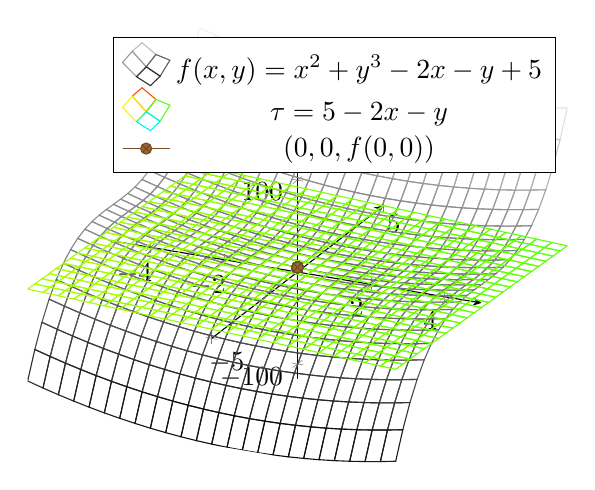
\begin{tikzpicture}
	\begin{axis} [axis lines=middle]
	\addplot3[mesh,colormap/blackwhite]{x^2+y^3-2*x-y+5};\addlegendentry{$f(x,y)=x^2+y^3-2x-y+5$}
	\addplot3[mesh,colormap/bluered]{5-2*x-y};\addlegendentry{$\tau=5-2x-y$}
	\addplot3 ({0},{0},{5});\addlegendentry{$(0,0,f(0,0))$}
	\end{axis}
	\end{tikzpicture}
	\end{center}
	\end{figura}
	\end{ejem}
	
	\begin{observacion} Como consecuencia del ejercicio anterior:\\
	$f(x)=f(a)+df(a)(x-a)+\varphi(x)$ donde $\varphi$ cumple $\limite{\dfrac{f(x)}{\norm{x-a}}}{x\to a}=0$
	\end{observacion}
	
	\begin{ejem} Aproximar $(0,99\cdot \e^{0,02})^{8}$\\
	Consideramos la función $f(x,y)=(x\e^y)^8=x^8\e^{8y}$. Calculemos $f(0'99,0'02)$\\
	$(0,99\cdot \e^{0,02})^{8}=f(0'99,0'02)\approx f(1,0)+df(1,0)(0'99-1,0'02-0)=\\=1+\dotproduct{\gradiente f(1,0)}{(-0'01,0'02)}=1+\dotproduct{(8,8)}{(-0'01,0'02)}=1+8(-0'01+0'02)=1,08$
	\end{ejem}
	
	\begin{proposicion} Condición suficiente de diferenciabilidad.\\
	Sea $U\in\R^n$ abierto, sea $\function{f}{U}{\R}$ y sea $a\in U$. Si $\exists r>0\talque$ en $B(a,r)$ existen las derivadas parciales de $f$ y son continuas en $a$, entonces $f$ es diferenciable en $a$.
	\begin{proof}\ \\
	Queremos probar que $\limite{\dfrac{f(x)-f(a)-\stackbin[i=1]{n}\sum \dfrac{\partial f}{\partial x_i}(a)(x_i-a_i)}{\norm{x-a}}}{x\to a}=0$\\
	Sea $x\in B(a,r)\setminus\{a\}$, entonces, $f(x_1,x_2,...,x_n)-f(a_1,a_2,...,a_n)=\\=
	f(x_1,x_2,...,x_n)-f(a_1,x_2,...,x_n)+f(a_1,x_2,...,x_n)-f(a_1,a_2,x_3,...,x_n)+f(a_1,a_2,x_3,...,x_n)+\\+...-f(a_1,a_2,...,a_{n-1},x_n)+f(a_1,a_2,...,a_{n-1},x_n)-f(a_1,a_2,...,a_n)$\\
	Para cada $i\in\{1,2,...,n\}$ podemos aplicar el teorema del valor medio a la función $\varphi_i(t)=\\=f(a_1,a_2,...,t_i,x_{i+1},...,x_n)$ y obtenemos que $\exists t_i$ entre $x_i$ y $a_i$ tal que $\varphi_i'(t_i)=\dfrac{\varphi(x_i)-\varphi(a_i)}{x_i-a_i}\implies\\ \implies \varphi(x_i)-\varphi(a_i)=\varphi_i'(t_i)(x_i-a_i)=\dfrac{\partial f}{\partial x_i}(a_1,a_2,...,t_i,x_{i+1},...,x_n)(x_i-a_i)$\\
	Por tanto, sea $U_i=(a_1,a_2,...,t_i,x_{i+1},...,x_n)$ tenemos que $\norm{U_i-a}\leq\norm{x-a}$\\
	$f(x)-f(a)=\stackbin[i=1]{n}\sum(\varphi_i(x_i)-\varphi_i(a_i))\stackbin{\mathrm{TVM}}=\stackbin[i=1]{n}\sum\dfrac{\partial f}{\partial x_i} (U_i)(x_i-a_i)$, veamos que tiende a 0.\\
	Por tanto: $0\leq \dfrac{1}{\norm{x-a}}\left|f(x)-f(a)-\stackbin[i=1]{n}\sum\dfrac{\partial f}{\partial x_i}(a)(x_i-a_i)\right|=\\=\dfrac{1}{\norm{x-a}}\left|\stackbin[i=1]{n}\sum\dfrac{\partial f}{\partial x_i} (U_i)(x_i-a_i)-\stackbin[i=1]{n}\sum\dfrac{\partial f}{\partial x_i}(a)(x_i-a_i)\right|\leq\\ \leq \dfrac{1}{\norm{x-a}}\stackbin[i=1]{n}\sum\left|\dfrac{\partial f}{\partial x_i}(U_i)-\dfrac{\partial f}{\partial x_i}(a)\right||x_i-a_i|\leq\dfrac{1}{\norm{x-a}}\cdot\norm{x-a}\stackbin[i=1]{n}\sum\left|\dfrac{\partial f}{\partial x_i}(U_i)-\dfrac{\partial f}{\partial x_i}(a)\right|=\\=
	\stackbin[i=1]{n}\sum\left|\dfrac{\partial f}{\partial x_i}(U_i)-\dfrac{\partial f}{\partial x_i}(a)\right|$\\
	Así, dado $\varepsilon>0$, $\dfrac{\partial f}{\partial x_i}$ es continua en $a$ $\forall i\in\{1,2,...,n\}$, entonces $\exists \delta_1,\delta_2,...,\delta_n>0$ tal que:\\
	$\left|\dfrac{\partial f}{\partial x_i}(x)-\dfrac{f}{x_i}(a)\right|<\dfrac{\varepsilon}{n}\ \forall x\in B(a,\delta_i)$. Tomemos $\delta = \min\{\delta_1,...,\delta_n\}>0$.\\
	Ahora, si $x\in B(a,\delta)\setminus\{a\}$ tenemos que:\\
	$0\leq\dfrac{1}{\norm{x-a}}\left|f(x)-f(a)-\stackbin[i=1]{n}\sum\dfrac{\partial f}{\partial x_i}(a)(x_i-a_i)\right|\leq 
	\stackbin[i=1]{n}\sum\left|\dfrac{\partial f}{\partial x_i}(U_i)-\dfrac{\partial f}{\partial x_i}(a)\right|\leq\stackbin[i=1]{n}\sum\dfrac{\varepsilon}{n}=\varepsilon$
	\end{proof}
	\end{proposicion}
	
	\begin{observacion}Como consecuencia de la proposición anterior, si $\function{f}{U}{\R}$ tiene derivadas parciales y son continuas en $U\subset\R^n$ abierto, entonces $f$ es diferenciable en $u\ \forall u\in U$.
	\end{observacion}
	
	\begin{ejem} Estudia la diferenciabilidad de:\\
	$f(x,y)=\doubleleft{\dfrac{xy^2}{x^2+y^4}\mathrm{\ si\ }(x,y)\neq(0,0)}{\ \ \ \ 0\mathrm{\ \ \ \ \ \ si\ }(x,y)=(0,0)}$\\
	Es claro que $g(x)=\dfrac{xy^2}{x^2+y^4}$ tiene derivadas parciales y son continuas en todo su dominio, $D_g=\R^2\setminus\{(0,0)\}$ y $f\equiv g$ en $\R^2\setminus\{(0,0)\}$. Entonces $f$ tiene derivadas parciales y son continuas en $\R^2\setminus\{(0,0)\}$\\
	Por la proposición anterior, tenemos que $f$ es diferenciable en $\R^2\setminus\{(0,0)\}$. Veamos que ocurre en $(0,0)$. Podemos comprobar que $f$ tiene todas las derivadas direccionales en $(0,0)$, pero $f$ no es diferenciable en $(0,0)$ entre otras cosas porque no es continua en dicho punto.\\ De hecho $\nexists \limite{f(x,y)}{(x,y)\to(0,0)}$. En efecto:\\
	$\limite{f(x,0)}{x\to 0}=0$\\
	$\limite{f(x^2,x)}{x\to 0}=\limite{\dfrac{x^2x^2}{x^4+x^4}}{x\to 0}=\limite{\dfrac{x^4}{2x^4}}{x\to 0}=\dfrac{1}{2}\neq 0$
	\begin{figura}\ \\
	\begin{center}
	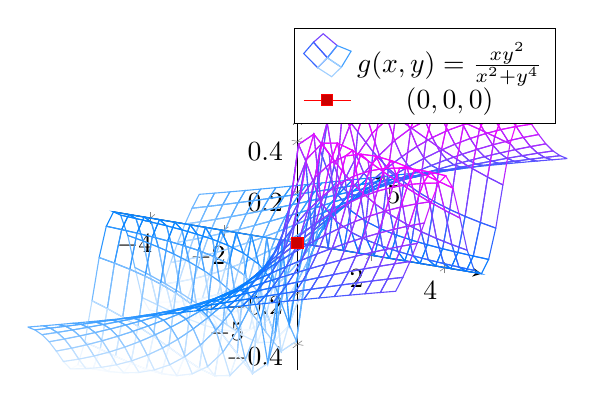
\begin{tikzpicture}
	\begin{axis} [axis lines=middle]
	\addplot3[mesh,colormap/cool, domain=-5:5]{(x*y^2)/(x^2+y^4)};\addlegendentry{$g(x,y)=\frac{xy^2}{x^2+y^4}$}
	\addplot3 ({0},{0},{0}); \addlegendentry{$(0,0,0)$}
	\end{axis}
	\end{tikzpicture}
	\end{center}
	\end{figura}
	\end{ejem}
	
	\begin{observacion}\ \\
	Sea $\doubleright{g\mathrm{\ diferenciable\ en \ }B}{f\equiv g\mathrm{\ en \ }B}\implies f$ es diferenciable en $\mathring{B}$ y $df(a)=dg(a)\ \forall a\in\mathring{B}$
	\end{observacion}
	
	\begin{observacion} Si $f$ es diferenciable en $a$, entonces $f$ es continua en $a$ y tiene todas las derivadas parciales de $f$ en $a$. Además $D_uf(a)=\dotproduct{\gradiente f(a)}{u}\ \forall u\in\R^n$ con $\norm{u}=1$\\
	Como $\dotproduct{\gradiente f(a)}{u}=\norm{\gradiente f(a)} \  \norm{u}\cos(\gradiente f(a),u)=\norm{\gradiente f(a)}\cos(\gradiente f(a),u)$.\\
	Por tanto la derivada direccional maximal de $f$ en $a$ se alcanza en la dirección del vector gradiente $\gradiente f(a)=\left(\dfrac{\partial f}{\partial x_1}(a),\dfrac{\partial f}{\partial x_2}(a),...,\dfrac{\partial f}{\partial x_n}(a)\right)$ y su valor es $\norm{\gradiente f(a)}$.
	\end{observacion}
	
	\section{Diferenciabilidad en funciones de $\R^n$ en $\R^m$}	
	
	\begin{nota} Antes de continuar conviene leer el Apéndice \textsc{A. Repaso de aplicaciones lineales}.\end{nota}
	
	\begin{defi} Sea $U\in \R^n$ abierto, $\xfunction{f}{U}{\R^m}{x\rightarrow(f_1(x),f_2(x),...,f_m(x))}$ y sea $a\in U$. Diremos que $f$ es \textbf{diferenciable en $a$} si $\exists \function{L}{\R^n}{\R^m}$ lineal tal que $\limite{\dfrac{f(a+h)-f(a)-L(h)}{\norm{h}}}{\htiende}=\overline{0}\in\R^m$ o equivalentemente, $\limite{\dfrac{f(x)-f(a)-L(x-a)}{\norm{x-a}}}{x\rightarrow a}=\overline{0}\iff \limite{\dfrac{\norm{f(x)-f(a)-L(x-a)}_{\R^m}}{\norm{x-a}_{\R^n}}}{x\rightarrow a}=\\=0$.
	\begin{observacion} $\limite{\dfrac{f(a+h)-f(a)-L(h)}{\norm{h}}}{\htiende}=\overline{0}\in\R^m\iff \limite{\dfrac{f_i(a+h)-f_i(a)-L_i(h)}{\norm{h}}}{\htiende}=\\=0\in\R$, para $1\leq i\leq m\iff L_i=df_i(a)$ para $1\leq i\leq m$.
	\end{observacion}
	Veamos ahora que si existe dicha $L$, ha de ser $L=(L_,L_2,...,L_m)=(df_1(a),df_2(a),...,df_m(a))$.\\
	Por tanto si existe $L$, es única, la llamamos diferencial de $f$ en $a$ y la denotamos por $df(a)$.
	\begin{observacion}
	$f=(f_1,f_2,f_3,..,f_m)$ es diferenciable en $a\iff f_1,f_2,..,f_m$ son diferenciables en $a$. Además $df(a)=(df_1(a),df_2(a),...,df_m(a))$\\
	Así tenemos que $f$ diferenciable en $a\implies f$ continua en $a$ ya que, $f$ diferenciable en $a\implies f_1,f_2,...,f_m$ diferenciables en $a\implies f_1,f_2,...,f_m$ continuas en $a\implies f$ es continua en $a$.\\
	\end{observacion}
	\end{defi}
	
	\begin{defi} A la matriz asociada a $df(a)$ la denominamos \textbf{matriz jacobiana de $f$ en $a$} y la denotamos por $J_f(a)$.\\
	$J_f(a)=\begin{pmatrix}
	\dfrac{\partial f_1}{\partial x_1}(a) & \dfrac{\partial f_1}{\partial x_2}(a) & \ldots & \dfrac{\partial f_1}{\partial x_n}(a)\\ \dfrac{\partial f_2}{\partial x_1}(a)& \ddots & &\vdots\\ \vdots & & \ddots & \vdots\\ \dfrac{\partial f_m}{\partial x_1}(a)& \ldots & \ldots & \dfrac{\partial f_m}{\partial x_n}(a)
	\end{pmatrix}=\begin{pmatrix}
	D_1f_1(a) & D_2f_1(a) & \ldots & D_nf_1(a)\\ D_1f_2(a)& \ddots & &\vdots\\ \vdots & & \ddots & \vdots\\ D_1f_m(a)& \ldots & \ldots & D_mf_n(a)
	\end{pmatrix}$
	\end{defi}
	
	\begin{ejem} $\xfunction{f}{\R^3}{\R^2}{(x,y,z)\rightarrow(x^2y,3zy^3)}$\\
	$f$ es diferenciable en todo $\R^3$ pues $f_1(x,y,z)=x^2y$ y $f_2(x,y,z)=3zy^3$ tienen derivadas parciales y son continuas en $\R^3$ luego son diferenciables en $\R^3$\\
	$J_f(x,y,z)=\begin{pmatrix} 2xy&x^2&0\\0&9zy^2&3y^3	
	\end{pmatrix}$ en particular $J_f(1,0,2)=\begin{pmatrix}0&1&0\\0&0&0\end{pmatrix}$\\
	$\function{df(1,0,2)}{\R^3}{\R^2}$ donde $(h_1,h_2,h_3)\rightarrow \begin{pmatrix}
	J_f(1,0,2)\begin{pmatrix}h_1\\h_2\\h_3	\end{pmatrix}\end{pmatrix}^t=\begin{pmatrix}
	\begin{pmatrix}0&1&0\\0&0&0	\end{pmatrix} &\begin{pmatrix}h_1\\h_2\\h_3\\	\end{pmatrix}
	\end{pmatrix}^t=\\=\begin{pmatrix}h_2\\0	\end{pmatrix}^t=\begin{pmatrix}h_2 & 0	\end{pmatrix}. $
	\end{ejem}
	
	\begin{ejem} $\xfunction{f}{\R}{\R^3}{t\to (\cos t,\sen t, t)}$\\
	$f_1,f_2,f_3$ son continuas en $\R$, luego $f$ es diferenciable en $\R$ y tenemos:\\
	$J_f(t)=\begin{pmatrix}f_1'(t)\\f_2'(t)\\f_3'(t)\end{pmatrix}= \begin{pmatrix}-\sen(t)\\\cos(t)\\1\end{pmatrix}$
	\end{ejem}
	
	\section{Propiedades de la diferenciabilidad de funciones de $\R^n$ en $\R^m$}	
	
	\begin{proposicion} Sea $U\subset \R^n$ abierto, sean $\function{f\mathrm{\ y\ }g}{U}{\R^m}$ y sea $a\in U$. Si $f$ y $g$ son diferenciables en $a$ entonces $(f+g)$, $(f-g)$ y $\alpha f$ (con $\alpha \in \R$) son diferenciables en $a$ y además:\begin{itemize}
	\item $d(f+g)(a)=df(a)+dg(a)$
	\item $d(f-g)(a)=df(a)-dg(a)$
	\item $d(\alpha f)(a)=\alpha df(a)$
	\end{itemize}
	\begin{proof}\ \\
	A partir de la definición de diferenciabilidad y de la proposición de los límites.	
	\end{proof}
	\end{proposicion}
	
	\begin{teor}\textbf{Regla de la cadena}.\\
		Sea $U\subset \R^n$ abierto, sea $V\subset\R^m$ abierto, sea $\function{f}{U}{\R^m}$, sea $\function{g}{V}{\R^k}$ tal que $f(U)\subset V$ y sea $a\in U$. Si $f$ es diferenciable en $a$ y $g$ es diferenciable en $f(a)$, entonces $g\circ f$ es diferenciable en $a$ y $d(g\circ f)(a)=dg(f(a))\circ df(a)$ y por tanto $J_{g\circ f}(a)=J_g(f(a))\cdot J_f(a)$.
		\begin{ejem} Sean $f(x,y,z)=(x^2y,y+z)$ y $g(u,v)=u\cdot v$ $(\R^3\overset{f}\to\R^2\overset{g}\to \R)$ \\
			$J_{g\circ f}(x,y,z)=J_g(f(x,y,z))\cdot J_f(x,y,z)$
		\end{ejem}
		\begin{proof}\ \\
		Por hipótesis, sea $L=df(a)$ y $S=dg(f(a))$, tenemos:\\
		\begin{enumerate}[a)]
			\item $\dfrac{f(x)-f(a)-L(x-a)}{\norm{x-a}}\overset{x\to a}\longrightarrow 0\ (\in\R^m)$
			\item $\dfrac{g(y)-g(f(a))-S(y-f(a))}{\norm{y-f(a)}}\overset{y\to f(a)}\longrightarrow 0\ (\in\R^k)$
		\end{enumerate}
		Queremos probar:
		\[\dfrac{g(f(x))-g(f(a))-S\circ L(x-a)}{\norm{x-a}}\overset{x\to a}\longrightarrow 0\ (\in\R^k)\]
		Entonces:\\
		Por a), para $\varepsilon_0=1\ \exists r>0 \talque \dfrac{\norm{f(x)-f(a)-L(x-a)}}{\norm{x-a}} < 1\ \forall x\in B(a,r)\setminus\{a\}\implies$\\
		$\implies\norm{f(x)-f(a)-L(x-a)}\leq \norm{x-a}\ \forall x\in B(a,r)\implies \norm{f(x)-f(a)}\leq\\\leq\norm{f(x)-f(a)-L(x-a)}+\norm{L(x-a)}\leq\norm{x-a}+\norm{L}\norm{x-a}=(1+\norm{L})\norm{x-a}\ \forall x\in B(a,r)$\\
		Así tenemos $f$ diferenciable en $a\implies\exists r>0\ \exists M>0 \talque \norm{f(x)-f(a)}\leq M\norm{x-a}\ \forall x\in B(a,r)$\\
		Dado $\varepsilon >0$, buscamos $\delta >0 \talque \dfrac{\norm{g(f(x))-g(f(a))-S\circ L(x-a)}}{\norm{x-a}}<\varepsilon\ \forall x\in B(a,\delta)\setminus\{a\}$\\
		Para $\varepsilon' = \dfrac{\varepsilon}{2(\norm{S}+1)}>0$, por a), tenemos que $\exists\delta_1>0$ tal que:\\
		$\boxed{\dfrac{\norm{f(x)-f(a)-L(x-a)}}{\norm{x-a}}<\varepsilon'\ \forall x \in B(a,\delta_1)\setminus\{a\}}^{\textbf{(*)}}$\\
		Para $\varepsilon'' = \dfrac{\varepsilon}{2M}>0\ \exists\delta_2>0 \talque \dfrac{\norm{g(y)-g(f(a))-S(y-f(a))}}{\norm{y-f(a)}}<\varepsilon''\ \forall y \in B(f(a),\delta_2)\setminus\{f(a)\}\\
		\implies\boxed{\norm{g(y)-g(f(a))-S(y-f(a))}<\varepsilon''\norm{y-f(a)}\ \forall y\in B(f(a),\delta_2)}^{\textbf{(**)}}$\\
		Sea $\delta=\min\{r,\delta_1,\delta_2\}>0$. Ahora si $x\in B(a,\delta)\setminus\{a\}$; es decir, $0<\norm{x-a}<\delta$ tenemos:\\
		$\dfrac{\norm{g(f(x))-g(f(a))-S\circ L(x-a)}}{\norm{x-a}}\stackbin[+\mathrm{\ des.\ triangular}]{\pm S(f(x)-f(a))}\leq\dfrac{\norm{g(f(x))-g(f(a))-S(f(x)-f(a))}}{\norm{x-a}} +\\+ \dfrac{\norm{S(f(x)-f((a))-S\circ L(x-a)}}{\norm{x-a}}$ y ahora por (**) y como $\norm{x-a}<\delta\leq r\implies\\ \implies \norm{f(x)-f(a)}<M\norm{x-a}\leq M\delta\leq M\delta_2$ tenemos que:\\\\
		$\dfrac{\norm{g(f(x))-g(f(a))-S(f(x)-f(a))}}{\norm{x-a}} + \dfrac{\norm{S(f(x)-f(a))-S\circ L(x-a)}}{\norm{x-a}}\leq \\\\
		\leq \dfrac{\varepsilon''\norm{f(x)-f(a)}}{\norm{x-a}}+\norm{S\left(\dfrac{f(x)-f(a)-L(x-a)}{\norm{x-a}}\right)}\stackbin[\implies\norm{f(x)-f(a)}\leq M\norm{x-a}]{x\in B(a,r)\implies}\leq\\ \leq \dfrac{\varepsilon'' M\norm{x-a}}{\norm{x-a}}+\norm{S}\norm{\dfrac{f(x)-f(a)-L(x-a)}{\norm{x-a}}}\stackbin[\norm{x-a}<\delta\leq\delta_1]{\mathrm{Por\ } (*)}< \varepsilon''M+\norm{S}\varepsilon'\leq\dfrac{\varepsilon}{2}+\dfrac{\varepsilon}{2}=\varepsilon$
		\end{proof}
	\end{teor}
	
	\begin{observacion}Como hemos visto antes $J_{g\circ f}(a)=J_g(f(a))\cdot J_f(a)$\\ Escribamos esto matricialmente:\\
	\[\begin{pmatrix} \dfrac{\partial (g\circ f)_1}{\partial x_1}(a) &\hdots&\dfrac{\partial (g\circ f)_1}{\partial x_n}(a)\\ \vdots & \ddots &\vdots\\ \dfrac{\partial (g\circ f)_k}{\partial x_1}(a) &\hdots & \dfrac{\partial (g\circ f)_k}{\partial x_n}(a)	\end{pmatrix}=\]\[=\begin{pmatrix}\dfrac{\partial g_1}{\partial x_1}(f(a))&\hdots & \dfrac{\partial g_1}{\partial x_m}(f(a))\\ \vdots & \ddots &\vdots\\\dfrac{\partial g_k}{\partial x_1}(f(a))&\hdots & \dfrac{\partial g_k}{\partial x_m}(f(a))	\end{pmatrix}\begin{pmatrix}\dfrac{\partial f_1}{\partial x_1}(a)&\hdots & \dfrac{\partial f_1}{\partial x_n}(f(a))\\ \vdots & \ddots &\vdots\\\dfrac{\partial f_m}{\partial x_1}(f(a))&\hdots & \dfrac{\partial f_m}{\partial x_n}(f(a))	\end{pmatrix}\]
	También podemos expresar $(g\circ f)(a)$ como:\\
	\[\dfrac{\partial(g\circ f)_i}{\partial x_j}(a)=\stackbin[l=1]{m}\sum \dfrac{\partial g_i(f(a))}{\partial x_l}\cdot\dfrac{\partial f_i}{\partial x_j}(a)\ \forall 1\leq i\leq k,\ \forall 1\leq j\leq n\]
	\end{observacion}
	
	\begin{proposicion} Sea $U\subset \R^n$ abierto, sean $\function{f\mathrm{\ y\ }g}{U}{\R}$ y sea $a\in U$
	\begin{enumerate}[a)]
	\item Si $f$ y $g$ son diferenciables en $a$ entonces $f\cdot g$ es diferenciable en $a$ y $d(f\cdot g)(a)=f(a)\cdot dg(a)+g(a)\cdot df(a)$.
	\item Si $f$ y $g$ son diferenciables en $a$ y $g(a)\neq 0$ entonces $\dfrac{f}{g}$ es diferenciable en $a$ y $d\left(\dfrac{f}{g}\right)(a)=\dfrac{1}{(g(a))^2}\cdot (g(a)\cdot df(a)-f(a)\cdot dg(a))$.
	\end{enumerate}
	\begin{proof}\ \\
	Demostraremos solo el apartado b).\\
	$g$ diferenciable en $a\implies g$ continua en $a$\\
	$\doubleright{g\mathrm{\ continua\ en\ }a}{g(a)\neq 0}\implies\exists r>0\talque g(x)\neq 0\ \forall x\in B(a,r)$\\
	Luego $\dfrac{f}{g}$ está bien definida en $B(a,r)$. Sean:\\
	$\stackbin[x\longrightarrow(f(x),g(x))]{}{H\colon B(a,r)\rightarrow\R^2\setminus\{(x,0)\talque x\in \R\}}\ \ $ y \\ $\stackbin[(f(x),g(x))\longrightarrow\frac{f(x)}{g(x)}]{}{\Phi\colon\R^2\setminus\{(x,0)\talque x\in \R\}\rightarrow \R}$\\
	Entonces $\dfrac{f}{g}=\Phi\circ H$. $H$ es diferenciable en $a$ (pues sus componentes $f$ y $g$ son diferenciables en $a$). $\Phi$ es diferenciable en todo su dominio.\\
	Por la regla de la cadena $\dfrac{f}{g}=\Phi\circ H$ es diferenciable en $a$ y $d(\dfrac{f}{g})(a)=d\Phi(H(a))\circ dH(a)=\\=d\Phi(f(a),g(a))\circ dH(a)$. Ahora:\\
	$J_{\frac{f}{g}}(a)=J_\Phi(f(a),g(a))\cdot J_H(a)=\begin{pmatrix} \dfrac{1}{g(a)}&-\dfrac{f(a)}{(g(a))^2}\end{pmatrix}\begin{pmatrix}D_1f(a)&D_2f(a)&\hdots&D_nf(a)\\D_1g(a)&D_2g(a)&\hdots&D_ng(a)\end{pmatrix}$\\
	Luego $d(\dfrac{f}{g})(a)=\dfrac{1}{g(a)}\cdot df(a)-\dfrac{f(a)}{(g(a))^2}\cdot dg(a)=\dfrac{1}{(g(a))^2}\cdot(g(a)\cdot df(a)-f(a)\cdot dg(a))$
	\end{proof}
	\end{proposicion}
	
	\section{Derivabilidad en funciones de $\R$ en $\R^n$}
	
	\begin{observacion} Sea $\function{\varphi}{I}{\R^n}$ con $I\subset \R$ intervalo, y sea $\varphi(t)=(\varphi_1(t),\varphi_2(t),...,\varphi_n(t))$\\
	Si $\varphi_1,...,\varphi_n$ son derivables en $t_0\in\mathring{I}$, entonces $\varphi$ es diferenciable en $t_0$ y $J_\varphi(t_0)=\begin{pmatrix}\varphi_1 '(t_0)\\\vdots \\\varphi_n '(t_0)\end{pmatrix}$ Observemos que tiene sentido preguntarse si ¿$\exists \limite{\dfrac{\varphi(t_0+h)-\varphi(t_0)}{h}}{\htiende}$?
	\end{observacion}
	
	\begin{defi} Se dice que $\varphi\colon\R\to\R^n$ es derivable en $t_0$ si $\exists \limite{\dfrac{\varphi(t_0+h)-\varphi(t_0)}{h}}{\htiende}$. Si existe será un vector de $\R^n$ y lo denotaremos por $\varphi'(t_0) = \limite{\dfrac{\varphi(t_0+h)-\varphi(t_0)}{h}}{\htiende} =\\= \left( \limite{\dfrac{\varphi_1(t_0+h)-\varphi_1(t_0)}{h}}{\htiende}, \limite{\dfrac{\varphi_2 (t_0+h)-\varphi_2 (t_0)}{h}}{\htiende},\ ...\ ,\limite{\dfrac{\varphi_n(t_0+h)-\varphi_n(t_0)}{h}}{\htiende}\right) =\\= (\varphi_1'(t_0),\varphi_2'(t_0),...,\varphi_n'(t_0))$
	\end{defi}
	
	\begin{observacion} Por tanto tenemos que $\varphi$ es derivable en $t_0 \iff \varphi_i\ $ es derivable en $t_0\\ \forall\ 1\leq i\leq n$
	\end{observacion}
	
	\begin{defi} Si $\varphi$ es continua en $I\subset\R$ decimos que $\Gamma:=\varphi(I)$ es una curva en $\R^n$ parametrizada por $\varphi$. Además, si $\varphi$ es derivable en $t_0\in I$, la recta tangente a $\Gamma$ en $\varphi(t_0)$ es la recta que pasa por dicho punto y tiene como vector director $\varphi'(t_0)$.
	\end{defi}
	
	\begin{observacion} Sea $I\subset\R$ y sea $\function{\varphi}{I}{\R^n}$. Si $\varphi$ es derivable en $t_0$, ya hemos visto que $\varphi'(t_0)=(\varphi'_1(t_0),\varphi'_2(t_0),...,\varphi'_n(t_0))$. Entonces:\\
	$J_\varphi(t_0)=\begin{pmatrix}\varphi'_1(t_0) \\ \varphi'_2(t_0) \\ \vdots \\ \varphi'_n(t_0)\end{pmatrix}$ y por tanto, $\ \xfunction{d\varphi (t_0)}{\R}{\R^n}{h\to h(\varphi'_1(t_0),...,\varphi'_n(t_0))= h\varphi'(t_0)}$
	\end{observacion}
	
	\begin{proposicion} Caso particular de la regla de la cadena para funciones de $\R$ en $\R^n$.\\
	Sea $I\subset\R$, sea $\function{\varphi}{I}{R^n}$ diferenciable en $t_0\in\mathring{I}$, sea $U\subset\R^n$ abierto tal que $\varphi(I)\subset U$ y sea $\function{f}{U}{\R}$ diferenciable en $\varphi(t_0)$.\\
	Sea $g(t):=f(\varphi(t))\ \forall t\in I$ es derivable en $t_0$ y $g'(t_0)=\dotproduct{\gradiente f(\varphi(t_0))}{\varphi'(t_0)}$ ya que\\ $g'(t_0)\equiv J_g(t_0)=J_f(\varphi(t_0))\cdot J_\varphi(t_0)=\begin{pmatrix}\dfrac{\partial f}{\partial x_1}(\varphi(t_0)) & \dfrac{\partial f}{\partial x_2}(\varphi(t_0))& \hdots & \dfrac{\partial f}{\partial x_n}(\varphi(t_0))	\end{pmatrix}\begin{pmatrix}\varphi'_1(t_0) \\ \varphi'_2(t_0) \\ \vdots \\ \varphi'_n(t_0)\end{pmatrix}=\\=\dotproduct{\gradiente f(\varphi(t_0))}{(\varphi'_1(t_0),...,\varphi'_n(t_0))}=\dotproduct{\gradiente f(\varphi(t_0))}{\varphi'(t_0)}$
	\end{proposicion}
	
	\section{Teorema del valor medio. Teorema de los incrementos finitos}
	\begin{teor} \textbf{Teorema del valor medio (de $\R$ en $\R$)}\\
	Si $\function{f}{[a,b]}{\R}$ es continua en $[a,b]$ y derivable en $(a,b)$ entonces $\exists c\in (a,b)$ tal que $f(b)-f(a)=f'(c)(b-a)$.
	\end{teor}
	
	\begin{observacion} ¿Se cumple el siguiente ``teorema del valor medio'' de $\R^n$ en $\R^m$?\\
	Sea $\function{f}{U\subset\R^n}{\R^m}$, si $f$ es diferenciable en $U$ y $a,b\in U$.\\
	¿$\exists c\in U\talque f(b)-f(a)=df(c)(b-a)$? ó ¿$\exists c \in [a,b]\setminus\{a,b\}\talque f(b)-f(a)=df(c)(b-a)$?\\
	En general no.
	\begin{ejem} Sea $\xfunction{\varphi}{[0,1]}{\R^2}{t\to (1-t^2,1-t^3)}$\\
	Tenemos $\varphi(1)-\varphi(0) = (0,0)-(1,1)=(-1,-1)$\\
	Además $\varphi'(t)=(-2t,-3t^2)\implies d\varphi(c)(b-a)=\varphi'(c)(1-0)=(-2c,-3c^2)$ y tenemos que $\nexists c\in (0,1)\talque (-1,-1)=(-2c,-3c^2)$.
	\end{ejem}
	\begin{nota} Si el espacio de llegada es $\R^m$ com $m>1$, el teorema del valor medio, en general, no se cumple. \end{nota}
	\end{observacion}
	
	\begin{observacion} Nos preguntamos ahora:\\
	Sea $\function{f}{U}{\R}$ diferenciable en $U$ (abierto contenido en $\R^n$) y $a,b\in U$.\\
	¿$\exists c\in U\talque f(b)-f(a)=df(c)(b-a)$?\\
	En general no.
	\begin{ejem} Sea $\xfunction{f}{\R^2\setminus\{(x,0)\talque x\leq 0\}}{\R}{(x,y)\to \doubleleft{x^2\mathrm{\ si\ }x<0,\ y<0}{0\mathrm{\ en\ resto\ de\ casos}}}$\\
	$f$ es diferenciable en su dominio.\\
	Tenemos que $\dfrac{\partial f}{\partial y}(x,y)=0\ \forall(x,y)\in \dom f$
	Entonces $f(-1,1)-f(-1,-1)=0-1=-1$\\
	$df(c_1,c_2)((-1,1)-(-1,-1))=\dotproduct{\gradiente f(c_1,c_2)}{(0,2)}=\dotproduct{\left(\dfrac{\partial f}{\partial x}(c),\dfrac{\partial f}{\partial y}(c)\right)}{(0,2)}=\\=0\neq -1\ \forall c\in\dom f$
	\end{ejem}
	\end{observacion}
	
	\begin{teor} \textbf{Teorema del valor medio en funciones de $\R^n$ en $\R$}\\
	Sea $U\subset R^n$ abierto, sea $\function{f}{U}{\R}$ diferenciable en $U$ y sean $a,b\in U$ tales que $[a,b]\subset U$. Entonces $\exists c\in [a,b]\setminus\{a,b\}$ tal que $f(b)-f(a)=df(c)(b-a)$
	\begin{proof}\ \\
	Definamos $\xfunction{g}{[0,1]}{\R}{t\to f((1-t)a+tb)}$\\
	Observamos que $ g(t)=f((1-t)a_1+tb_1,(1-t)a_2+tb_2,\ ...\ ,(1-t)a_n+tb_n)=(f\circ\varphi)(t)$ donde $\xfunction{\varphi}{[0,1]}{\R^n}{t\to (1-t)a+tb}$\\
	Como $\varphi([0,1])=[a,b]\subset U$, $\varphi$ es diferenciable en $[0,1]$ y $f$ es diferenciable en $U\ \ximplies{\mathrm{por\ la \ regla\ de\ la\ cadena}}{}\\ \implies$ tenemos que $g$ es diferenciable en $(0,1)$ y continua en $[0,1]$ pues $\varphi$ y $f$ lo son.\\
	Por el teorema del valor medio (de $\R$ en $\R$) aplicado a $g$, sabemos que existe $t_0\in (0,1)$ tal que $g(1)-g(0)=g'(t_0)(1-0)=g'(t_0)$\\
	Como $g(1)-g(0)=f(b)-f(a)=g'(t_0)=(f\circ\varphi)'(t_0)=\dotproduct{\gradiente f(\varphi(t_0))}{\varphi'(t_0)}$\\
	Llamemos $c=\varphi(t_0)=(1-t_0)a+t_0b\in [a,b]\setminus\{a,b\}$\\
	Tenemos que  $\varphi(t)=(1-t)a+tb\implies \varphi'(t)=b-a\ \forall t\in (0,1)$ y por tanto:\\
	$f(b)-f(a)=\dotproduct{\gradiente f(c)}{\varphi'(t_0)}=\dotproduct{\gradiente f(c)}{b-a}=df(c)(b-a)$
	\end{proof}
	\end{teor}
	
	\begin{teor}\textbf{Teorema de los incrementos finitos}\\
	Sea $U\subset \R^n$ abierto y sea $\function{f}{U}{\R^m}$ diferenciable en $U$. Si $a,b\in U$ tal que $[a,b]\subset U$ entonces $\norm{f(b)-f(a)}\leq\underset{x\in [a,b]}\sup\norm{df(x)}\norm{b-a}$
	\begin{corolario} Antes de demostrar el teorema veamos el siguiente corolario:\\
	Sea $U\subset\R^n$ abierto, $\function{f}{U}{\R^m}$ diferenciable en $U$ y sea $v\in\R^m$. Si $a,b\in U$, con $a\neq b$ tales que $[a,b]\subset U$, entonces $\exists c\in[a,b]\setminus\{a,b\} \talque \dotproduct{v}{f(b)-f(a)}=\dotproduct{v}{df(c)(b-a)}$
	\begin{proof}\ \\
	Definamos $\xfunction{g}{U}{\R}{x\rightarrow\dotproduct{v}{f(x)}}$\\
	Si $v=(v_1,v_2,...,v_m)$, tenemos que $g(x)=v_1f_1(x)+v_2f_2(x)+\ ...\ + v_mf_m(x)\ \forall x\in U$. Como $f$ es diferenciable en $U\implies f_1,f_2,...,f_m$ es diferenciable en $U\implies g$ es diferenciable en $U$ por ser combinación lineal de funciones diferenciables en $U$.\\
	Por el Teorema del valor medio aplicado a $g$ tenemos que $\exists c\in[a,b]\setminus\{a,b\}$ tal que\\
	 $g(b)-g(a)=dg(c)(b-a)$ y por tanto: $g(b)-g(a)=\dotproduct{v}{f(b)}-\dotproduct{v}{f(a)}=\\=\dotproduct{v}{f(a)-f(b)}=dg(c)(b-a)=\stackbin[i=1]{m}\sum v_idf_i(c)(b-a)=\\=\dotproduct{(v_1,v_2,...,v_m)}{(df_1(c),df_2(c),...,df_m(c))(b-a)}=\dotproduct{v}{df(c)(b-a)}$
	\end{proof}
	\end{corolario}
	\begin{proof} Demostremos ahora el Teorema de los incrementos finitos.\\
	Sean $a,b\in U,\ a\neq b$ con $[a,b]\subset U$. Si $\{\norm{df(x)}:x\in [a,b]\}$ no es acotado, entonces la desigualdad del enunciado no dice nada (porque no hay supremo).\\
	Si es acotado, entonces tiene supremos en $\R$\\
	Si $f(a)=f(b)$ trivial.
	si $f(a)\neq f(b)\implies \norm{f(b)-f(a)}>0$. Tomamos $v=\dfrac{f(b)-f(a)}{\norm{f(b)-f(a)}}\\
	(\in R^m)$ y $\norm{v}=1$. Por el corolario anterior $\exists c\in [a,b]\setminus\{a,b\}$ tal que\\
	$\dotproduct{\dfrac{f(b)-f(a)}{\norm{f(b)-f(a)}}}{f(b)-f(a)}=\dotproduct{v}{df(c)(b-a)}$. Luego $\norm{f(b)-f(a)}=\\
	=\dotproduct{v}{df(c)(b-a)}\leq |\dotproduct{v}{df(c)(b-a)}|\overset{\mathrm{desigualdad\ Cauchy-Schwarz}}\leq\norm{v}\norm{df(c)(b-a)}=\\
	=\norm{df(c)(b-a)}\leq\norm{df(c)}\norm{b-a}\leq \underset{x\in [a,b]}\sup\norm{df(x)}\norm{b-a}$	
	\end{proof}
	\end{teor}
	\newpage
	\begin{corolario} Veamos las siguientes consecuencias.
	\begin{enumerate}[1)]
	\item Sea $U\subset\R^n$ abierto y \underline{conexo} y $\function{f}{U}{\R^m}$ diferenciable en $U$. Si $df(x)=0\\
	\forall x\in U\implies f$ es constante en $U$.
	\begin{proof}\ \\
	Por el \textit{Teorema de los incrementos finitos} y la hipótesis tenemos que $f$ es constante en los segmentos contenidos en $U$ y por tanto en los poligonales de $U$. Fijemos $x_0\in U$, por ser $U$ conexo $\implies U$ es conexo por poligonales. Así $\forall x\in U\setminus\{x_0\}\ \exists\Gamma_x$ poligonal en $U$ que une $x$ y $x_0$, luego $f(x)=f(x_0)\implies f$ constante en $U$.
	\end{proof}
	\item Sea $U\subset\R^n$ abierto y \underline{convexo} y sea $\function{f}{U}{\R^m}$ diferenciable en $U$. Si\\
	$\exists M>0\talque \norm{df(x)}\leq M\ \forall x\in U\implies \norm{f(y)-f(x)}\leq M\norm{y-x}\ \forall x,y\in U$.
	\begin{proof}\ \\
	Sean $x,y\in U, x\neq y$. Como $U$ es convexo tenemos $[x,y]\subset U$ y por el \textit{Teorema de los incrementos finitos} tenemos, $\norm{f(y)-f(x)}\leq \underset{z\in [x,y]}\sup\norm{df(z)}\norm{y-x}\leq M\norm{y-x}$
	\end{proof}
	\end{enumerate}
	\end{corolario}
	
	\section{Derivadas parciales de orden superior}
	
	\begin{defi} Derivadas parciales de orden superior.\\
	Sea $U\subset \R^m$ abierto y $\function{f}{U}{\R}$ si $f$ tiene derivadas parciales en $U$ podemos considerar las funciones $\xfunction{D_if}{U}{\R}{x\to D_if(x)}$.\\
	En el caso de que una de estas funciones $D_if$ tenga derivadas parciales en $a\in U$, denominamos a estas \textbf{derivadas parciales segundas} de $f$ en $a$ y las denotamos por:
	\begin{center} $D_j(D_if)(a)\ \ $ ó $\ \ D_{ji}f(a)\ \ $ ó $\ \ \dfrac{\partial^2f}{\partial_{x_j}\partial_{x_i}(a)}$\end{center}
	Además, si $j=i$, solemos escribir $D_{ii}f(a)\ \ $ ó $\ \ \dfrac{\partial^2f}{\partial x^2_i}f(a)$.\\
	Por recurrencia definimos las derivadas parciales terceras, cuartas, ... y $k$-ésimas.
	\end{defi}
	
	\begin{ejem} Sea $f(x,y,z)=3x^2y^3z$, sus derivadas parciales son:
	\begin{center}$D_1f=6xy^3z,\ D_2f=9x^2y^2z,\ D_3f=3x^2y^3$	\end{center}
	Mientras que sus derivadas parciales segundas son:
	\begin{center}$D_{11}f=6y^3z,\ D_{21}f=18xy^2z,\ D_{31}f=6xy^3$	\end{center}
	\begin{center}$D_{12}f=18xy^2z,\ D_{22}f=18x^2yz,\ D_{32}f=9x^2y^2$	\end{center}
	\begin{center}$D_{13}f=6xy^3,\ D_{23}f=9x^2y^2,\ D_{33}f=0$	\end{center}
	\end{ejem}
	
	\begin{defi} Sea $U\subset\R^n$ abierto y sea $\function{f}{U}{\R}$. Decimos que $f$ es de \textit{clase 1} en $U$ y escribimos $f\in C^1(U)$ ó $f$ es $C^1$ en $U$ si posee todas las derivadas parciales y son continuas en $U$.\\ 
	Además, decimos que $f$ es de \textit{clase 2} en $U$ y escribimos $f\in C^2(U)$ ó $f$ es $C^2$ en $U$ si posee todas las derivadas parciales segundas y son continuas en $U$.\\
	Por recursión definimos que $f$ es de \textit{clase $k$} en $U$ y escribimos $f\in C^k(U)$ ó $f$ es $C^k$ en $U$ si posee todas las derivadas parciales $k$-ésimas y son continuas en $U$.
	Si $f\in C^k(U)\ \forall k\in\N$ escribimos $f\in C^\infty(U)$.\\
	Por último, sea $\function{f}{U\subset\R^n}{\R^m}$ con $f=(f_1,f_2,...,f_m)$, decimos que $f\in C^k(U)$ si $f_i\in C^k(U)\ \ \ \forall 1\leq i\leq m$.
	\end{defi}
	
	\begin{observacion} Si $f\in C^1(U)$, entonces $f$ es diferenciable en $U$ y $\function{df}{U}{L(\R^n,\R)}$ es continua.
	\end{observacion}
	
	\begin{teor} Teorema de Schwarz\\
	Sea $U\subset\R^n$ abierto y sea $\function{f}{U}{\R}$, si $f\in C^2(U)$ entonces $D_{ij}f(a) = D_{ji}f(a)\\
	\forall a\in U,\ \ \forall i,j\in\{1,2,...,n\}$.
	\begin{proof}\ \\
	Sea $a\in U$, sean $i,j\in\{1,2,...,n\}$, si $i=j$ trivial.\\
	Si $i\neq j$, como $a\in U$ y $U$ es abierto, $\exists  r_0>0\talque B(a,r_0)\subset U$.\\
	$\boxed{\mathrm{Probemos\ que\ }\forall r\in\left(0,\dfrac{r_o}{2}\right)\ \exists x_r,y_r\in B(a,2r)\talque D_{ij}f(x_r)=D_{ji}f(y_r)}$ \textbf{(*)}\\
	Una vez probado esto tenemos que $\forall n\in \N\ \exists x_n,y_n \in B\left(a,\dfrac{r_o}{n}\right)\talque D_{ij}f(x_n)=D_{ji}f(y_n)$\\
	Así, $x_n\limited a$ e $y_n\limited a$ y como $D_{ij}f\y D_{ji}f$ son continuas en $a$, tenemos:\\
	$D_{ij}f(x_n)\limited D_{ij}f(a)\y D_{ji}f(y_n)\limited D_{ji}f(a)$ y como $D_{ij}f(x_n)=D_{ji}f(y_n)\ \forall n\in N$, tenemos que $D_{ij}f(a)=D_{ji}f(a)$.\\
	Probemos ahora \textbf{(*)}. Definamos las funciones,\\
	$\Phi_1(t)=f(a+r{e_j}+t{e_i})-f(a+t{e_i})\ \forall t\in [0,r]$\\
	$\Phi_2(t)=f(a+r{e_i}+t{e_j})-f(a+t{e_j})\ \forall t\in [0,r]$\\
	Tenemos que $\Phi_1(r)-\Phi_1(0)=\Phi_2(r)-\Phi_2(0)$, ya que:\\
	$\Phi_1(r)-\Phi_1(0)= f(a+re_j+re_i)-f(a+re_i)-f(a+re_j)+f(a)$\\
	$\Phi_2(r)-\Phi_2(0)= f(a+re_i+re_j)-f(a+re_j)-f(a+re_i)+f(a)$\\
	Observamos que el cuadrado de vértices $a$, $a +re_i$, $a+re_j$ y $a +re_i+re_j$ está contenido en $B(a,2r)\subset B(a,r_0)\subset U$.\\
	Por \textit{la regla de la cadena} $\Phi_1\y\Phi_2$ son derivables en $[0,r]$ y por el \textit{teorema del valor medio aplicado} a $\Phi_1$ en $[0,r]$ tenemos que $\exists\alpha\in(0,r)$ tal que:\\
	$\Phi_1(r)-\Phi_1(0)=\Phi_1'(\alpha)(r-0)=r(\dotproduct{\gradiente f(a+re_j+\alpha e_i)\ }{\ e_i}-\dotproduct{\gradiente f(a+\alpha e_i)\ }{\ e_i})=\\
	=r(D_if(a+re_j+\alpha e_i)-D_if(a+\alpha e_i))$.\\
	Aplicando de nuevo el \textit{teorema del valor medio} en $\varphi_1(t)=D_if(a+\alpha e_i+te_j)\ \forall t\in[0,r]$ tenemos que $\exists \beta\in (0,r)\talque \varphi_1(r)-\varphi_1(0)=\varphi_1'(\beta)r=r(D_{ji}f(a+\alpha e_1+\beta e_j))$.\\
	Por tanto $\Phi_1(r)-\Phi_1(0)=r^2(D_{ji}f(a+\alpha e_i+\beta e_j))$.\\
	Razonando análogamente con $\Phi_2$ tenemos que $\exists \oversim{\alpha},\oversim{\beta}\in(0,r)$ tal que:\\
	$\Phi_2(r)-\Phi_2(0)=r^2(D_{ij}f(a+\oversim{\alpha} e_i+\oversim{\beta} e_j))$. Y ahora:\\
	$\Phi_1(r)-\Phi_1(0)=\Phi_2(r)-\Phi_2(0)\y r>0\implies D_{ji}f(a+\alpha e_1+\beta e_j)=D_{ij}f(a+\oversim{\alpha} e_i+\oversim{\beta} e_j)$\\
	Luego llamando $x_r = a+\oversim{\alpha} e_i+\oversim{\beta} e_j$ e $y_r = a+\alpha e_1+\beta e_j\implies x_r,y_r\in B(a,2r)\y D_{ij}f(x_r)=\\
	=D_{ji}f(y_r)$.
	\end{proof}
	\end{teor}
	
	\begin{corolario} Sea $U\subset\R^n$ abierto y sea $\function{f}{U}{\R}$. Si $f\in C^3(U)$, entonces\\
	$D_{ijk}f(a)=D_{\sigma(i)\sigma(j)\sigma(k)}f(a)\ \forall a\in U,\ \forall i,j,k\in\{1,2,...,n\},\ \forall\function{\sigma}{\{i,j,k\}}{\{i,j,k\}}$ biyectiva (o permutación).
	\begin{proof}\ \\
	Sean $i,j,k\in\{1,2,...,n\}$, supongamos que $\sigma(i)=j$, $\sigma(j)=k$, $\sigma(k)=i$ y sea $a\in U$:\\
	$D_{\sigma(i)\sigma(j)\sigma(k)}f(a)=D_{jki}f(a)=D_j(D_{ki}f(a))\overset{\mathrm{T.\ de\ Schwarz}}=D_j(D_{ik}f(a))=D_{jik}f(a)=\\
	=D_{ji}(D_kf(a))\overset{\mathrm{T.\ de\ Schwarz}}=D_{ij}(D_kf(a))=D_{ijk}f(a)$.\\
	Análogamente para el resto de permutaciones.
	\end{proof}
	\end{corolario}
	
	\begin{corolario} Así, por inducción:\\
	Sea $U\subset\R^n$ abierto y sea $\function{f}{U}{\R}$. Si $f\in C^k(U)$, entonces:\\
	$D_{i_1i_2...i_k}f(a)=D_{\sigma(i_1)\sigma(i_2)...\sigma(i_k)}f(a)\ \forall a\in U,\ \forall i_1,i_2,...,i_k\in\{1,2,...,n\},\\
	\forall\function{\sigma}{\{i_1,i_2,...,i_k\}}{\{i_1,i_2,...,i_k\}}$ biyectiva (o permutación).
	\end{corolario}
	
	\section{Teorema de Taylor}

	\begin{nota} No hay \textit{Teorema de Taylor} para funciones que llegan a $\R^m$ con $m>1$.\end{nota}
	\begin{observacion} Recordemos que sea $U\subset \R^n$ abierto y $\function{f}{U}{\R}$ diferenciable en $U$, sea $a\in U\y h\in\R^n\talque [a,a+h]\subset U$ y llamamos:\\
	$\xfunction{\varphi}{[0,1]}{\R^n}{t\to a+th}$, con $\varphi'(t)=(h_1,h_2,...,h_n)\y\varphi''(t)=0\ \forall t\in[0,1]$.\\
	Por la regla de la cadena $\dfrac{d}{dt}(f\circ \varphi)(t)=\dotproduct{\gradiente f(\varphi(t))}{\varphi'(t)}=\dotproduct{\gradiente f(a+th)}{h}$
	\end{observacion}
	
	\begin{teor} Teorema de Taylor (funciones de $\R$ en $\R$).\\
	Sea $\function{g}{I\subset\R}{\R}$ con $g\in C^{k+1}(I)$ y sea $a\in I$, entonces $\forall x\in I\setminus\{0\}\ \exists c$ entre $x\y a\\
	(\in I)$ tal que:\\
	$f(x)=f(a)+\dfrac{f'(a)}{1!}(x-a)+\dfrac{f''(a)}{2!}(x-a)^2+...+\dfrac{f^{(k)}(a)}{k!}(x-a)^k+\dfrac{f^{(k+1)}(c)}{(k+1)!}(x-a)^{k+1}$\\
	O escrito de otro modo, fijado $a\in I,\ \forall h\in\R\talque a+h\in I,\ \exists c$ entre $a\y a+h$ tal que:
	$f(a+h)=\underset{P_{k,a}(h)}{\underbrace{f(a)+\dfrac{f'(a)}{1!}h+\dfrac{f''(a)}{2!}h^2+...+\dfrac{f^{(k)}(a)}{k!}h^k}}+\dfrac{f^{(k+1)}(c)}{(k+1)!}h^{k+1}$
	\end{teor}
	
	\begin{observacion} $\limite{}{h\to 0}\dfrac{f(a+h)-P_{k,a}(h)}{h^k}=0$\end{observacion}
	
	\begin{teor} Teorema de Taylor.\\
	Sea $U\subset\R^n$ abierto, sea $k\in\N$, sea $\function{f}{U}{\R}$ con $f\in C^{k+1}(U)$ y sea $a\in U$. Entonces $\forall h\in\R^n$ tal que $[a,a+h]\subset U,\ \exists c\in [a,a+h]\setminus\{a,a+h\}$ tal que: $f(a+h)=$\[=\underset{\mathrm{Polinomio\ de\ Taylor\ de\ }f\ \mathrm{de\ orden\ }k\ \mathrm{en\ }a\ (P_{k,a})}{\underbrace{f(a)+\stackbin[j=1]{k}\sum\dfrac{1}{j!}\left(\stackbin[i_1,...,i_j=1]{n}\sum h_{i_1}\cdot\cdot\cdot h_{i_j}D_{i_1...i_j}f(a)\right)}}+\underset{\mathrm{Resto\ de\ Taylor\ (R_{k,a})}}{\underbrace{\dfrac{1}{(k+1)!}\stackbin[i_1,...,i_{k+1}=1]{n}\sum h_{i_1}\cdot\cdot\cdot h_{i_{k+1}}D_{i_1...i_{k+1}}f(c)}}\]
	\begin{proof}\ \\
	Sea $\varphi(t)=a+th$, sabemos que $\varphi\in C^\infty(\R)$. Como $U$ es abierto y $\varphi$ es continua, entoces $A:=\varphi^{-1}(U)$ es abierto en $\R$.\\
	$\doubleright{\function{\varphi}{A}{\R^n}\mathrm{\ es\ }C^\infty\ \mathrm{en\ }A}{\function{f}{U}{\R}\mathrm{\ es\ }C^{k+1}\ \mathrm{en\ }U}\ximplies{\mathrm{Regla\ de\ la\ cadena}}{}f\circ\varphi$ es $C^{k+1} $ en $A$.\\
	Llamemos $g=f\circ\varphi; \function{g}{A}{\R}$, $g(1)=f(\varphi(1))=f(a+h)\y g(0)=f(\varphi(0))=f(a)$.\\
	Por el \textit{por el teorema de Taylor en $\R$} aplicado a $g$, $\exists\theta\in(0,1)$ tal que:\\
	$g(1)=g(0)+\dfrac{g'(0)}{1!}(1-0)+\dfrac{g''(0)}{2!}(1-0)^2+...+\dfrac{g^{(k)}(0)}{k!}(1-0)^k+\dfrac{g^{k+1}(\theta)}{(k+1)!}(1-0)^{k+1}=\\
	=g(0)+\dfrac{g'(0)}{1!}+\dfrac{g''(0)}{2!}+...+\dfrac{g^{(k)}(0)}{k!}+\dfrac{g^{k+1}(\theta)}{(k+1)!}=$ \textbf{(*)}. Veamos ahora:\\
	$g'(t)=\dfrac{d}{dt}(f\circ\varphi)(t)=\dotproduct{\gradiente f(\varphi(t))}{\varphi'(t)}=\dotproduct{\gradiente f(a+th)}{h}=\stackbin[i=1]{n}\sum h_iD_if(a+th)$.\\
	$g''(t)=\dfrac{d}{dt}\left(\stackbin[i=1]{n}\sum h_iD_if(a+th)\right)=\stackbin[i=1]{n}\sum h_i\dfrac{d}{dt}(D_if(a+th))=\stackbin[i=1]{n}\sum h_i\left(\stackbin[j=1]{n}\sum h_jD_{ji}f(a+th)\right)=\\
	=\stackbin[i=1]{n}\sum \stackbin[j=1]{n}\sum h_i h_jD_{ji}f(a+th)\overset{\mathrm{T.\ Schwarz}}=\stackbin[i=1]{n}\sum \stackbin[j=1]{n}\sum h_i h_jD_{ij}f(a+th)$. Y así por inducción tenemos:\\
	$g^{(k)}=\stackbin[i_1,i_2,...i_k=1]{n}\sum h_{i_1} h_{i_2}\cdot\cdot\cdot h_{i_k}D_{i_1i_2...i_k}f(a+th)$. Y ahora, para acabar:\\
	$f(a+h)=$\textbf{(*)}$=$\\
	$=f(a)+\dfrac{\stackbin[i=1]{n}\sum h_iD_if(a)}{1!}+\dfrac{\stackbin[i,j=1]{n}\sum h_i h_jD_{ij}f(a)}{2!}+...+\dfrac{\stackbin[i_1,i_2,...i_k=1]{n}\sum h_{i_1} h_{i_2}\cdot\cdot\cdot h_{i_k}D_{i_1i_2...i_k}f(a)}{k!}+\\
	+\dfrac{\stackbin[i_1,i_2,...i_k=1]{n}\sum h_{i_1} h_{i_2}\cdot\cdot\cdot h_{i_{k+1}}D_{i_1i_2...i_{k+1}}f(a+\theta h)}{(k+1)!}$
	\end{proof}
	\end{teor}
	
	\begin{nota} Sabiendo que $\alpha_1,\alpha_2,...,\alpha_n\in\R$ entonces $(\alpha_1+\alpha_2+...+\alpha_n)^k=\stackbin[i_1,...,i_k=1]{n}\sum\alpha_{i_1}\hdots\alpha_{i_k}$, se usa la siguiente notación:\\
	$\stackbin[i_1,i_2,...i_k=1]{n}\sum h_{i_1} h_{i_2}\hdots h_{i_k}D_{i_1i_2...i_k}f(a)=(h_1D_1+h_2D_2+...+h_nD_n)^kf(a)$ y con esta notación tenemos que $P_{k,a}=f(a)+\stackbin[j=1]{k}\sum\dfrac{(h_1D_1+h_2D_2+...+h_nD_n)^jf(a)}{j!}$
	\end{nota}
	
	\begin{ejem} Sea $f(x,y)=\e^xy$, halla $P_{3,(0,1)}$.\\
	$P_{3,(0,1)}=f(0,1)+\dfrac{h_1D_1f(0,1)+h_2D_2f(0,1)}{1!}+\dfrac{h_1^2D_{11}f(0,1)+2h_1h_2D_{12}f(0,1)+h_2^2D_{22}f(0,1)}{2!}+\\
	+\dfrac{h_1^3D_{111}f(0,1)+3h_1^2h_2D_{112}f(0,1)+3h_1h_2^2D_{122}f(0,1)+h_2^3D_{222}f(0,1)}{3!}$\\
	$\doubleleft{D_1f=\e^xy\doubleleft{D_{11}f=e^xy\doubleleft{D_{111}f=e^xy}{D_{211}f=e^x}}{D_{21}f=e^x\{D_{221}f=0}}{D_2f=e^x\{D_{22}f=0}$\\\\
	Luego $P_{3,(0,1)}(h_1,h_2)=\overset{P_{2,(0,1)}}{\overbrace{\underset{P_{1,(0,1)}}{\underbrace{1+(h_1+h_2)}}+\dfrac{h_1^2+2h_1h_2}{2}}}+\dfrac{h_1^3+3h_1^2h_2}{6}$
	\end{ejem}
	
	\begin{observacion} El \textit{teorema de Taylor} nos dice que si $f\in C^{k+1}(U)$ entonces $\forall h\in\R^n$ tal que $[a,a+h]\subset U,\ \exists c_h\in[a,a+h]\talque f(a+h)=P_{k,a}(h)+\boxed{\dfrac{(h_1D_1+...+h_nD_n)^{k+1}f(c_h)}{(k+1)!}}$. A esta último polinomio se le llama \textit{resto de Taylor} de orden $k$ de $f$ en $a$ y se denota por $R_{k,a}(h)$, es decir, $R_{k,a}(h)=f(a+h)-P_{k,a}(h)$.\\
	Si cambiamos $x=a+h$ nos queda:\\
	$f(x)=P_{k,a}(x-a)+\dfrac{((x_1-a_1)D_1+...+(x_n-a_n)D_n)^{k+1}f(c_x)}{(k+1)!}$.\\
	Observemos que si $f\in C^{k+1}(U)$ y tomamos $r>0\talque\overline{B}(a,r)\subset U$, entonces $\forall	h\in\R^n$ con $\norm{h}<r$ tenemos que $\exists c_h\in ()$ tal que:\\
	$|f(a+h)-P_{k,a}(h)|=|R_{k,a}(h)|=\dfrac{\left|\stackbin[i_1...i_{k+1}=1]{n}\sum h_{i_1}\hdots h_{i_{k+1}}D_{i_1\hdots i_{k+1}}f(c_h)\right|}{(k+1)!}\leq\dfrac{M(|h_1|+...+|h_n|)}{(k+1)!}\leq\\
	\leq\dfrac{M}{(k+1)!}(\sqrt{n}\norm{h})^{k+1}$, donde $M=$ máx. de derivadas de orden $k+1$ de $f$ en $\overline{B}(a,r)$. Así, tenemos $\dfrac{|f(a+h)-P_{k,a}(h)|}{\norm{h}^k}\leq\dfrac{Mn^{\frac{k+1}{2}}}{(k+1)!}\norm{h}\ \forall h\in\R^n$ con $\norm{h}<r$. Luego\\
	$\limite{\dfrac{f(a+h)-P_{k,a}(h)}{\norm{h}^k}}{\htiende}=0$ y es $P_{k,a}$ el único polinomio de grado $\leq k$ que cumple el anterior límite.
	\end{observacion} %Transformaciones diferenciables
	\chapter{Extremos relativos}
\section{Extremos relativos}

\begin{defi}
Sea $U\subset\R^n$ abierto, sea $\function{f}{U}{\R}$ y sea $a\in U$, diremos que $a$ es:
\begin{itemize}
\item Punto máximo relativo de $f$ si $\exists r>0\talque f(x)\leq f(a)\ \forall x\in B(a,r)$.
\item Punto mínimo relativo de $f$ si $\exists r>0\talque f(x)\geq f(a)\ \forall x\in B(a,r)$.
\item Punto de extremo relativo de $f$ si es un punto máximo o mínimo relativo.
\end{itemize}
\end{defi}

\begin{proposicion} Sea $U\subset\R^n$ abierto, sea $\function{f}{U}{\R}$ y sea $a\in U$. Si $f$ tiene un extremo relativo en $a$, y $f$ es diferenciable en $a$, entonces $df(a)=0$ (ó equiv. $\gradiente f(a)=\overline{0}$).
\begin{proof}\ \\
Por hipótesis $\exists r>0\talque f(a)$ es máx. o mín. de $f$ en $B(a,r)$. Fijado un $i\in\{1,2,...,n\}$, la función $\varphi(t)=f(a+te_i)$ tiene máx. o mín. relativo en $t=0$. Sea $\Phi(t)=a+te_i\talque \varphi=f\circ\Phi$. Por la \textit{regala de la cadena} $\varphi$ es diferenciale en $t=0$ y por el \textit{teorema del extremo interior} tenemos que $\varphi'(0)=0$, luego $0=\varphi'(0)=\dotproduct{\gradiente f(\Phi(0))}{\Phi'(0)}=\dotproduct{\gradiente f(a)}{e_i}=\\
=D_if(a)$. Luego $D_i f(a)=0\ \forall i\in\{1,2,...,n\}\implies \gradiente f(a) = 0$ y por ser $f$ diferenciable en $a$, $D_uf(a)=0\ \forall u\in\R^n$ con $\norm{u}=1$.
\end{proof}
\end{proposicion}

\begin{defi} Sea $U\subset\R^n$ abierto y sea $\function{f}{U}{\R}$. Diremos que $a\in U$ es punto crítico de $f$ si $df(a)=0$ (ó equiv. $\gradiente f(a)=\overline{0}$).
\end{defi}

\begin{observacion} $a$ punto crítico de $f\nimplies a$ punto de extremo relativo de $f$.
\begin{ejem} $0$ en $f(x)=x^3$ es punto crítico pero no relativo.\end{ejem} 
\end{observacion}

\begin{nota} Sea $\function{f}{U\subset\R^n}{\R}$, si $n\geq 2$, a los puntos críticos que no son puntos relativos los denominamos puntos de silla.\\\end{nota}
\begin{figura}\ \\
	\begin{center}
	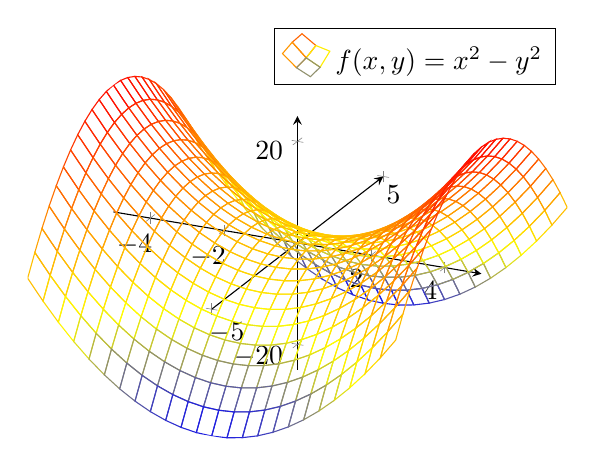
\begin{tikzpicture}
	\begin{axis} [axis lines=middle]
	\addplot3[mesh,colormap/hot, domain=-5:5]{x^2-y^2};\addlegendentry{$f(x,y)=x^2-y^2$}
	%\addplot3 ({0},{0},{0}); \addlegendentry{$(0,0,0)$}
	\end{axis}
	\end{tikzpicture}
	\end{center}
	Punto de silla en $f(0,0)=0$.
\end{figura}

\begin{proposicion} Una aplicación del \textit{teorema de Taylor} es que nos aporta información sobre cuando un punto crítico es punto de extremo relativo.\\
Sea $U\subset\R^n$ abierto, sea $\function{f}{U}{\R}$, con $f\in C^2(U)$ y sea $a\in U$. Si $a$ es punto crítico de $f$ ($df(a)=0$), tenemos (si $B(a,r)\subset U$) que $\forall x\in B(a,r)\ \exists c_x\in[a,x]\talque f(x)=\\
=\underset{P_{1,a}(x-a)}{\underbrace{f(a)+df(a)(x-a)}}+\underset{R_{1,a}(x-a)}{\underbrace{\dfrac{1}{2!}\left(\stackbin[i,j=1]{n}\sum(x_i-a_i)(x_j-a_j)D_{ij}f(c_x)\right)}}\overset{df(a)=0}=\\
=f(a)+\dfrac{1}{2!}\left(\stackbin[i,j=1]{n}\sum(x_i-a_i)(x_j-a_j)D_{ij}f(c_x)\right)\implies\\
\implies f(x)-f(a)=\dfrac{1}{2!}\left(\stackbin[i,j=1]{n}\sum(x_i-a_i)(x_j-a_j)D_{ij}f(c_x)\right)$.\\
Si $a$ es punto de máximo relativo de $f$, entonces $\exists\delta>0\ (\delta\leq r)\talque f(x)-f(a)\leq 0\\
\forall x\in B(a,\delta)$. Y por tanto, $\stackbin[i,j=1]{n}\sum (x_i-a_i)(x_j-a_j)D_{ij}f(c_x)\leq 0\ \forall x\in B(a,\delta)$. Y así, como $D_{ij}f$ e continua en $a$ tenemos que $\stackbin[i,j=1]{n}\sum (x_i-a_i)(x_j-a_j)D_{ij}f(a)\leq 0$ puesto que $c_x\overset{x\to a}\longrightarrow a$. Tenemos ahora:\\
$\stackbin[i,j=1]{n}\sum h_ih_jD_{ij}f(a)\leq 0$ con $\norm{h}<\delta$. Y de aquí deducimos que $\stackbin[i,j=1]{n}\sum (th_i)(th_j)D_{ij}f(a)=\\
=t^2\left(\stackbin[i,j=1]{n}\sum h_ih_jD_{ij}f(a)\right)\leq 0\ \forall t\in\R\implies\stackbin[i,j=1]{n}\sum h_ih_jD_{ij}f(a)\leq 0\ \forall h\in\R^n$.
\end{proposicion}

\begin{defi} La matriz $\begin{pmatrix}
	D_{11}f(a) & D_{21}f(a) & \ldots & D_{n1}f(a)\\ D_{12}f(a)& \ddots & &\vdots\\ \vdots & & \ddots & \vdots\\ D_{1n}f(a)& \ldots & \ldots & D_{nn}f(a)\end{pmatrix}$ es la matriz de derivadas parciales segundas de $f$ en $a$. La denominamos matriz \textit{Hessiana} de $f$ en $a$ y la denotamos por $H_f(a)=(D_{ij}f(a))^n_{i,j=1}$.
\end{defi}

\begin{observacion}\ \\
$\stackbin[i,j=1]{n}\sum h_ih_jD_{ij}f(a)=\begin{pmatrix} h_1 & h_2 &\ldots & h_n\end{pmatrix}
\begin{pmatrix}	D_{11}f(a) & D_{21}f(a) & \ldots & D_{n1}f(a)\\ D_{12}f(a)& \ddots & &\vdots\\ \vdots & & \ddots & \vdots\\ D_{1n}f(a)& \ldots & \ldots & D_{nn}f(a)\end{pmatrix}
\begin{pmatrix} h_1 \\ h_2 \\ \vdots \\ h_n\end{pmatrix}$
\end{observacion}

\begin{nota} Antes de continuar conviene leer el Apéndice \textsc{B. Repaso de formas cuadráticas}.\end{nota}

\begin{proposicion} Sea $U\subset\R^n$ abierto, sea $\function{f}{U}{\R}$, $f\in C^2(U)$ y sea $a\in U$ punto crítico de $f$. Entonces:
\begin{enumerate}[1)]
\item $a$ es punto de máximo relativo$\implies Q_{H_f(a)}$ es semidefinida negativa.
\item $a$ es punto de mínimo relativo$\implies Q_{H_f(a)}$ es semidefinida positiva.
\item $Q_{H_f(a)}$ es indefinida$\implies a$ es punto de silla.
\end{enumerate}
El recíproco no se cumple.
\end{proposicion}

\begin{proposicion} Sea $U\subset\R^n$ abierto, sea $\function{f}{U}{\R}$, $f\in C^2(U)$ y sea $a\in U$ punto crítico de $f$. Entonces:
\begin{enumerate}[1)]
\item Si $Q_{H_f(a)}$ es definida negativa $\implies a$ es punto de mínimo relativo.
\item Si $Q_{H_f(a)}$ es definida positiva $\implies a$ es punto de máximo relativo.\end{enumerate}
\begin{proof} Veamos lo que ocurre cuando $Q_{h_f(a)}$ es definida positiva.\\
Sea $\lambda>0$ y $\exists u\in S_{\R^n}$ de manera que $Q_{H_f(a)}(u)\geq\lambda>0$. Entonces, si $f\in C^2(U)$, sea $a\in U$ y tomando $\varepsilon_0=\dfrac{\lambda}{2n^2}$, entonces $\exists\delta_\lambda>0$ tal que $|D_{ij}f(x)-D_{ij}f(a)|<\varepsilon_0\\\forall x\in B(a,\delta_\lambda)\ \forall i,j\in\{1,2,...,n\}$. Hemos elegido de esta forma $\varepsilon_0$ por lo siguiente:\\
$Q_{H_f(x)}(u)=\stackbin[i,j=1]{n}\sum u_iu_jD_{ij}f(x)=\stackbin[i,j=1]{n}\sum u_iu_j(D_{ij}f(x)-D_{ij}f(a))+Q_{H_f(a)}(u)\geq$\\
$\geq Q_{H_f(a)}(U)-\stackbin[i,j=1]{n}\sum |u_i||u_j||D_{ij}f(x)-D_{ij}f(a)|\geq \lambda-n^2\varepsilon_0=\lambda-\dfrac{\lambda}{2}=\dfrac{\lambda}{2}>0$\\
En definitiva, hemos probado que si $\exists u\in \R^n$ con $\norm{u}=1\talque Q_{H_f(a)}(u)\geq \lambda$, entonces $\exists\delta>0\talque Q_{H_f(x)}(tu)\geq 0\ \forall t\in \R\setminus\{0\},\ \forall x\in B(a,\delta)$.\\
Ahora, si $a$ es punto crítico de $f$, por el \textit{teorema de Taylor}, $\forall x\in[a,a+\delta u],\ \exists c_x\in[a,x]$ tal que:\\
$f(x)-f(a)=\dfrac{1}{2}\stackbin[i,j=1]{n}\sum(x_i-ai)(x_j-a_j)D_ijf(c_x)=\dfrac{1}{2}Q_{H_f(c_x)}(x-a)\geq 0$.\\
Y por tanto $f(x)\geq f(a)\ \forall x\in[a,a+\delta u]$.
Ahora, si $Q_{H_f(a)}$ es definida positiva, podemos elegir $\lambda=\min\{Q_{H_f(a)}(u)\talque u\in S_{\R^n}\}>0$ y por lo anterior $\exists\delta>0\talque f(x)\geq f(a)\ \forall x\in[a,a+\delta u]\forall u\in S-{\R^n}$ y entonces $f(x)\geq f(a)\ \forall x\in B(a,\delta)$. Luego $a$ es punto de mínimo relativo.\\
La demostración es análoga para puntos de máximo relativo.
\end{proof}
\end{proposicion}

\begin{ejem} Hallar los extremos relativos de $f(x,y)=2y^2-x(x-1)^2$.\\
Tenemos $\doubleleft{D_1f=(x-1)(1-3x)}{4y}\implies$ Son puntos críticos las soluciones del sistema $\doubleright{(x-1)(1-3x)=0}{4y=0}\doubleright{x=1,y=0}{x=1/3,y=0}$\\
Tenemos que $H_f(x,y)=\begin{pmatrix}-6x+4&0\\0&4\end{pmatrix}\doubleleft{H_f(1,0)=\begin{pmatrix}-2&0\\0&4\end{pmatrix}\mathrm{\ punto\ de\ silla}}
{H_f(1/3,0)=\begin{pmatrix}2&0\\0&4\end{pmatrix}\mathrm{\ punto\ de\ minimo\ relativo}}$
\end{ejem} %Extremos relativos
	\chapter{Teoremas de la función inversa e implícita}
\section{Teorema de la función inversa}

\begin{teor} Teorema de la función inversa.\\
	Sea $U\subset\R^n$ abierto, sea $\function{f}{U}{\R^n}$, $f\in C^1(U)$ y sea $a\in U$. Si $\det(J_f(a))\neq 0$, entonces $\exists V$ abierto $\talque a\in V\subset U$ tal que:
	\begin{enumerate}[1)]
	\item $f|_{_V}$ es inyectiva y $W:=f(V)$ es un abierto.
	\item La función $\function{g=(f|_{_V})^{-1}}{W}{V}$ es $C^1$ en $W$.
	\end{enumerate}
	Además, si $f\in C^k(U)$, entonces $g\in C^k(W)$.
	\end{teor}
	
	\begin{observacion} Antes de proseguir con la demostración, veamos los siguientes comentarios al respecto.
	\begin{enumerate}[1)]
	\item $f\in C^1$ con $\det(J_f(x))\neq 0\ \forall x\in U\nimplies f$ inyectiva en $U$ si $n\geq 2$.
	\begin{ejem} Sea $f(x,y)=(e^x\cos y,e^x\sen y),\function{f}{\R^2}{\R^2},\ f\in C^\infty(\R^2)$.\\
	$J_f(x,y)=\begin{pmatrix}e^x\cos y&-e^x\sen y\\e^x\sen y&e^x\cos y\end{pmatrix}\implies\det(J_f(x,y))=e^{2x}>0\ \forall(x,y)\in\R^2$.\\
	Pero $f$ no es inyectiva pues $f(0,0)=f(0,2\pi)=(1,0)$.
	\end{ejem}
	\item Por la \textit{regla de la cadena}, como $(g\circ f)(x)=x\ \forall x\in V\y f$ es diferenciable en $a$ y $g$ es diferenciable en $f(a)$, tenemos que:\\
	$\mathrm{id}=d(g\circ f)(a)=dg(f(a))\circ df(a)\implies dg(f(a))=(df(a))^{-1}\y J_g(f(a))=(J_f(a))^{-1}$.
	\item Es necesario que $f$ sea $C^1$, no es suficiente con que sea sólo diferenciable.
	\begin{ejem} En $\R$ hay funciones con derivada positiva en un punto que no son inyectivas en ningún entorno de ese punto.\\
	En $f(x)=\doubleleft{\frac{x}{2}+x^2\sen\frac{1}{x},\ \ \ \mathrm{si\ }x\neq 0}{0,\ \ \ \mathrm{si\ }x= 0}$ es derivable en $x=0\y f'(0)=\frac{1}{2}$, pero $\nexists r>0\talque f$ sea inyectiva en $(-r,r)$.
	\end{ejem}
	\end{enumerate}
	\end{observacion}
	
	\begin{proof} Demostración del \textit{teorema de la función inversa}.
	Lo haremos en 4 pasos, dividiéndolo en las siguientes proposiciones.
	\begin{enumerate}[1)]
	\item $\exists V$ entorno abierto de $a$ tal que $f|_{_V}$ es inyectiva y $\det(J_f(x))\neq 0\ \forall x\in V$.
	\item $W:=f(V)$ es abierto.
	\item $\function{g:=(f|_{_V})^{-1}}{W}{V}$ es diferenciable en $W$.
	\item $g\in C^k(W)$ siempre que $f\in C^k(U)$.
	\end{enumerate}
	\begin{proposicioni} Sea $U\subset\R^n$ abierto,\\
	sea $\function{f}{U}{\R^n},\ f\in C^1(U)$ y sea $a\in U\talque \det (J_f(a))\neq 0$. Entonces $\exists V\subset U$ entorno abierto de $a$ tal que $f|_{_V}$ es inyectiva y $\det(J_f(x))\neq 0\ \forall x\in V$.
	\begin{proof}\ \\
	La aplicación $\xfunction{\Phi}{U}{\R}{x\to\det(J_f(x))}$ es una función continua en $U$. Como $\Phi(a)\neq 0,\ \exists r_0>0\talque \Phi(x)\neq 0\\
	\forall x\in B(a,r_0)$.\\
	$f\in C^1(U)\implies f$ es diferenciable en $U\y \function{df}{U}{\mathfrak{L}(\R^n,\R^n)}$ es continua.\\
	Como $\det(J_f(a))\neq 0\implies \function{df(a)}{\R^n}{\R^n}$ es invertible. Llamemos $L=df(a)$.\\
	Consideremos la función $\varphi(x)=f(x)-f(a)-L(x-a)\ \forall x\in U$. Tenemos que $\varphi(x)=\\
	=f(x)-f(a)-L(x)+L(a)=f(x)-L(x)+\cte\ \forall x\in U$.\\
	Como $\varphi\in C^1(U)\implies d\varphi(x)=df(x)-(dL)(x)=df(x)-L\ \forall x\in U$. En particular $d\varphi(a)=df(a)-L=L-L=0$. Tenemos ahora:\\
	$\doubleright{\varphi(x)=f(x)-f(a)-L(x-a)}{\varphi(y)=f(y)-f(a)-L(y-a)}\implies\varphi(x)-\varphi(y)=f(x)-f(y)-L(x-y)\implies\\
	\implies f(x)-f(y)=\varphi(x)-\varphi(y)+L(x-a)$.\\
	Como $d\varphi$ es continua en $a$, para $\varepsilon_0=\dfrac{1}{2\norm{L-1}}>0,\ \exists r>0$ (con $r<r_0$) tal que\\
	$\norm{d\varphi(x)-d\varphi(a)}=\norm{d\varphi(x)-0}=\norm{d\varphi(x)}<\varepsilon_0\ \forall x\in B(a,r)$.\\
	Así, como $B(a,r)$ es conexo, $\forall x,y\in B(a,r)$ por el \textit{teorema de los incrementos finitos} tenemos $\norm{\varphi(x)-\varphi(y)}\leq \left(\underset{z\in[x,y]}\sup\norm{d\varphi(z)}\right)\norm{x-y}\leq \varepsilon_0\norm{x-y}$.\\
	Veamos además que $\norm{h}=\norm{L^{-1}(L(h))}\leq\norm{L^{-1}}\norm{L(h)}\ \forall h\in \R^n$.\\
	Ahora, si $x,y\in B(a,r)$ tenemos $\norm{f(x)-f(y)}=\norm{\varphi(x)-\varphi(y)-L(x-a)}\geq\\
	\norm{2(x-y)}-\norm{\varphi(x)-\varphi(y)}\geq\dfrac{1}{\norm{L^{-1}}}\norm{x-y}-\varepsilon_0\norm{x-y}=\dfrac{1}{2\norm{L^{-1}}}\norm{x-y}>0\implies\implies f$ inyectiva en $B(a,r)\implies f$ inyectiva en $V$.
	\end{proof}
	\end{proposicioni}\ \\
	\begin{proposicioni} Sea $V\subset\R^n$ abierto,\\
	sea $\function{f}{V}{\R^n},\ f\in C^1(V)$, inyectiva en $V$ y con $\det(J_f(x))\neq 0\ \forall x\in V$, entonces $f$ es abierto, (esto es $f(G)$ abierto $\forall G\in V$, $G$ abierto).
	\begin{proof}\ \\
	Sea $G\subset V,\ G$ abierto, queremos probar que $f(G)$ es abierto.\\
	Sea $y_0\in f(G)$ tenemos que demostrar que $\exists r>0 \talque B(y_0,r)\subset f(G)$. Como $y_0\in f(G)\implies\implies\exists x_0\in G\talque f(x_0)=y_0$. $x_0\in G\y G$ abierto$\implies\exists r_0>0\talque B(x_0,r)\subset G$.\\
	Tomemos ahora $r'\in(0,r_0)$, entonces $\overline{B}(x_0,r')\subset B(x_0,r_0)\subset G$.\\
	La función $\varphi(x)=\norm{f(x)-y_0}$ es continua $\forall x\in G$, y sea $S_{x_0,r'}=\{x\in\R^n\talque\norm{x-x_0}=r'\}$ es un compacto, luego $\exists x_1\in S_{x_0,r'}\talque\norm{f(x_1)-y_0}=\varphi(x_1)=\underset{x\in S_{x_0,r'}}\min \varphi(x)=\\=\underset{x\in S_{x_0,r'}}\min\norm{f(x)-y_0}$.\\
	$\doubleright{x_0\neq x_1}{f\ \mathrm{inyectiva}}\implies f(x_0)\neq f(x_1)\implies\varphi(x_1)>0$. Tomemos ahora $r=\dfrac{\varphi(x_1)}{2}>0$, comprobemos que $B(y_0,r)\subset f(G)$.\\
	Sea $y\in B(y_0,r)\implies\norm{y-y_0}<r$. Definimos $\Phi(x)=\norm{f(x)-y}\ \forall x\in\overline{B}(x_0,r')$, entonces $\Phi$ es continua y $\overline{B}x_0,r'$ es compacto, luego $\Phi$ alcanza el mínimo en un punto $c\in\overline{B}(a,r')$. Veamos que $c\notin Fr(\overline{B}(x_0,r'))=S_{x_0,r'}$:\\
	Si $\norm{x-x_0}=r'$ entonces $\Phi(x)=\norm{f(x)-y}=\norm{f(x)-y_0+y_0-y}\geq\\
	\geq\norm{f(x)-y_0}-\norm{y_0-y}>\varphi(x_1)-\norm{y_0-y}>\varphi(x_1)-r=\dfrac{\varphi(x_1)}{2}=r>\norm{y-y_0}=\\=\norm{y-f(x_0)}\geq\norm{y-f(c)}=\Phi(c)$.\\
	Luego $c\in\mathring{\overline{B}}(x_0,r')=B(x_0,r')$. Ahora:\\
	$\doubleright{\Phi>\geq 0}{\Phi(c)\leq\Phi(x)\ \forall x\in\overline{B}(x_0,r')}\implies \Phi^2(c)\leq\Phi^2(x)\ \forall x\in\overline{B}(x_0,r')$.\\
	Como $\Phi^2$ tiene un mínimo relativo en el punto $c$ perteneciente al interior de $\overline{B}(x_0,r')\y\Phi^2$ es diferenciable en $c$, tenemos que $\gradiente\Phi^2(c)=\overline{0}\in\R^n$.\\
	Como $\Phi^2(x)=\norm{f(x)-y}^2=\stackbin[i=1]{n}\sum(f_i(x)-y_i)^2\implies \overline{0}=(0,0,...,0)=\gradiente\Phi^2(c)=\\
	=(D_1\Phi^2(c),D_2\Phi^2(c),...,D_n\Phi^2(c))=\\
	=\left(\stackbin[i=1]{n}\sum2(f_i(c)-y_i)D_1f_i(c),...,\stackbin[i=1]{n}\sum2(f_i(c)-y_i)D_nf_i(c)\right)=\stackbin[i=1]{n}\sum2(f_i(c)-y_i)\gradiente f_i(c)$.\\
	Tenemos así una combinación lineal de vectores $\gradiente f_i(c)$ (cuyas coordenadas son las filas de la matriz) y como $\det(J_f(c))\neq 0$, esos vectores son lienalmente independientes. Como esa combinación lineal es $\overline{0}$, sus coeficientes han de ser todos $0$, es decir,\\
	$2(f_i(c)-y_i)=0\ \forall 1\leq i\leq n$. Con lo cual $f(c)=(f_1(c),f_2(c),...,f_n(c))=y=(y_1,y_2,...,y_n)$. Por tanto $y\in f(B(x_0,r'))\subset f(G)$.
	\end{proof}
	\end{proposicioni}
	
	\begin{proposicioni} Sean $V,W\subset\R^n$ abiertos, sea $\function{f}{V}{W}$ biyectiva con inversa $\function{g}{W}{V}$ continua en $W$. Si $f$ es diferenciable en $x_0\in V\y\det(J_f(x_0))\neq 0$ entonces $g$ es diferenciable en $f(x_0)$.
	\end{proposicioni}
	\begin{proof}\ \\
	$f$ es diferenciable en $x_0$ y $\det(J_f(x_0)\neq 0\implies L:=df(x_0)$ es invertible; queremos probar que $L^{-1}=dg(f(x_0))$ o equivalentemente, que $\dfrac{g(f(x_0)+k)-g(f(x_0))-L^{-1}(k)}{\norm{k}}\overset{k\to 0}\longrightarrow 0$.\\
	Sabemos por hipótesis que $\dfrac{f(a+h)-f(a)-L(h)}{\norm{h}}\overset{\htiende}\longrightarrow0$. Definamos:\\
	$\varphi(h):=\doubleleft{\dfrac{f(a+h)-f(a)-L(h)}{\norm{h}},\ \mathrm{si\ }h\neq0\ (a+h\in V)}{0,\ \mathrm{si\ }h=0}$\\
	Tenemos que $\varphi$ es continua en 0. $\forall k\neq0\talque f(x_0)+k\in W$ llamamos\\
	$h(k)=\boxed{g(f(x_0)+k)-x_0}$\textbf{(*)}($=g(f(x_0)+k)-g(f(x_0))$\ ). Como $f$ es inyectiva y por tanto $g$, tenemos que si $k\neq0\implies h(k)\neq 0$. Además, como $g$ es continua en $f(x_0)$,\\
	$\limite{h(k)}{\ktiende}=\limite{}{\ktiende}(g(f(x_0)+k)-g(f(x_0)))=0$, y por la continuidad de $\varphi$ en $0$, tenemos $\limite{}{\ktiende}\varphi(h(k))=\varphi(0)=0$.\\
	Por \textbf{(*)}, $h(k)+x_0=g(f(x_0)+k)\implies f(h(k)+x_0)=f(g(f(x_0+k))=f(x_0)+k\implies\\
	\implies\boxed{k=f(x_0+h(k))-f(x_0)}$\textbf{(**)}.\\
	Así, si $k\neq 0\talque f(x_0)+k\in W$, tenemos:\\
$	\dfrac{g(f(x_0)+k)-g(f(x_0))-L^{-1}(k)}{\norm{k}}=\dfrac{h(k)-L^{-1}(k)}{\norm{k}}\overset{\textbf{(**)}}=\dfrac{h(k)-L^{-1}(f(x_0+h(k))-f(x_0))}{\norm{k}}=\\
=\dfrac{h(k)-L^{-1}(\ \norm{h(k)}\varphi(h(k))+L(h(k))\ )}{\norm{k}}=\dfrac{h(k)-\norm{h(k)}L^{-1}(\varphi(h(k)))-L^{-1}(L(h(k)))}{\norm{k}}=\\
=\dfrac{\norm{h(k)}}{\norm{k}}L^{-1}(\varphi(h(k)))$. Como $\limite{}{\ktiende}L^{-1}(\varphi(h(k)))=L^{-1}(\varphi(0))=L^{-1}(0)=0$, sólo nos queda probar que $\dfrac{\norm{h(k)}}{\norm{k}}$ está acotado en un entorno de $k=0$.\\
Como $\norm{k}=\norm{f(x_0+h(k))-f(x_0)}=\norm{\norm{h(k)}\varphi(h(k))+L(h(k))}=\\
=\norm{h(k)}\norm{\varphi(h(k))+L\left(\dfrac{h(k)}{\norm{h(k)}}\right)}\geq\norm{h(k)}\left(\norm{L\left(\dfrac{h(k)}{\norm{h(k)}}\right)}-\norm{\varphi(h(k))}\right)\implies\\
\implies\dfrac{\norm{h(k)}}{\norm{k}}\leq\dfrac{1}{\norm{L\left(\dfrac{h(k)}{\norm{h(k)}}\right)}-\norm{\varphi(h(k))}}$. Como $L$ es invertible y continua:\\
$\underset{u\in S_{\R^n}}\min\norm{L(u)}=\norm{L(u_0)}=\alpha>0$, y como $\limite{\varphi(h(k))}{\ktiende}=0$, para $\varepsilon_0=\dfrac{\alpha}{2}>0,\\
\exists\delta>0\talque \norm{\varphi(h(k))}<\varepsilon_0=\dfrac{\alpha}{2}\ \forall k\in B(0,\delta)$. Luego $\dfrac{\norm{h(k)}}{\norm{k}}\leq\dfrac{1}{L\left(\dfrac{h(k)}{\norm{h(k)}}\right)-\norm{\varphi(h(k))}}\leq\\
\leq\dfrac{1}{\alpha-\dfrac{\alpha}{2}}=\dfrac{2}{\alpha}\ \forall k\in B(0,\delta)\setminus\{0\}\implies \dfrac{\norm{h(k)}}{\norm{k}}$ está acotado en un entorno de $k=0\implies\\
\implies \limite{}{\ktiende}\dfrac{g(f(x_0)+k)-g(f(x_0))-L^{-1}(k)}{\norm{k}}=0\implies g$ es diferenciable en $f(x-0)$.
	\end{proof}
	
	\begin{proposicioni} Sean $V\y W\subset\R^n$ abiertos, sea $\function{f}{V}{W}$ biyectiva, diferenciable $V$, con $\det(J_f(x))\neq0\ \forall x\in V\y$con\\
	$\function{g:=f^{-1}}{W}{V}$ continua en $W$. Si $k\in \N\y f\in C^k(V)$, entonces $g\in C^k(W)$.
	\end{proposicioni}
	\begin{proof}\ \\
	Por la \textit{proposición 3} $g$ es diferenciable en $W$ y por la \textit{regla de la cadena}, $dg(f(x))=(df(x))^{-1}\\
	\forall x\in V$ (pues $\id_V=(f\circ g)$). O escrito de otra forma, $dg(y)=(df(g(y))^{-1}\ \forall y\in W$ con lo cual $J_g(y)=(J_f(g(y)))^{-1}$.\\
	Podemos identificar cada elemento de la matriz $n\times n$ con un elemento de $\R^{n^2}$. El conjunto $\mathcal{U}=\left\{(a_{ij})_{i,j=1}^n\talque \det\left((a_{ij})_{i,j=i}^n\right)\neq0\right\}\subset\R^{n^2}$ es un abierto de $\R^{n^2}$, pues la aplicación $\xfunction{\det}{\R^{n^2}}{\R}{(a_{ij})_{i,j=1}^n\to\\det\left((a_{ij})_{i,j=i}^n\right)}$ es un polinomio, por lo tanto continuo, $\mathcal{U}=\det^{-1}((-\infty,0)\cup(0,+\infty))$ y $((-\infty,0)\cup(0,+\infty))$ es un abierto de $\R$, por tanto $\mathcal{U}$ es abierto.\\
	La aplicación $\xfunction{\phi}{\mathcal{U}}{\mathcal{U}}{A=(a_{ij})^n_{i,j=1}\to A^{-1}}$ es $C^\infty$ en $\mathcal{U}$, pues cada componente es un cociente de polinomios cuyo denominador no se anula nunca.\\
	Llamemos $J_f$ a la función $\xfunction{J_f}{V}{\R^{n^2}}{x\to J_f(x)}$ y para cada $1\leq i,j\leq n$ llamemos $\xfunction{\Pi_{ij}}{\R^{n^2}}{\R}{(a_{kl})_{k,l=1}^n\to a_{ij}}$. Tenemos que $\Pi_{ij}\in C^\infty(\R^{n^2})$.\\
	$\forall 1\leq i,j\leq n$ tenemos que $D_jg_i$ es $D_jg_i\colon\underset{y}W\stackbin[\longrightarrow]{g}\longrightarrow\underset{g(y)}V\stackbin[\longrightarrow]{J_f}\longrightarrow\underset{J_f(g(y))}{\mathcal{U}}\stackbin[\longrightarrow]{\Phi}\longrightarrow\underset{(J_f(g(y)))^{-1}}{\mathcal{U}}\stackbin[\longrightarrow]{\Pi_{ij}}\longrightarrow\underset{\Pi_{ij}((J_f(g(y)))^{-1})}\R$ y $\Pi_{ij}\left((J_f(g(y)))^{-1}\right)=\Pi_{ij}(J_g(y))=D_jg_i(y)$, o sea:\\
	$D_jg_i=\Pi_{ij}\circ\Phi\circ J_f\circ g$. Ahora si $f\in C^1(V)$ entonces $J_f$ es continua  y por tanto (por ser $g$ continua y $\Phi,\Pi_{ij}$ son $C^\infty$) tenemos que $D_jg_i$ es continua en $W$.\\
	$D_jg_i$ continua en $W\ \forall i,j\in\{1,2,...,n\}\iff g\in C^1(W)$.\\
	Ahora si $f\in C^2(V)\implies \doubleleft{f\in C^1(V)\implies g\in C^1(W)}{J_f\in C^1(V)}$\\
	$g,J_f,\Phi\y\Pi_{ij}$ son $C^1$, luego $D_jg_i$ es $C^1(W)\y $ si $D_jg_i\C^1(W)\ \forall i,j\in\{1,2,...,n\}\implies$\\
	$\implies g\in C^2(W)$ y por inducción sobre $k$ tenemos que si $f\in C^k(V)\implies g\in C^k(W)$.
	\end{proof}
	
	\textbf{Demostramos ahora el \textit{teorema de la función inversa.}}\\
	Por la \textit{proposición 1}, $\exists	V$ entorno abierto de $a$, $V\subset U\talque f|_{_V}$ es inyectiva y $J_f(x_0)\neq 0\\\forall x\in V$. Por la \textit{proposición 2}, sea $W:=f(V)$ abierto y $f|_{_V}$ es abierto por lo que $\function{g:=(f\_{_V})^{-1}}{W}{V}$ es continua. Por la \textit{proposición 3} $g$ es diferenciable en $W$ y por la \textit{proposición 4}, como $f\in C^1(U)$, tenemos que $g\in C^1(W)$ y además si $f\in C^k(U)\implies\\\implies g\in C^k(W)$.
	\end{proof}
	
	\begin{observacion} De las \textit{proposiciones 1} y \textit{2} se deduce fácilmente lo siguiente:\\
	Sea $U\subset \R^n$ abierto, sea $\function{f}{U}{\R^n},\ f\in C^1(U)$ con $\det(J_f(x))\neq 0\ \forall x\in U$. Entonces $f$ es abierto (\textit{Teorema de la aplicación abierta)}.
	\end{observacion}
	
	\begin{defi} Un difeomorfismo entre dos abiertos $U\y W$ de $\R^n$ es una aplicación biyectiva $\function{f}{V}{W}$ tal que $f\y f^{-1}$ son diferenciables y, además, si $f\y f^{-1}$ son de clase $k$, diremos que $f$ (ó $f^{-1}$) es un $C^k$-difeomorfismo entre $V\y W$.\\
	El \textit{teorema de la función inversa} nos dice que si $\function{f}{V}{W}$ es una aplicación biyectiva entre dos abiertos $V\y W\subset\R^n$, entonces la condición necesaria y suficiente para que $f$ sea $C^1-$difeomorfismo es que $\det(J_f(x))\neq0\ \forall x\in V$.\\
	A los difeomorfismos se les llama a veces \textit{cambios de variable} o \textit{aplicaciones regulares}.\\
	Diremos que $f$ es un difeomorfismo local en $a$ si existe un entorno abierto $V$ de $a$ tal que $f|_{_V}$ es difeomorfismo sobre su imagen.
	\begin{ejem} Ejemplo de difeomorfismo:
	\[\xfunction{f}{(0,+\infty)\times(0,2\pi)}{\R^2\setminus\{(x,0)\talque x\geq0\}}{\ \ \ \ \ \ \ \ \ \ \ (\rho,\theta)\ \longrightarrow\ (\rho\cos\theta,\rho\sen\theta)}\]
	\end{ejem}
	\end{defi}
	
	\section{Teorema de la función implícita}
	
	\begin{teor} Teorema de la función implícita en $\R^2$.\\
Sea $U\subseteq \R^2$ abierto y sea $\function{F}{U}{\R}$ de clase $C^1$ en $U$ y sea $(x_0,y_0)\in U\talque F(x_0,y_0)=0$. Si $\dfrac{\partial F}{\partial y}(x_0,y_0)\neq 0$ entonces existe un entrono abierto $V$ de $(x_0,y_0)$, existe un entorno abierto $A\subseteq\R$ de $x_0$ y existe una única función $\function{f}{A}{\R}$ tal que $F(x,f(x))=0\ \forall x\in A$ $(\y \{(x,y)\in V\talque F(x,y)=0\}=\{(x,f(x))\talque x\in A\})$. Además, $f$ es $C^1$ en $A$. Más aún, si $F\in C^k(U)$, $f\in C^k(A)$.
\end{teor}

\begin{ejem} La ecuación $x^2+y^2=1$ define a $y$ como función implícita de $x$ en un entorno de $(0,1)$.\\
Sea $F(x,y)=x^2+y^2-1,\ F\in C^\infty(\R^2)$. Tenemos $x^2+y^2=1\iff F(x,y)=0$.\\
Así, $(0,1)$ es solución, pues $F(0,1)=0^2+1^2-1=0\y \dfrac{\partial F}{\partial y}(0,1)=2y|_{_{(0,1)}}=2\neq 0$. Luego $\exists V$ entorno abierto de $(0,1)$, $\exists I\subset\R$ intervalo abierto que contiene a $0$ y $\exists\function{f}{I}{\R},\ C^\infty$ en $I\talque$ $\{(x,y)\in V\talque F(x,y)=0\}=\{(x,f(x))\talque x\in I\}$.
\end{ejem}

\begin{defi} Sea $U\subset\R^{n+m}$ abierto y sea $\function{F}{U}{\R^m}$, diremos que la ecuación $F(x,y)=0$ con $x=(x_1,x_2,...,x_n)\y y=(y_1,y_2,...,y_m)$, define a la variable $y$ como función implícita de la variable $x$ en un entorno de solución $(a,b)$ (o sea, $F(a,b)=0$) si existe un entorno abierto $V\subset\R^{n+m}$ de $(a,b)$, existe un entorno abierto $A\subset\R^n$ de $x_0$ y existe una función $\function{f}{A}{\R^m}$ tal que $\{(x,y)\in V\talque F(x,y)=0\}=\{(x,f(x))\talque x\in A\}$. En particular $f(a)=b$.
\end{defi}

\begin{teor}Teorema de la función implícita.\\
Sea $U\subset\R^{n+m}$ abierto, sea $\function{F}{U}{\R^m}$ de clase $C^1$ en $U$ y sea $(a,b)=\\=(a_1,a_2,...,a_n,b_1,b_2,...,b_m)\in U$ tal que $F(a,b)=0$. Si $\det\left(\left(\dfrac{\partial F_i}{\partial y_j}\right)_{1\leq i,j\leq m}(a,b)\right)\neq 0$. Entonces la ecuación $F(x,y)=0$ (con $x=(x_1,...,x_n)\y y=(y_1,...,y_m)$) define a la variable $y$ como la función implícita de la variable $x$ en un entorno de $(a,b)$, es decir, existe\\
$V\subset\R^{n+m}$ entorno abierto de $(a,b)$, existe $A\subset\R^n$ entorno abierto de $a$ y existe \\
$\function{f}{A}{\R^m}$ tal que $\{(x,y)\in V\talque F(x,y)=0\}=\{(x,f(x))\talque x\in A\}$. Además, $f$ es $C^1$ en $A$. Más aún, si $F\in C^k(U)$, entonces $f\in C^k(A)$.
\end{teor}

\begin{proof}\ \\
Definamos $\xfunction{\Phi}{U}{\R^{n+m}}{(x,y)\to(x,F(x,y))=(x_1,...,x_n,F_1(x,y),...,F_m(x,y))}$. Como $F\in C^1(U)$ tenemos que\\
$\Phi\in C^1(U)$ y $\det(J_\Phi(x,y))=$
\[\begin{split}
=&\left|\begin{array}{c|c}
\begin{array}{cccc}
1&0&\cdots&0\\ 0&1&\ldots&0\\ \vdots&\vdots&\ddots&\vdots\\ 0&0&\cdots&1\\
\hline
D_1F_1&D_2F_1&\ldots&D_nF_1\\ D_1F_2&D_2F_2&\ldots&D_nF_n\\ \vdots&\vdots&\ddots&\vdots\\ D_1F_m&D_2F_m&\ldots&D_nF_m
\end{array} & \begin{array}{cccc}
0&0&\cdots&0\\ 0&0&\cdots&0\\ \vdots&\vdots&\ddots&\vdots\\ 0&0&\cdots&0\\
\hline
D_{n+1}F_1&D_{n+2}F_1&\ldots&D_{n+m}F_1\\ D_{n+1}F_2&D_{n+2}F_2&\ldots&D_{n+m}F_2\\
\vdots&\vdots&\ddots&\vdots\\ D_{n+1}F_m&D_{n+2}F_m&\ldots&D_{n+m}F_m
\end{array} 
\end{array}\right|
\end{split}
=\]
$=\deter{D_{n+1}F_1&D_{n+2}F_1&\ldots&D_{n+m}F_1\\ D_{n+1}F_2&D_{n+2}F_2&\ldots&D_{n+m}F_2\\
\vdots&\vdots&\ddots&\vdots\\ D_{n+1}F_m&D_{n+2}F_m&\ldots&D_{n+m}F_m}=\det\left(\left(\dfrac{\partial F_i}{\partial y_j}\right)_{1\leq i,j\leq m}(a,b)\right)\neq 0$.\\
Así, por el \textit{teorema de la función inversa} $\exists V$ entorno abierto de $(a,b)$ tal que $W=\Phi(V)$ es abierto de $\R^{n+m}\y\function{\Phi|_{_V}}{V}{W}$ es $C^1$ difeomorfismo.\\
Sea $A=\{x\in\R^n\talque(x,0)\in W\}$ abierto de $\R^n$ pues $A=h^{-1}(W)$ con $h(x)=(x,0)$.\\
$A$ es abierto y $a\in A$ (pues $(a,0)=(a,F(a,b))=\Phi(a,b)\in W$).\\
Sea $\function{g=\left(\Phi|_{_V}\right)^{-1}}{W}{V}$ con $g=(g_1,g_2,...,g_{n+m})$ definimos\\
$f(x)=(g_{n+1}(x,0),g_{n+2}(x,0),...,g_{n+m}(x,0))\ \forall x\in A$. Como $g\in C^1(W),\ h\in C^\infty(\R^n)\y\\
f(x)=(g_{n+1}(x,0),...,g_{n+m}(x,0))$ tenemos que $f\in C^1(A)$. Más aún, si $F$ es $C^k(U)$ entonces $g$ también lo es y por lo tanto $f\in C^k(A)$.\\
Probemos ahora que $\{(x,y)\in V\talque f(x,y)=0\}=\{(x,F(x))\talque x\in A\}$.
\begin{itemize}
\item Probemos $\{(x,y)\in V\talque F(x,y)=0\}\subset\{(x,f(x))\talque x\in A\}$\\
Si $(x,y)\in V\y F(x,y)=0\implies\doubleleftright{\Phi(x,y)\in W}{\Phi(x,y)=(x,F(x,y))=(x,0)}\implies\\ \implies (x,0)\in W\implies x\in A$.\\
Por otro lado, si $(x,y)\in V,\ (x,y)=g(\Phi(x,y))=g(x,F(x,y))=g(x,0)=\\=(g_1(x,0),...,g_n(x,0),g_{n+1}(x,0),...,g_{n+m}(x,0))=\\=(x_1,x_2,...,x_n,f_1(x),f_2(x),...,f_m(x))=(x,f(x))$. Luego $(x,y)=(x,f(x))$ con $x\in A$.
\item Probemos $\{(x,y)\in V\talque F(x,y)=0\}\supset\{(x,F(x))\talque x\in A\}$\\
Si $x\in A$, probemos que $(x,f(x))\in V\y F(x,f(x))=0$.\\
$x\in A\iff(x,0)\in W\implies g(x,0)\in V\y g(x,0)=(x,f(x))\in V$. Para acabar, $(x,0)\in W\implies(x,0)=\Phi(g(x,0))=\Phi(x,f(x))=(x,F(x,f(x)))\implies\\\implies F(x,f(x))=0$.
\end{itemize}
\end{proof}

\begin{observacion} El hecho de que $\{(x,y)\in V\talque F(x,y)=0\}=\{(x,f(x))\talque x\in A\}$ nos dice:
\begin{enumerate}[1)]
\item Para cada $x\in A\ \exists!y\talque (x,y)\in V\y F(x,y)=0$. Ese $y$ es justo al que llamamos $f(x)$.
\item Como $(a,b)\in V\y F(a,b)=0$ entonces $b=f(a)$.
\item $F(x,f(x))=0\ \forall x\in A$.
\end{enumerate}
Esto nos dice que la función $h(x)=F(x,f(x))$ es idénticamente nula en $A$ (entorno de $a$), con lo cual, sus derivadas parciales de todas sus componentes valen $0$ en $a$. Esto nos permite calcular las derivadas parciales de los componentes de $f$ en $a$.
\end{observacion}

\begin{ejem} Sea $z^3+x(y-1)=1$. ¿Define $z$ como función implícita de $x$ e $y$ en un entorno de $(0,1,1)$?\\
Sea $F(x,y,z)=z^3+x(y-1)-1$,\ $F\in C^\infty(\R^3),\ \function{F}{\R^3}{\R}$.\\
Tenemos que $F(0,1,1)=0\y\dfrac{\partial F}{\partial z}=3z^2|_{_{(0,1,1)}}=3\neq 0$.\\
Luego por el \textit{teorema de la función implícita}, $\exists V$ entorno abierto de $(0,1,1)$, $\exists A\subset\R^2$ entorno abierto de $(0,1)\y\exists\function{f}{A}{\R}$ tal que $f\in C^\infty(A)$. Tenemos además que $F(x,y,f(x,y))=\ =0\ \forall (x,y)\in A,\ \{(x,y,z)\in V\talque F(x,y,z)=0\}=\{(x,y,f(x,y)\talque(x,y)\in A\}\y f(0,1)=1$.\\
$F(x,y,f(x,y))=0\ \forall(x,y)\in A$.
\end{ejem} %Teorema de la funcion inversa e implícita
	\chapter[Extremos cond. y variedades diferenciables]{Extremos condicionados y variedades diferenciables}
\section{Extremos condicionados}

\begin{defi} Sea $D\subset\R^n$, sea $\function{f}{D}{\R}$ y sea $M\subset D$. Diremos que $p\in M$ es punto de extremo relativo de $f$ condicionado a $M$ si es punto de extremo relativo de $f|_{_M}$; Es decir, $\exists r>0$ tal que, bien $f(p)\leq f(x)\ \forall x\in M\cap B(p,r)$, o bien $f(p)\geq f(x)\ \forall x\in M\cap B(p,r)$.
\end{defi}

\begin{defi} Sea $U\subset\R^n$ abierto y sea $\function{f}{U}{\R^m}$ de clase $C^1$ en $U$. Diremos que $a\in U$ es punto regular de $f$ si $\rg(J_f(a))$ es máximo.
\end{defi}

\begin{observacion} Si $n>m$, que $a$ sea punto regular de $f$ se simplifica que $\rg(J_f(a))=m$. Como $J_f(a)=\begin{pmatrix}\gradiente f_1(a)\\\gradiente f_2(a)\\\vdots\\\gradiente f_m(a)
\end{pmatrix}$ esto es equivalente a que los vectores $\gradiente f_1(a),\gradiente f_2(a),...,\gradiente f_m(a)$ sean linealmente independientes.\\
En cambio, si $n<m$, como $J_f(a)=\begin{pmatrix}D_1f_1(a)&\cdots&D_nf_1(a)\\\vdots&\ddots&\vdots\\ D_1f_m(a)&\cdots &D_nf_m(a)\end{pmatrix}$, entonces son los vectores columna los que han de ser linealmente independientes.\\
Diremos que $f$ es regular en $U$ si $f\in C^1(U)\y\rg(J_f(x))$ es máximo $\forall x\in U$.
\end{observacion}

\section{Variedades diferenciables}

\begin{observacion} Sea $U\in\R^n$ abierto. Si $\function{f}{U}{\R^m}$ es regular en $U\y n>m$ el conjunto $M=\{x\in U\talque F(x)=\overline{0}\}=\stackbin[i=1]{m}\bigcap\{x\in U\talque F_i(x)=0\}$. Cada $\{x\in U\talque F_i(x)=0\}$ es un conjunto de nivel de la función $\function{F_i}{U}{\R}$. Por tanto, si $p\in U\y \gradiente F_i(p)$ es ortogonal a $\{x\in U\talque F_i(x)=0\}$, el hiperplano tangente a este conjunto en $p$ es el que pasa por $p$ y tiene vector ortogonal $\gradiente F_i(p)$. Entonces, el espacio afín tangente a $M$ en $p$ es la intersección de los hiperplanos tangentes anteriores; Es decir, sea $H_i$ el hiperplano tangente a cada conjunto $\{x\in U\talque F_i(x)=0\}$ en $p$, el espacio afín tangente a $M$ en $p$ sería $\stackbin[i=1]{m}\bigcap H_i$.
\end{observacion}

\begin{defi} Sea $M\subset\R^n$. Diremos que $M$ es una variedad diferenciable o variedad regular de dimensión $k<n$ si se cumple alguna de las siguientes condiciones equivalentes:
\begin{enumerate}[1)]
\item $\forall p\in M,\ \exists W\subset\R^n$ entorno abierto de $p\y\exists\function{F}{W}{\R^m}$ con $m=n-k$ regular, tal que $M\cap W=\left\{x\in W\talque F(x)=\overline{0}\right\}$.
\item $\forall p\in M,\ \exists W\subset\R^n$ entorno abierto de $p=(\overset{a}{\overbrace{p_1,p_2,...p_k}},\overset{b}{\overbrace{p_{k+1},...,p_n}}),\ \exists V\in\R^k$ entorno abierto de $a\y\exists\function{g}{V}{\R^m},\ g\in C^1(V)$ tal que $M\cap W=\{(x,g(x))\talque x\in V\}$ (salvo permutación de variables).
\item $\forall p\in M,\ \exists W\subset\R^n$ entorno abierto de $p$ tal que $M\cap W$ admite una parametrización regular; Esto es, $\exists G\subset\R^k$ abierto y $\exists\function{\varphi}{G}{\R^n}$ regular tal que $\varphi(G)=M\cap W\y\\
i\circ\function{\varphi}{G}{M\cap W}$ es homeomorfismo.
\end{enumerate}
\begin{nota}El \textit{teorema de la función inversa} y el \textit{teorema de la función implícita} nos dicen que las anteriores condiciones son equivalentes.\end{nota}
\end{defi}

\begin{ejem} \ 
\begin{itemize}
\item Son variedades regulares de dimensión 1 (curvas regulares) las circunferencias, elipses, parábolas y gráficas de $\function{f}{I}{\R}$ con $f\in C^1(I)$ e $I$ intervalo abierto.
\item La hélice $\varphi(t)=(\cos t,\sin t, t)$.
\item Son variedades regulares de dimensión 2 (superficies regulares) la esfera unidad, los elipsoides y las gráficas de $\function{f}{U}{\R}$ con $f\in C^1(U)\y U\subset\R^2$ abierto.
\item $M=\{(x,y,z)\in\R^3\talque z^2=x^2+y^2\}$ (conos con vértice común en $(0,0,0)$) no es una variedad regular, pero $M\setminus\{(0,0,0)\}$ sí lo es.
\end{itemize}
\end{ejem}

\begin{proposicion} Sea $\function{F}{U}{\R^m}$ con $U\subset\R^n$ abierto y $n>m$. Si $F$ es regular en $U$ (esto es, $F\in C^1(U)\y\rg(J_f(x))$ es máximo, o sea $m$, $\forall x\in U$), entonces $M=\{x\in U\talque F(x)=\overline{0}\}$ es variedad regular.
\end{proposicion}

\begin{ejem} Sea $F(x,y,z)=x^2+y^2+z^2-1$.\\
Tenemos que $F\in C^\infty(\R^3)$. Tenemos además que $J_f(x,y,z)=\begin{pmatrix}2x&2y&2z\end{pmatrix}$ luego\\
$\rg(J_f(x,y,z))\neq 1$ (máximo) $\iff (x,y,z)=(0,0,0)$. Por lo que tenemos que $F$ es regular en $\R^3\setminus\{(0,0,0)\}$. Por último, por la proposición anterior, tenemos que $M=\{(x,y,z)\talque F(x,y,z)=0\}\subset\R^3\setminus\{(0,0,0)\}$ es una variedad regular de dimensión $3-1=2$.
\end{ejem}

\begin{proposicion} Veamos un caso particular de la proposición anterior:\\
Sea $\function{F}{U}{\R^m}$ con $U\subset\R^n abierto\y n>m$ y $F\in C^1(U)$. Sea $M=x\in U\talque F(x)=\overline{0}\}$, entonces, si cada $p\in M$ es punto regular de $F$, tenemos que $M$ es variedad regular de dimensión $n-m$.
\end{proposicion}

\begin{ejem} Sea $\function{f}{V}{\R^m}$ con $V\subset\R^k$ abierto y $\in C^1(V)$, entonces su gráfica $M=\{(x,f(x,)\talque x\in V\}\subset\R^{k+m}$ es una variedad regular de dimensión $k$.\\
En efecto, definamos $\xfunction{F}{V\times\R^m}{\R^m}{(x,y)\to(y-f(x))}$\\
Tenemos que $V\times\R^m$ es abierto en $\R^{k+m}$, $F\in C^1(V\times\R^m)\y\\
M=\{(x,y)\in V\times\R^m\talque F(x,y)=0\}$. Además si $(x,y)\in V\times\R^m$, tenemos:\\
$J_f(x,y)=\begin{pmatrix}-D_1f1(x)&-D_2f_1(x)&\cdots&-D_kf_1(x)&1&0&\cdots&0\\
-D_1f2(x)&-D_2f_2(x)&\cdots&-D_kf_2(x)&0&1&\cdots&0\\
\vdots&\vdots&\ddots&\vdots&\vdots&\vdots&\ddots&\vdots\\
-D_1fm(x)&-D_2f_m(x)&\cdots&-D_kf_m(x)&0&0&\cdots&1\\\end{pmatrix}$ y por tanto\\
$\rg(J_f(x,y))=m\ \forall(x,y)\in V\times\R^m$.
\end{ejem}

\begin{ejem} Sea $f(x,y)=x^2+y^2\ \forall (x,y)\in\R^2$, tenemos que ``gráfica de $f$''$:=\\
=\{(x,y,f(x,y))\talque (x,y)\in\R^2\}=\{(x,y,f(x,y))\talque (x,y)\in\R^2\}=\\
=\{(x,y,z)\in\R^3\talque z=x^2+y^2\}$, que es una paraboloide y es una variedad regular de dimensión 2.
\end{ejem}

\begin{ejem} Sea $M\subset\R^n$ es una variedad regular de dimensión $k<n\y M=\{x\in U\talque F(x)=0\}$ con $U\subset\R^n$ abierto y $\function{F}{U}{\R^m}$ regular en $U$ (donde $m=n-k$).\\
Fijado $p\in M$, como $\rg J_f(p)=m$, por el \textit{teorema de la función implícita} la ecuación $F(x)=0$ define a sus variables (que suponemos sin pérdida de generalidad que son las últimas) como función implícita de las $k$ primeras en un entorno de $p=(p_1,p_2,...,p_k,p_{k+1},...,p_{k+m})$; Es decir, $\exists W$ entorno abierto de $p,\ \exists V$ entorno abierto de $a\y\exists! \function{f}{V}{\R^m},\ f\in C^1(V)$ tal que $F(\oversim{x},f(\oversim{x}))=0\ \forall\oversim{x}=(x_1,x_2,...,x_k)\in V\y f(a)=b$.\\
Si definimos $\xfunction{\Phi}{V}{\R^{k+m=n}}{\oversim{x}\to(\oversim{x},f(\oversim{x}))}$, tenemos que $\Phi$ es parametrización regular de $M\cap W$ pues $\phi(V)=\{(\oversim{x},f(\oversim{x}))\talque\oversim{x}\in V\}=M\cap W$. Por último vemos que $\Phi\in C^1(V),\ \Phi$ es regular en $V\y \function{\Phi}{V}{M\cap W}$ es homeomorfismo.
\end{ejem}

\begin{observacion} Si $M\subset\R^n$ es variedad regular de dimensión $k<n\implies M\cap G$ es variedad regular de dimensión $k$ si $G$ es abierto de $\R^n$ con $M\cap G\neq\vacio$
\end{observacion}

\section{Teorema de multiplicación de Lagrange}

\begin{teor} Sea $U\subset\R^n$ abierto, sea $\function{f}{U}{\R}$ de $C^1$ en $U$ y sea $M\in U$ variedad regular de dimensión $k<n$. Si $M=\{x\in U\talque F(x)=\overline{0}\}$ para una cierta función $\function{F}{U}{\R^{n-k}}$ regular en $U$, entonces, una condición necesaria para que un punto $p\in M$ sea punto de extremo relativo condicionado de $f$ en $M$ es que \\
$\gradiente f(p)\in [\{\gradiente F_1(p),\gradiente F_2(p),...,\gradiente F_m(p)\}]$ (espacio vectorial engendrado por estos vectores); Es decir, $\exists \lambda_1,\lambda_2,...\lambda_m\in\R$ tal que $\gradiente f(p)=\stackbin[i=1]{m}\sum\lambda_i\gradiente F_i(p)$. A estos $\lambda_i$ se les llama \textit{multiplicadores de Lagrange}.
\end{teor}

\begin{proof}\ \\
Como $p$ es un punto de extremo relativo condicionado de $f$ (supongamos que $p$ es punto de máximo relativo condicionado)$\y p\in M$ es variedad regular, $\exists W\subset U,\ W$ entorno abierto de $p=(\overset{a}{\overbrace{p_1,p_2,...,p_k}},\overset{b}{\overbrace{p_{k+1},...,p_{k+m}}})=(a,b),\ \exists V$ entorno abierto de $a\y\exists!\function{g}{V}{\R^m}$ con $g\in C^1(V)$ tal que $f(x,y)\leq f(p)\ \forall (x,y)\in W\cap M$, donde $W\cap M=\{(x,g(x))\talque x\in V\}$. Tenemos así que $g(a)=b\y F(x,g(x))=0\ \forall x\in V$.\\
Así la función $\xfunction{\Phi}{V}{\R^n}{x\to(x,g(x))}$ es una parametrización regular de $M\cap W$. Tenemos\\
$f(x,y)\leq f(p)\ \forall (x,y)\in M\cap W\iff f(\Phi(x))\leq f(\Phi(a))\ \forall x\in V\iff a$ es un punto de máximo relativo de $f\circ\Phi$ (que es $C^1(U)$), luego $\gradiente f\circ\Phi(a)=0\iff\overline{0}=J_{f\circ\Phi}(a)=\\=J_f(\Phi(a))J_\Phi(a)=\begin{pmatrix}D_1f(p)&D_2f(p),...,D_nf(p)\end{pmatrix}\begin{pmatrix}D_1\Phi_1(a)&\cdots&D_k\Phi_1(a)\\D_1\Phi_2(a)&\cdots&D_k\Phi_2(a)\\\vdots&\ddots&\vdots\\D_1\Phi_n(a)&\cdots&D_k\Phi_n(a)\end{pmatrix}$.\\
Esto nos dice que $\gradiente f(p)$ es ortogonal a los vectores columna de $J_\phi(a)$ (que son $k-$vectores lienealmente independientes).\\
Ahora, como $F(x,g(x))=0\ \forall x\in V$ ($V$ entorno abierto de $a$), esto es, $(F\circ\Phi)(x)=0\ \forall x\in V$. Luego, $\overline{0}=J_{F\circ\Phi}(a)=J_F(\Phi(a))J_\Phi(a)=\\
=\begin{pmatrix}D_1F_1(p)&D_2F_1(p)&\cdots&D_nF_1(p)\\\vdots&\vdots&\ddots&\vdots\\D_1F_m(p)&D_2F_m(p)&\cdots&D_nF_m(p)\end{pmatrix}\begin{pmatrix}D_1\Phi_1(a)&\cdots&D_k\Phi_1(a)\\D_1\Phi_2(a)&\cdots&D_k\Phi_2(a)\\\vdots&\ddots&\vdots\\D_1\Phi_n(a)&\cdots&D_k\Phi_n(a)\end{pmatrix}$\\
Por tanto los vectores $\gradiente F_1(p),\gradiente F_2(p),...,\gradiente F_m(p)$ son ortogonales a los vectores columnas de la matriz $J_\phi(a)$. Estos últimos vectores son linealmente independientes (pues $\Phi$ es regular) y si llamamos $E$ al subespacio vectorial engendrado por ellos, tenemos que $\gradiente f(p),\gradiente F_1(p),...,\gradiente F_m(p)\in E^\perp$. Como dim$(E^\perp)=n-k=m$ y los vectores\\$\gradiente F_1(p),...,\gradiente F_m(p)\in E^\perp$ son linealmente independientes (pues $p$ es punto regular de $F$), tenemos que $\gradiente f(p)\in [\{\gradiente F_1(p),...,\gradiente F_m(p)\}]=E^\perp$.
\end{proof}

\begin{nota} A los puntos $p\in M$ tales que $\exists\lambda_1,...,\lambda_m\in\R$ con $\gradiente f(p)=\stackbin[i=1]{m}\sum\lambda_i\gradiente F_i(p)$ se les llama puntos críticos condicionados de $f$ en $M$.\\

Si $p$ es punto crítico condicionado de $f$ en $M$, las condiciones suficientes para determinar si es punto de máximo (o mínimo) relativo condicionado nos las da el estudio de la matriz \textit{hessiana} de $f\circ \Phi$ en $p$ (donde $\Phi$ es parametrización regular de $M$ en un entorno de $p$).\\

Si $f$ es continua en $K$ compacto ($K\subset\R^n,\ \function{f}{K}{\R}$), sabemos que $f$ alcanza el máximo y el mínimo en $K$. Supongamos que $f\in C^1(U)$ con $U\subset\R^n$ abierto y $K\subset U$, entonces los puntos de extremo absoluto de $f$ en $K$ se encuentran entre los puntos críticos de $f$ en $\mathring{K}$ y los puntos de extremo condicionados de $f$ en Fr$(K)$.
\end{nota} %Extremos condicionados. Variedades diferenciables
		\chapter{Funciones integrables de varias variables}
	\section{Particiones. La integral de Riemann en $\R^n$}	
	
	\begin{defi} Definimos un rectángulo $R$ en $\R^n$ como el producto de $n$ intervalos acotados y cerrados de $\R$. Es decir:\\
	\[R=[a_1,b_1]\times [a_2,b_2]\times\ ...\ \times[a_n,b_n]\subset \R^n\] 
	\end{defi}
	
	\begin{defi} Definimos el volumen de un rectángulo $R$ como:\\
	\[v(R)=\prod_{i=1}^n(b_i-a_i)\] 
	\end{defi}	
	
	\begin{defi} Sea $R\subset \R^n$ un rectángulo, definimos una \underline{partición $P$} de $R$ como el conjunto finito de subrectángulos de la forma:\\
	para todo intervalo $[a_i,b_i]$ tomamos una partición (de $\R$) \\
	$p_i=\{x_j^i\}_{j=0}^{m_i}$ donde $a_i=x^i_0<x^i_1<\ ...\ <x^i_{m_i}=b_i$ y por tanto:
	\[P=\{[x^1_{j_1-1},x^1_{j_1}]\times[x^2_{j_2-1},x^2_{j_2}]\times\ ...\ \times[x^n_{j_n-1},x^n_{j_n}]:1\leq j_i\leq m_i\ \mathrm{y}\ 1\leq i\leq n\}\]\\
	Al conjunto de todas las particiones de $R$ lo denotamos $\pi(R)$
	\end{defi}
	
	\begin{defi} Sea $R\subset \R^n$ rectángulo, sea $P$ una partición de $R$ y sea  $\function{f}{R}{\R}$ acotada definimos:
	\begin{enumerate}[I)]
	\item la suma inferior de $f$ respecto de $P$ como:
	\[s(f,P):=\sum_{S\in P} v(S)\cdot\inf\{f(x):x\in S\}  \]
	\item la suma superior de $f$ respecto de $P$ como:
	\[S(f,P):=\sum_{S\in P} v(S)\cdot\sup\{f(x):x\in S\}  \]
	\end{enumerate}
	\end{defi}
	
	\begin{proposicion} Sea $R\subset \R^n$ rectángulo, sea $P$ una partición de $R$ y sea  $\function{f}{R}{\R}$ acotada tenemos:
	\[s(f,P)\leq S(f,P)\ \forall P\in R\]
	\end{proposicion}
	
	\begin{defi} Sea $R\subset \R^n$ rectángulo, y $P,Q\in\pi(R)$ tal que:
	 \begin{center}
	 $P =\{p_i\}\  i\in\{1,...,n\} $ donde $p_i$ es una partición en $\R$  \\
	 $Q =\{q_i\}\ i\in\{1,...,n\} $ donde $q_i$ es una partición en $\R$  \\
	 \end{center}
	 entonces diremos que $Q$ es es más fina que $P$ $(P \leq Q)\iff p_i \leq q_i\ \forall 1\leq i\leq n$ \\ 
	 (En $\R$ , $p_i \leq q_i \implies p_i \subset q_i$)
	\end{defi}
	
	
	\begin{proposicion}
	Sea $R\subset \R^n$ rectángulo, y $P,Q\in\pi(R)$ tal que P $\leq$ Q entonces:
	\begin{enumerate}[a)]
	\item $s(f,P) \leq s(f,Q)$
		\begin{proof}\ \\
		$s(f,P)=\underset{S_P\in P}\sum v(S_P)\inf\{f(x):x\in S_P\}=\underset{S_P\in P}\sum\left(\underset{S_Q\in Q}{\underset{S_Q\subset S_P}\sum} v(S_Q)\inf\{f(x):x\in S_P\}\right)\leq\\\leq \underset{S_P\in P}\sum\left(\underset{S_Q\in Q}{\underset{S_Q\subset S_P}\sum} v(S_Q)\inf\{f(x):x\in S_Q\}\right)=\underset{S_Q\in Q}\sum v(S_Q)\inf\{f(x):x\in S_Q\}=s(f,Q)$
		\end{proof}
	\item $S(f,Q) \leq S(f,P)$
		\begin{proof}\ \\
	$s(f,Q)=\underset{S_Q\in Q}\sum v(S_Q)\sup\{f(x):x\in S_Q\}=\underset{S_P\in P}\sum\left(\underset{S_Q\in Q}{\underset{S_Q\subset S_P}\sum} v(S_Q)\sup\{f(x):x\in S_Q\}\right)\leq\\\leq \underset{S_P\in P}\sum\left(\underset{S_Q\in Q}{\underset{S_Q\subset S_P}\sum} v(S_Q)\sup\{f(x):x\in S_P\}\right)=\underset{S_P\in P}\sum v(S_P)\sup\{f(x):x\in S_P\}=s(f,P)$
		\end{proof}
	\end{enumerate}
	\end{proposicion}
	
	\begin{proposicion} Sea $R\subset \R^n$ rectángulo, y $P,Q\in\pi(R)$, entonces: 
	\[s(f,P)\leq S(f,Q)\]
	\begin{proof}\ \\
	Tomemos $P'\in\pi(R)$ tal que $P \leq P'$ y $ Q \leq P'$, tenemos:\\
	$s(f,Q) \overset{\mathrm{prop.\ 2}}\leq s(f,P') \leq S(f,P') \overset{\mathrm{prop.\ 2}}\leq S(f,P) \implies s(f,Q) \leq S(f,P)$
	\end{proof}
	\end{proposicion}
	
	\begin{defi}\ 
	\begin{enumerate}[I)]
	\item Definimos la integral	inferior de $f$ en $R$ como:
	\[\lowint{}{R}f=\sup\{s(f,P):P\in\pi(R)\}\]
	\item Definimos la integral	superior de $f$ en $R$ como:
	\[\upint{}{R}f=\inf\{S(f,P):P\in\pi(R)\}\]
	\end{enumerate}
	\end{defi}
	
	\begin{observacion} Supongamos que $f(x)\leq M \ \forall x\in R$ entonces,\\
	\[s(f,P)\leq \lowint{}{R} f\leq \upint{}{R} f\leq M\cdot v(R)\ \forall P\in\pi(R)\]
	Análogamente, si $m\leq f(x)\ \forall x\in R$ entonces:\\
	\[m\cdot v(R)\leq \lowint{}{R}f\leq\upint{}{R}f\leq S(f,P)\ \forall P\in\pi(R)\]
	\end{observacion}
	
	\begin{defi} Diremos que $f$ es integrable si $\lowint{}{R}f=\upint{}{R}f$, y en ese caso tenemos:\\
	\[\integral{}{R}f=\lowint{}{R}f=\upint{}{R}f\]
	\end{defi}
	
	\begin{ejem} \ 
	\begin{enumerate}[a)]
	\item Las constantes son integrables: $\integral{}{R}c=c\cdot v(R)$
	\item $\xfunction{f}{[0,1]}{\R}{x\to\doubleleft{1\ \mathrm{si\ }x\in\Q}{0\ \mathrm{si\ }x\notin \Q}}$\\
	$f$ no es integrable ya que $\doubleleft{s(f,P)=0}{S(f,P)=1}\ \forall P\in \pi([0,1])\implies \upint{}{[0,1]}f\neq\lowint{}{[0,1]}f$
	\end{enumerate}
	\end{ejem}
	
	\begin{observacion}\ 
	\begin{enumerate}[1)]
	\item $f$ es integrable $\iff\upint{}{R}f\leq \lowint{}{R}f$
	\item $f$ no es integrable $\iff \lowint{}{R}f < \upint{}{R}f$
	\item $f$ es integrable $\implies \exists!\alpha\in R\talque s(f,P)\leq\alpha\leq S(f,P)\ \forall P\in\pi(R)$ 
	\end{enumerate}
	\end{observacion}
	
\section{Condición de Riemann. Teorema de Darboux}	
	
	\begin{teor} Condición de Riemann\ \\
	Sea $\function{f}{R}{\R}$ acotada, $f$ es integrable $\iff\ \forall\varepsilon\ \exists P_\varepsilon\in \pi(R)$ tal que $S(f,P_\varepsilon)-s(f,P_\varepsilon)<\varepsilon$
	\begin{proof}\ 
	\begin{itemize}
		\item $(\implies)$\\
		Probemos que si $f$ es integrable, entonces cumple la \textit{condición de Riemann}.\\
		Fijado un $\varepsilon >0$, por la definición de integrabilidad, sabemos que existen dos particiones $P_1$ y $P_2$ tales que:
		\[S(f,P_1)-\integral{}{R} f < \dfrac{\varepsilon}{2}\ \ \mathrm{y}\ \ \integral{}{R}f -s(f,P_2) <\dfrac{\varepsilon}{2}\]
		Tomemos ahora una partición $P$, tal que $P_1\leq P$ y $P_2\leq P$. Tenemos:
		\[S(f,P)-\integral{}{R} f < \dfrac{\varepsilon}{2}\ \ \mathrm{y}\ \ \integral{}{R}f -s(f,P) <\dfrac{\varepsilon}{2}\]
		Ahora, sumando las desigualdades anteriores nos queda:
		\[S(f,P)-s(f,P) <\varepsilon\]
		\item $(\impliedby)$\\
		Tenemos que $0\leq\upint{}{R}f-\lowint{}{R}f\leq S(f,P_\varepsilon)-s(f,P_\varepsilon)<\varepsilon\ (\forall\varepsilon >0)\implies\\\implies \upint{}{R}f-\lowint{}{R}f<\varepsilon\ \forall\varepsilon>0\implies \upint{}{R}f-\lowint{}{R}f=0\implies \upint{}{R}f=\lowint{}{R}f=\integral{}{R}f\implies\\\implies f$ integrable.
	\end{itemize}
	\end{proof}
	\end{teor}
	
	\begin{corolario} Sea $\function{f}{R}{\R}$ acotada, $f$ es integrable si sólo si $\exists\sucesion{P}{n}\subset \pi(R)$ sucesión tal que $\limite{}{\ntiende} S(f,P_n)-s(f,P_n)=0$.\\
	Probemos que, en este caso, $\sucesionelement{S(f,P_n)}{n}$ y $\sucesionelement{s(f,P_n)}{n}$ son sucesiones convergentes y $\limite{S(f,P_n)}{\ntiende}=\limite{s(f,P_n)}{\ntiende}=\integral{}{R}f$.
	\begin{proof}\ \\
	$0\leq S(f,P_n) -\integral{}{R}f\leq S(f,P_n)-s(f,P_n)\limited 0\implies S(f,P_n) -\integral{}{R}f\limited 0\implies \boxed{S(f,P_n) \limited\integral{}{R}f}\implies \boxed{s(f,P_n) \limited\integral{}{R}f} $
	\end{proof}
	\end{corolario}
	
	\begin{ejem} Sea $\xfunction{f}{[0,1]}{\R}{\ \ x\ \longrightarrow\ x}$\\
	Tomemos $Pn=\{0=\dfrac{0}{n}<\dfrac{1}{n}<\dfrac{2}{n}<\ ...\ < \dfrac{n}{n}=1\}$. Tenemos:\\
$S(f,P_n	)=\stackbin[i=1]{n}\sum \left|\dfrac{i}{n}-\dfrac{i-1}{n}\right|\sup\left\{f(x):x\in\left[\dfrac{i}{n}-\dfrac{i-1}{n}\right]\right\}=\stackbin[i=1]{n}\sum \dfrac{1}{n}\dfrac{i}{n}=\dfrac{1}{n^2}\stackbin[i=1]{n}\sum i=\dfrac{1}{n^2}\dfrac{n(n+1)}{2}=\\=\dfrac{n+1}{2n}\limited \dfrac{1}{2}$\\\\
$s(f,P_n)=\stackbin[i=1]{n}\sum\dfrac{1}{n}\cdot\dfrac{i-1}{n}=\dfrac{1}{n^2}\stackbin[i=1]{n}\sum i-1=\dfrac{1}{n^2}\dfrac{(n-1)n}{2}=\dfrac{n-1}{2n}\limited\dfrac{1}{2}$\\
Nota: $\stackbin[i=1]{n}\sum i = \dfrac{n(n+1)}{2}$
	\end{ejem}
	
	\begin{teor} Teorema de Darboux.\\
	Sea $\function{f}{R}{\R}$ acotada, entonces $f$ es integrable si solo si $\exists I\in\R$ de modo que $\forall\varepsilon>0\ \exists\delta>0$ tal que si $P\in\pi(R)$ y $|P|<\delta\ (|P|\delta\equiv\ \forall S\in P$ sus lados tienen longitud menor que $\delta)$, y para cualesquiera $x_S\in S\ \forall S\in P$ se cumple que $|I-S(f,P,\{x_S\})|<\varepsilon$ donde $S(f,P,\{x_S\})=\underset{S\in P}\sum v(S)f(x_S)$. Además $I=\integral{}{R}f$. Llamamos a esta condición, condición de Darboux (D).
	\begin{proof}\ 
	\begin{itemize} 
		\item $(\implies)$\\
		Por ser $f$ integrable tenemos que $\forall\varepsilon\ \exists P_1,P_2 \in \pi(R)$ tal que $\integral{}{R}f-s(f,P_1)<\dfrac{\varepsilon}{2}$ y $S(f,P_2)-\integral{}{R}f<\dfrac{\varepsilon}{2}$. Sea ahora $P'\in\pi(R)$ más fina que $P_1$ y $P_2$ tenemos:\\
			$\integral{}{R}f-s(f,P')<\dfrac{\varepsilon}{2}$ y $S(f,P')-\integral{}{R}f<\dfrac{\varepsilon}{2}$.\\
	Ahora, por ser $f$ acotada, $\exists M\talque |f(x)|\leq M\ \forall x\in R$. Por la \textit{proposición 4}, demostrada a continuación tenemos que para un $\varepsilon'=\dfrac{\varepsilon}{2M},\ \exists \delta >0 \talque \forall P\in R(\pi)$ con $|P|<\delta$ la suma de los volúmenes de los subrectángulos de $P$ que no están contenidos en ningún subrectángulo de $P'$ es menor que $\varepsilon'$.\\
		Sean $S^k$ el conjunto de los subrectángulos de $P$ contenidos en algún otro de $P'$ y $S^n$ los subrectángulos de $P$ que no están contenidos en ninguno otro de $P'$. Entonces, para cualquier $x_S\in S\subset P$, tenemos:\\
		$\underset{S\subset P}\sum f(x_S)v(S) = \underset{S\in S^k}\sum f(x_S)v(S) + \underset{S\in S^n}\sum f(x_S)v(S)\leq S(f,P')+M\varepsilon'\leq \integral{}{R}f+\varepsilon$\\
		Análogamente $\underset{S\subset P}\sum f(x_S)v(S)\geq s(f,P)-M\varepsilon' \geq \integral{}{R}f-\varepsilon$.\\
		Por tanto tenemos $\doubleright{\underset{S\subset P}\sum f(x_i)v(S_i')-\integral{}{R}f\leq \varepsilon}{\underset{S\subset P}\sum f(x_i)v(S_i')-\integral{}{R}f\geq -\varepsilon}\implies \left|\stackbin[i=1]{n}\sum f(x_i)v(S_i')-\integral{}{R}f\right|\leq \varepsilon$.\\
	Donde $I=\integral{}{R}f$.		
		\item $(\impliedby)$\\
		Supongamos que se cumple la \textit{condición de Darboux}. Veamos que $f$ cumple la condición de Riemann. Dado $\varepsilon>0$, como $f$ cumple dicha condición para todo $\varepsilon$, entonces lo cumple para $\dfrac{\varepsilon}{2}>0$.\\
		Podemos tomar $P\in\pi(R)$ que cumpla la \textit{condición de Darboux}, con $|P|<\delta,\ P = P\varepsilon$ buscada.\\
		$I-\dfrac{\varepsilon}{2} < \underset{S\in P}\sum f(x_S)v(S)<I+\dfrac{\varepsilon}{2}\ \forall x_S\in S\ \forall S\in P$\\
		Tomando supremos ($f(x_S) \to \sup\{f(x):x\in S\}$):\\
		$S(f,P)=\underset{S\in P}\sum \sup\{f(x):x\in S\}v(s)< I+\dfrac{\varepsilon}{2}$\\
		Análogamente tomamos ínfimos ($f(x_S) \to \inf\{f(x):x\in S$):\\
		$I-\dfrac{\varepsilon}{2} < \underset{S\in P}\sum \inf\{f(x):x\in S\}v(s)=s(f,P)\implies S(f,P)-s(f,P) < \varepsilon$
	\end{itemize}
	\end{proof}
	\end{teor}
	
	\begin{proposicion} Sea $R\subset\R^n$ rectángulo, sea $P$ partición de $R$, entonces $\forall\varepsilon>0\ \ \exists\delta>0$ tal que sea una partición $P'$ con $|P|\leq\delta$, entonces $\underset{S'\nsubset S\ \forall S\in P}{\underset{S'\subset P'}\sum}v(S')\leq \varepsilon$
	\begin{proof}\ \\
		El siguiente resultado nos muestra la suma de las áreas de las caras (hiperplanos) de todos los subrectángulos de $P$:
		\[T=\underset{S\in P}\sum\left(\stackbin[i=1]{n}2\left(\underset{j\neq i}{\stackbin[i=1]{n}\prod}(b_i-a_i)\right)\right)\]
 Ahora, sea $S'\in P'\talque S'\nsubset S\ \forall S\in P$, entonces $S'$ corta a alguna de estos hiperplanos. Como $v(S)\leq \delta^n$ y $S$ corta a alguno de los hiperplanos cuyas áreas suman $T\implies\\\implies\underset{S'\nsubset S\ \forall S\in P}{\underset{S'\subset P'}\sum}v(S')\leq T\cdot\delta$.\\
 Por tanto si tomamos $\delta = \dfrac{\varepsilon}{2T}$, entonces $\underset{S'\nsubset S\ \forall S\in P}{\underset{S'\subset P'}\sum}v(S')\leq T\cdot\dfrac{\varepsilon}{2T}=\dfrac{\varepsilon}{2}<\varepsilon$
	\end{proof}
	\begin{nota} Podemos tomar un $\delta$ mayor pues estamos contando caras de subrectángulos contiguos como dos distintas cuando en realidad son coincidentes y por tanto el mismo hiperplano.\end{nota}
	\end{proposicion}
	
\section{Medibilidad de conjuntos}

	\begin{defi} Sea $A\subset\R^n$ acotado, diremos que $A$ es \underline{medible-Jordan} si existe un rectángulo $R$ con $A\subset R$ tal que la función característica de $A$, $\chi_A$ es integrable en $R$
	\begin{center}donde $\chi_A(x)=\doubleleft{1\mathrm{\ si\ }x\in A}{0\mathrm{\ si\ }x\notin A}$\end{center}
	Entonces $v(A)=\integral{}{R}\chi_A$
	\end{defi}
	
	\begin{ejem}\ 
	\begin{enumerate}[1)]
	\item $\Q \cap [0,1]$ no es medible-Jordan.
	\item $\Q^2\cap[0,1]\times[0,1]$ no es medible-Jordan.
	\item $(\Q\times\R)\cap[0,1]^2\subset\R^2$ no es medible-Jordan.
	\item Los rectángulos y los conjuntos finitos son medibles-Jordan. En el primer caso\\ $v(R)=\integral{}{R}\chi_R$. En el segundo caso $v(F)=0$ siendo $F$ un conjunto finito.
	\end{enumerate}
	\end{ejem}
	
	\begin{observacion} Veamos que forma tienen las sumas superiores e inferiores de $\chi_A$:
	\begin{itemize}
	\item $S(f,P)=\underset{S\in P}\sum \sup\{f(x):x\in S\}\cdot v(S)=\underset{S\cap A\neq\emptyset}{\underset{S\in P}\sum}v(S)$
	\item $s(f,P)=\underset{S\in P}\sum \inf\{f(x):x\in S\}\cdot v(S)=\underset{S\subset A}{\underset{S\in P}\sum}v(S)$
	\end{itemize}
	\end{observacion}
	
	\begin{defi} Sea $A\subset\R^n$ acotado, diremos que $A$ tiene \underline{contenido nulo} si $A$ es\\ medible-Jordan y $v(A)=0$.
	\end{defi}
	
	\begin{proposicion} Tenemos que $0\leq \lowint{}{R}\chi_A\leq\upint{}{R} \chi_A$, entonces $A\subset\R^n$ tiene contenido \\\\ nulo $\iff\forall\varepsilon>0\ \exists P\in\pi(R)\talque \underset{S\cap A\neq\emptyset}{\underset{S\in P}\sum}v(S)<\varepsilon\equiv S(\chi_A,P)<\varepsilon$ 
	\end{proposicion}
	\ \\
	\begin{teor} Sea $A\subset \R^n$ acotado, $A\neq\emptyset$, $A$ tiene contenido nulo $\iff\forall\varepsilon>0\ \exists \{R_i\}_{i\in F}$ colección finita de rectángulos tales que $A\subset \underset{i\in F}\bigcup R_i$ y además $\underset{i\in F}\sum v(R_i)<\varepsilon$
	\begin{proof}\ 
	\begin{itemize}
	\item ($\implies$)\\
	Visto por la proposición anterior.
	\item ($\impliedby$)\\
	Veamos antes la siguiente observación:	
	\begin{observacion} Si se cumple la hipótesis, entonces se cumple $\forall\varepsilon>0\ \exists\{Q_i\}_{i\in F}$ colección finita de rectángulos tales que $A\subset\underset{i\in F}\bigcup\mathring{Q_i}$ y además $\underset{i\in F}\sum v(Q_i)<\varepsilon$\\
	Veamos que esto se cumple. En efecto:\\
	Dado $\varepsilon>0$ si la hipótesis se cumple $\forall\varepsilon >0$, en particular se cumple para $\dfrac{\varepsilon}{2}$. por tanto existe $\{R_i\}_{i\in F}$ colección finita de rectángulos tales que $A\subset\underset{i\in F}\bigcup R_i$ y además $\underset{i\in F}\sum\ v(R_i)<\dfrac{\varepsilon}{2}$. Y ahora, $\forall i\in F$ podemos tomar un rectángulo $Q_i\talque R_i\subset\mathring{Q_i}$ y además $\underset{i\in F}\sum\ v(Q_i)<\varepsilon$.
	\end{observacion}
	Probada la observación continuemos con la demostración. Ahora, por hipótesis se cumple la observación anterior.\\
	Tomemos $R$ rectángulo tal que $A\subset R$. Queremos que dado $\varepsilon >0$, se cumple que $\upint{}{R}\chi_A <\varepsilon$.\\
	Dado $\varepsilon>0$ por la observación tenemos que $\exists\{Q_i\}_{i\in F}$ colección finita de rectángulos tal que $A\subset\underset{i\in F}\bigcup\mathring{Q_i}$ y además $\underset{i\in F}\sum v(Q_i)<\varepsilon$\\
	Tomemos una partición $P\in\pi(R)$ de manera que:
	\begin{center}Si $S\in P\implies\tripleleft{S\cap\left(\underset{i\in F}\bigcup\mathring{Q_i}\right)=\emptyset}{\ \ \ \ \ \ \ \mathrm{o}}{\exists i\in F\talque S\subset Q_i}$	\end{center}
	Tenemos que $S(\chi_A,P)=\underset{S\cap A\neq\emptyset}{\underset{S\in P}\sum}\ v(S)\leq \underset{i\in F}\sum\ v(Q_i) < \varepsilon$, puesto que para cada $S\in P$ tal que $S\cap A\neq\emptyset\ximplies{A\subset\cup Q_i}{} \exists j\talque S\subset Q_j$.\\
	Por último, si $S(\chi_A, P)<\varepsilon \implies \upint{}{R}\chi_A<\varepsilon$.
	\end{itemize}
	\end{proof}
	\end{teor}
	
	\begin{defi} Sea $A\subset\R^n$ (no necesariamente acotado) no vacío, diremos que $A$ tiene \underline{medida nula} si $\forall\varepsilon>0 \ \ \exists\sucesionelement{R_m}{m}$ sucesión de rectángulos tal que $A\subset \stackbin[m=1]{\infty}\bigcup R_m$ y además $\stackbin[m=1]{\infty}\sum v(R_m)<\varepsilon$.
	\end{defi}
	
	\begin{observacion} Si $A$ tiene contenido nulo $\implies A$ tiene medida nula.
	\end{observacion}
	
	\begin{ejem}\ 
	\begin{enumerate}[1)]
	\item Los conjuntos numerables tienen medida nula.
	\item Los hiperplanos tienen medida nula.
	\end{enumerate}
	\end{ejem}
	
	\begin{observacion}\ 
	\begin{enumerate}[1)]
	\item Si $A\subset B$ y $B$ tiene contenido nulo $\implies A$ tiene contenido nulo.\\
	Además si $B$ tiene medida nula $\implies A$ tiene medida nula.
	\item Si $A,B$ tienen contenido nulo $\implies A\cup B$ tiene contenido nulo.\\
	Además si $A,B$ tienen medida nula $\implies A\cup B$ tiene medida nula.\\
	Por tanto sea $\{A_k\}_{k=1}^m$ un conjunto finito de contenido nulo (respectivamente medida nula) $\implies \stackbin[k=1]{m}\bigcup A_k$ tiene contenido nulo (respectivamente medida nula).
	\end{enumerate}	 
	\end{observacion}
	
	\begin{proposicion} Sea $\{A_k\}_{k=1}^\infty$ una sucesión de conjuntos de medida nula $\implies\stackbin[k=1]{\infty}\bigcup A_k$ tiene medida nula.
	\begin{proof}\ \\
	Sea $\varepsilon >0\ \exists \{R^k_m\}_{m\in\N}\ \forall k\in \N\talque A_k\subset \stackbin[m=1]{\infty}\bigcup R_m^k$ y además $\stackbin[m=1]{\infty}\sum v(R_m^k)<\dfrac{\varepsilon}{2^k}\ \forall k\in\N$
	\end{proof}
	\end{proposicion}

	\begin{observacion} El teorema anterior no se cumple para contenido nulo.
	\end{observacion}
	
	\begin{observacion} Si $A$ es medible-Jordan, entonces $A$ tiene medida nula $\xiff{\left(\ximpliedby{\mathrm{siempre}}{}\right)}{}$ tiene contenido nulo.
	%--- La demostracion solo esta para compactos
	\end{observacion}
 %Funciones integrables de varias variables
	\chapter{Teorema de Lebesgue}
	\section{Teorema de Lebesgue y aplicaciones de medibilidad}
	\begin{teor} Teorema de Lebesgue.\\
	Sea $\function{f}{R}{\R}$ acotada, entonces $f$ es integrable de Riemann$\iff D(f)=\{x\in R:f\ \mathrm{no\ es\ continua\ en\ }x\}$ tiene medida nula.
	\end{teor}
	
	\begin{observacion}\ 
	\begin{enumerate}[1)]
	\item  Si $D(f)$ tiene contenido nulo $\implies f$ es integrable.
	\item Las funciones continuas son integrables.
	\item Las funciones continuas excepto en un número finito de puntos son integrables.
	\item Las funciones continuas excepto en una cantidad numerable de puntos son integrables.
	\end{enumerate}	
	\end{observacion}
	
	\begin{corolario} Sea $A\subset\R^n$ acotado, entonces $A$ es medible-Jordan $\iff D(\chi_A)$ tiene medida nula.\\
	En concreto $D(\chi_A)=Fr(A)$, por tanto $A$ es medible-Jordan $\iff Fr(A)$ tiene medida nula $\overset{Fr(A)\ \mathrm{es\ compacto}}\iff Fr(A)$ tiene contenido nulo.
	\end{corolario}
	
	\begin{proposicion} Sea $\function{f}{R}{\R}$ integrable y supongamos que $\{x\in R:f(x)\neq 0\}$ tiene medida nula, entonces $\integral{}{R}f=0$
	\begin{proof}\ \\
	Veamos que $\upint{}{R}f\geq 0$\\
	Sea $P\in \pi(R)$, tenemos que $S(f,P)=\underset{s\in P}\sum\sup\{f(x):x\in S\}v(S)$\\
	$S\nsubset\{x:f(x)\neq 0\}\ \forall S\in P$, pues este último conjunto tiene medida nula y $S$ es un subrectángulo $\implies \exists x\in S\talque f(x)=0\ \forall S\in P\implies \underset{s\in P}\sum\sup\{f(x):x\in S\}v(s)\geq 0\implies\\\implies S(f,P)\geq 0\implies \upint{}{R}f\geq 0$\\
	Análogamente, veamos que $\lowint{}{R}f\leq 0$\\
	Como hemos visto antes, sea $P\in\pi(R),\ \forall S\in P\ \exists x\in S\talque f(x)=0\implies\\\implies \sup\{f(x):x\in S\}v(S)\leq 0\ \forall S\in P\implies s(f,P) \leq 0\implies \lowint{}{R}f\leq 0$\\
	Como $\lowint{}{R}f=\upint{}{R}f\implies \integral{}{R}f=0$
	\end{proof}
	\end{proposicion}
	
	\begin{proposicion} Sea $\function{f}{R}{\R}$ integrable y $f(x)\geq 0\ \forall x\in R$. Supongamos que $\integral{}{R}f=0$, entonces $\{x\in R:f(x)\neq 0\}$ tiene medida nula.
	\begin{proof} \ \\
	Supongamos que $\function{f}{R}{\R}$ es integrable, $f\geq 0$ y $\integral{}{R}f=0$.\\
	Veamos que $\{x\in R:f(x)\neq 0\}$ tiene medida nula.\\
	Tenemos que $\{x\in R:f(x)\neq 0\}=\{x\in R:f(x)>0\}=\stackbin[m=1]{\infty}\bigcup\left\{x\in R:f(x)\geq \dfrac{1}{m}\right\}$\\
	Hemos demostrado que la unión de los elementos de una sucesión de conjuntos de medida nula tiene medida nula, por lo tanto basta con probar que $\left\{x\in R:f(x)\geq \dfrac{1}{m}\right\}$ tiene medida nula $\forall m\in\N$ (de hecho tiene contenido nulo). Veamos esto último:\\
	Sea $A_m=\left\{x\in R:f(x)\geq \dfrac{1}{m}\right\}$ tiene medida nula $\forall m\in\N$, dado $\varepsilon >0$, tenemos\\
	$0=\integral{}{R}f=\upint{}{R}f=\inf\{S(f,P):P\in\pi(R)\}$ por tanto existe $P_0\in \pi(R)\talque\dfrac{\varepsilon}{m}>S(f,P_0)=\underset{S\in P_0}\sum v(S)\sup\{f(x):s\in S\}\geq \underset{S\cap A_m\neq\emptyset}{\underset{S\in P_0}\sum}v(S)\sup\{f(x):x\in S\}\geq\underset{S\cap A_m\neq\emptyset}{\underset{S\in P_0}\sum} v(S)\dfrac{1}{m} $\\ 
	Por tanto: $\underset{S\cap A_m\neq\emptyset}{\underset{S\in P_0}\sum}v(S)<\varepsilon\implies A_m\subset \underset{S\cap A_m\neq\emptyset}{\underset{S\in P_0}\bigcup}S\implies A_m$ tiene contenido nulo$\implies A_m$ tiene medida nula $\forall m\in \N$
	\end{proof}
	\end{proposicion}
	
	\section{Integrabilidad en conjuntos distintos de rectángulos}
	\begin{defi} Sea $A\subset\R^n$ acotado, $\function{f}{A}{\R}$ definimos $\integral{}{A}f=\integral{}{R}\overline{f}$,\\
	donde $\xfunction{\overline{f}}{R}{\R}{x\to\doubleleft{f(x) \mathrm{\ si\ }x\in A}{0 \mathrm{\ si\ }x\notin A}}$ con $R$ rectángulo tal que $A\subset R$. \\
	Entonces tenemos $\integral{}{A}f=\integral{}{R}\chi_A f$
	\end{defi}
	
	\begin{observacion} Sea $\function{f}{R}{\R}$ integrable y sea $A\subset R$ medible-Jordan $\implies f$ es integrable en $A$. La prueba de esto es que $f$ integrable en $A\equiv f\chi_A$ es integrable en $R$. Veamos que $D(f\chi_A)$ tiene medida nula. Es fácil ver que $D(f\chi_A)\subset D(f)\cup Fr(A)$ que tienen medida nula, por tanto $D(f\chi_A)$ tiene medida nula $\implies A$ integrable.	
	\end{observacion}
	
	\section{Propiedades de las integrales}
	
	\begin{proposicion} Linealidad de la integral.\\
	Sea $R\subset \R^n$ rectángulo, sea $A\subset R$ y sea $\function{f,g}{A}{\R}$ integrables entonces $\alpha f+\beta g$ es integrable en $A$ y $\integral{}{A}\alpha f+\beta g=\alpha\integral{}{A}f+\beta\integral{}{A}g$.	
	\begin{proof}\ \\
	Extendamos $f$ y $g$ a $R$ haciéndolas cero fuera de $A$. Tomemos $\sucesion{P}{n}$ sucesión de particiones de $R$ tales que $\norm{P_n}\limited 0$. Ahora, para cualesquiera $x_S\in S$ con $S\in P_n\ \forall n\in\N$ tenemos por el \textit{teorema de Darboux}:
	\begin{center}
	$\integral{}{A}f=\limite{}{\ntiende}\underset{S\in P_n}\sum f(x_S)v(S)$
	\end{center}
	\begin{center}
	$\integral{}{A}g=\limite{}{\ntiende}\underset{S\in P_n}\sum g(x_S)v(S)$
	\end{center}
	Y ahora como $\forall n\in\N$ tenemos que $\underset{S\in P_n}\sum (\alpha f + \beta g)(x_S)v(S)=\underset{S\in P_n}\sum (\alpha f(x_S)+\beta g(x_S))v(S)=\alpha\underset{S\in P_n}\sum f(x_S)v(S)+\beta\underset{S\in P_n}\sum g(x_S)v(S)$\\
	Por tanto $\alpha f+\beta g$ es integrable en $A$ y $\integral{}{A}\alpha f+\beta g=\alpha\integral{}{A}f+\beta\integral{}{A}g$.
	\end{proof}
	\end{proposicion}
	
	\begin{proposicion} Monotonía de la integral.\\	
	Sea $R\subset \R^n$ rectángulo, sea $A\subset R$ y sea $\function{f,g}{A}{\R}$ integrables, si $f\leq g$ entonces $\integral{}{A}f\leq\integral{}{A}g$.
	\begin{proof}\ \\
	Extendamos de la manera habitual $f$ y $g$ a $R$ haciéndola nula fuera de $A$. Tenemos que $g-f\geq 0$. Sea $P\in\pi(R)$, tenemos que $s(g-f,P)\geq 0$.\\
	Por la proposición anterior tenemos que $g-f$ es integrable, por tanto tenemos que $\integral{}{A}(g-f)=\\=\lowint{}{A}(g-f)=\sup\{s(g-f,P):P\in\pi(R)\}$. Como $s(g-f,P)\geq 0\implies\\\implies 0\leq \integral{}{A}(g-f)\overset{\mathrm{por\ prop.\ 1}}=\integral{}{A}g-\integral{}{A}f\implies\ \integral{}{A}f\leq\integral{}{A}g$. 
	\end{proof}
	\end{proposicion}
	
	\begin{proposicion} Aditividad respecto del conjunto de integración.\\
	Sean $A,B$ conjuntos acotados, sea $\function{f}{A\cup B}{\R}$ acotada, y $A\cap B$ medida nula. Si $f$ es integrable en $A$, en $B$ y en $A\cap B$, entonces $f$ es integrable en $A\cup B$ y $\integral{}{A\cup B}f=\integral{}{A}f+\integral{}{B}f$
	\begin{proof}\ \\
	Sea $R$ rectángulo tal que $A\cup B \subset R$, sea $\xfunction{\overline{f}}{R}{\R}{x\to\doubleleft{f(x)\ \mathrm{si\ }x\in A\cup B}{0\ \mathrm{si\ }x\notin A\cup B}}$\\
	$\overline{f}=\overline{f}\chi_{A\cup B}\overset{\chi_A+\chi_B-\chi_{A\cap B}=\chi_{A\cup B}}=\overline{f}\chi_A+\overline{f}\chi_B-\overline{f}\chi_{A\cap B}\implies f$ integrable en $A\cup B$.\\
	Tenemos:\\
	$\integral{}{A\cup B}f=\integral{}{R}\overline{f}\chi_{A\cup B}=\integral{}{R}\overline{f}\chi_A + \integral{}{R}\overline{f}\chi_B -\underset{0\mathrm{\ en\ casi\ todo\ punto}}	{\underset{\shortparallel}{\integral{}{R}\overline{f}\chi_{A\cap B}}}=\integral{}{A}f+\integral{}{B}f$
	\end{proof}
	\end{proposicion}
	
	\begin{observacion} Si $A$ y $B$ son medibles-Jordan, entonces $f$ es integrable en $A\cup B\iff f$ es integrable en $A$ y en $B$, además si esto ocurre, $f$ es integrable en $A\cap B$.
	\end{observacion}
	
	\begin{corolario} Consecuencias inmediatas de las propiedades anteriores.
	\begin{enumerate}[1)]
	\item $f$ integrable en $A\implies |f|$ integrable en $A$ y además $\left|\integral{}{A}f\right|\leq\integral{}{A}|f|$.
	\item Si $f$ es integrable en $A$ medible-Jordan, y $|f(x)|\leq M\ \forall x\in A$, entonces $\left|\integral{}{A}f\right|\leq M\cdot v(A)$.
	\end{enumerate}
	\begin{proof}\ 
	\begin{enumerate}[1)]
	\item $f$ integrable en $A\implies |f|$ integrable en $A$.\\
	Ahora tenemos $-|f|(x)=-|f(x)|\leq f(x)\leq|f(x)|=|f|(x)\ \forall x\in A\ximplies{\mathrm{por\ monotonia}}{} \\
	\implies\integral{}{A}-|f|\leq\integral{}{A}f\leq\integral{}{A}|f|\ximplies{\mathrm{por\ linealidad}}{}-\integral{}{A}|f|\leq\integral{}{A}f\leq\integral{}{A}|f|\implies \left|\integral{}{A}f\right|\leq\integral{}{A}|f|$
	\item Tenemos que $\left|\integral{}{A}f\right|\overset{\mathrm{por\ 1)}}\leq\integral{}{A}|f|\leq \integral{}{A}M\chi_A\overset{\mathrm{por\ linealidad}}=M\integral{}{A}\chi_A=Mv(A)$
	\end{enumerate}
	\end{proof}
	\end{corolario}
	
	\begin{proposicion} Teorema del valor medio para integración.\\
	Sea $A\subset \R^n$ medible-Jordan, conexo y compacto, sea $\function{f}{A}{\R}$ continua, entonces $\exists x_0\in A$ tal que:
	\begin{center}
	$f(x_0)=\dfrac{1}{v(A)}\integral{}{A}f$ $\left(\mathrm{si\ }v(A)\neq 0,\mathrm{\ en\ general\ llegamos\ a\ }f(x_0)v(A)=\integral{}{A}f\right)$.
	\end{center}
	\begin{proof}\ \\
	Por ser $A$ compacto $\implies \exists x_1,x_2\in A \talque f(x_1)\leq f(x)\leq f(x_2)\ \forall x \in A$\\
	Tenemos ahora $f(x_1)v(A)\leq \integral{}{A} f\leq f(x_2)v(A)$\\
	Supongamos $v(A) >0$, entonces $f(x_1)\leq \dfrac{1}{v(A)}\integral{}{A}f\leq f(x_2)\ximplies{f \mathrm{continua\ en\ }A}{A\mathrm{\ conexo}} \exists x_0\in A\talque f(x_0)=\\=\dfrac{1}{v(A)}\integral{}{A}f$.
	Si $v(A)=0$ se cumple trivialmente para cualquier $x_0\in A$
	\end{proof}
	\end{proposicion}
	
	\begin{nota} A $\dfrac{1}{v(A)}\integral{}{A}f$ se le llama ``valor promedio'' o ``valor medio'' de $f$ en $A$.
	\end{nota} %Teorema de Lebesgue
	\chapter{Teorema de Fubini}
	\section{Teorema de Fubini}
	
	\begin{teor} Teorema de Fubini para $\R^2$.\\
	Sea $\function{f}{[a,b]\times[c,d]}{\R}$ integrable.\\
	Supongamos que $\forall x\in [a,b]$ la función $\xfunction{f_x}{[c,d]}{\R}{y\to f(x,y)}$ es integrable en $[c,d]$, entonces la función $\xfunction{\varphi}{[a,b]}{\R}{x\to\integral{d}{c} f_x=\integral{d}{c} f(x,y)dy}$ es integrable y $\integral{}{[a,b]\times[c,d]} f=\integral{b}{a}\left(\integral{d}{c}f(x,y)dy\right)dx$
	\end{teor}
	
	\begin{proof}\ \\
Definamos la función $\xfunction{f_x}{[c,d]}{\R}{y\to f(x,y)}\ \forall x\in[a,b]$, tenemos que $f_fgx$ es integrable. Podemos definir ahora $\function{F}{[a,b]}{\R}\talque F(x)=\integral{d}{c}f_x=\integral{d}{c}f(x,y)dy$.\\
Probemos que $F$ es integrable y que $\integral{b}{a}F=\integral{}{[a,b]\times[c,d]}f$.\\
Supongamos que se cumple la hipótesis. Sea $\varepsilon>0,\ \exists p=(p_1,p_2)\in\pi([a,b]\times[c,d])$ tal que $p_1=\{a=t_0,t_1,...,t_n=b\}$ (con $[t_{i-1},t_i]=I_i$) y $p_2\{c=s_0,s_1,...,s_m=d\}$ (con $[S_{j-1},s_j]=\\=J_j$).
Tenemos $\integral{}{[a,b]\times[c,d]}f-\varepsilon\leq s(f,p)=\stackbin[i=1]{n}\sum\left(\stackbin[j=1]{m}\sum\inf\{f(x,y)\talque x\in I_i,\ y\in J_j\}\cdot v(I_i)\right)v(J_j)$\\
Fijemos $i_0\y x_0\in I_{i_0}$, tenemos:\\
$\stackbin[j=1]{m}\sum\inf\{f(x,y)\talque x\in I_0,\ y\in J_j\}v(J_j)\leq\stackbin[j=1]{m}\sum\in\{f(x_0,y)\talque y\in J_j\}v(J_j)=s(f_{x_0}(y),p_2)\implies$\\
$\implies s(f_{x_0}(y),p_2)\leq\integral{d}{c}f_{x_0}=F(x_0)$.\\
Por lo tanto tenemos que $\stackbin[j=1]{m}\sum\inf\{f(x,y)\talque x\in I_{i_0},\ y\in J_j\}v(J_j)\leq F(t)\ \forall t\in I_{i_0}\implies\\
\implies\stackbin[j=1]{m}\sum\inf\{f(x,y)\talque x\in I_{i_0},\ y\in J_j\}v(J_j)\leq\inf\{F(t)\talque t\in I_{i_0}\}$, por tanto,\\
$\left(\stackbin[j=1]{m}\sum\inf\{f(x,y)\talque x\in I_i,\ y\in J_j\}v(J_j)\right)v(I_i)\leq\inf\{F(t)\talque t\in I_i\}v(I_i)\ \forall i\in\{1,..,n\}$\\.
Volviendo a la primera desigualdad,
$\stackbin[i=1]{n}\sum\left(\stackbin[j=1]{m}\sum\inf\{f(x,y)\talque x\in I_i,\ y\in J_j\}v(J_j)\right)v(I_i)\leq\\
\leq\stackbin[i=1]{n}\sum\inf\{F(x)\talque x\in I_i\}v(I_i)=s(F,p_1)\leq S(F,p_1)\leq\integral{}{}f+\varepsilon$.
\end{proof}
	
	\begin{teor} Teorema de Fubini generalizado para $\R^{n+m}$.\\
	Sean $R_1$, $R_2$ rectángulos, $R_1\subset \R^n, R_2\subset \R^m$ y sea $R=R_1\times R_2 \subset\R^{n+m}$. Sea $\function{f}{R}{\R}$ integrable, supongamos que $\forall x\in R_1$ la función $\xfunction{f_x}{R_2}{\R}{y\to f(x,y)}$ es integrable en $R_2$, entonces $\xfunction{\varphi}{R_1}{\R}{x\to\integral{}{R_2} f_x=\integral{}{R_2} f(x,y)dy}$ es integrable en $\R$ y $\integral{}{R} f=\integral{}{R_1}\left(\integral{}{R_2}f(x,y)dy\right)dx$
	\end{teor}
	
	\begin{observacion} Podemos intercambiar el papel de las variables.
	\end{observacion}
	
	\begin{ejem} \ 
	\begin{figura}\ 
	\begin{center}
	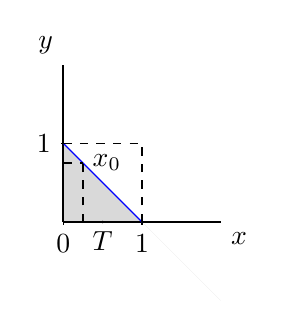
\begin{tikzpicture}
	\fill[color=gray!30]
(0,0) -- (0,1)
-- plot [domain=1:2] (\x,-\x+1)
-- (1,0) -- cycle;
		\draw[thick] (0,0) -- (2,0) node[anchor=north west] {$x$};
		\draw[thick] (0,0) -- (0,2) node[anchor=south east] {$y$};
		\foreach \x in {0,1}
   \draw (\x cm,1pt) -- (\x cm,-1pt) node[anchor=north] {$\x$};
    \foreach \y in {1}
    \draw (1pt,\y cm) -- (-1pt,\y cm) node[anchor=east] {$\y$};
		\draw [blue](0,1) -- (1,0);
		\draw [dashed](0,1) -- (1,1);
		\draw [dashed](1,0) -- (1,1);
		\draw [dashed](0.25,0) -- (0.25,0.75) node[anchor=west] {$x_0$};
		\draw [dashed](0,0.75) -- (0.25,0.75);
		\fill (0.5,0) circle (0.5pt)node[anchor=north] {$T$};
	\end{tikzpicture}
	\end{center}
	\end{figura}
	Calcular la integral de $\xfunction{f}{T}{\R}{(x,y)\to x}$\\\\
	
	$\integral{}{T}xdxdy=\integral{}{T}f(x,y)dxdy=\integral{}{[0,1]\times[0,1]}\overline{f}(x,y)dxdy\overset{\mathrm{Fubini}}= \integral{1}{0}\left(\integral{1}{0}\overline{f}(x,y)dy\right)dx$\\
	Tenemos:\\
	$\integral{1}{0}\overline{f}_{x_0}=\integral{1-x_0}{0}\underset{f(x_0,y)}{\underset{\shortparallel}{\overline{f}_{x_0}}}  + \integral{1}{1-x_0}\underset{0}{\underset{\shortparallel}{\overline{f}_{x_0}}}=\integral{1-x_0}{0}f(x_0,y)dy\implies \integral{}{T}f(x,y)dxdy=\\
	=\integral{1}{0}\left(\integral{1-x}{0}f(x,y)dy\right)dx=\integral{1}{0}\left(\integral{1-x}{0}xdy\right)dx=\integral{1}{0}x(1-x)dx=\left.\dfrac{x^2}{2}-\dfrac{x^3}{3}\right]^1_0=\dfrac{1}{6}$
	\end{ejem}
	\ \\
	\begin{ejem} \ 
	\begin{figura}\ 
	\begin{center}
	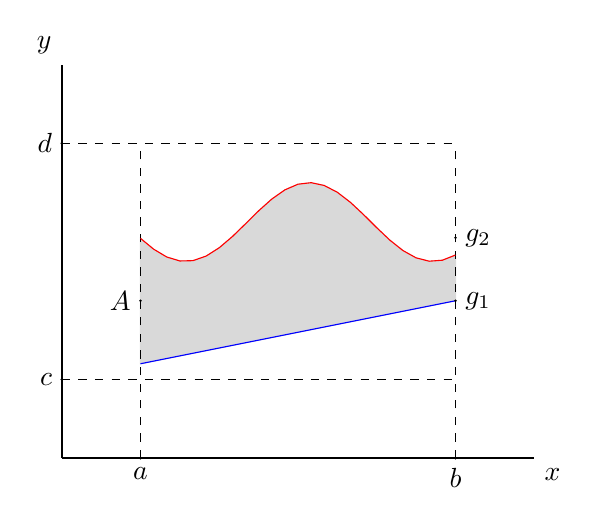
\begin{tikzpicture}
	\filldraw[gray!30] plot [domain=1:5] ({\x},{3 + (1/2)*cos(2*\x r)})
-- plot [domain=5:1] ({\x},{1+0.2*\x})
-- cycle;
		\draw[thick](0,0) -- (6,0) node[anchor=north west] {$x$};
		\draw[thick] (0,0) -- (0,5) node[anchor=south east] {$y$};
		\draw [dashed](0,1) -- (5,1);
		\draw [dashed](0,4) -- (5,4);
		\draw [dashed](1,0) -- (1,4);
		\draw [dashed](5,0) -- (5,4);
		
		
		\draw[domain=1:5,variable=\x,blue] plot ({\x},{1+0.2*\x});
		\draw[domain=1:5,variable=\x,red] plot ({\x},{3 + (1/2)*cos(2*\x r)});
		
		
		\fill (1,0) circle (0.5pt)node[anchor=north] {$a$};
		\fill (5,0) circle (0.5pt)node[anchor=north] {$b$};
		\fill (0,1) circle (0.5pt)node[anchor=east] {$c$};
		\fill (0,4) circle (0.5pt)node[anchor=east] {$d$};
		\fill (1,2) circle (0.5pt)node[anchor=east] {$A$};
		\fill (5,2) circle (0.5pt)node[anchor=west] {$g_1$};
		\fill (5,2.8) circle (0.5pt)node[anchor=west] {$g_2$};
	\end{tikzpicture}
	\end{center}
	\end{figura}
	Sean $\function{g_1,g_2}{[a,b]}{\R}$ continuas, tal que $g_1(x)\leq g_2(x)\ \forall x\in [a,b]$ y sea\\
	$A=\{(x,y)\in\R^2:x\in [a,b],g_1(x)\leq y\leq g_2(x) \}$. Calcular la integral de $\function{f}{A}{\R}$.\\
	$\integral{}{A}f(x,y)dxdy=\integral{}{[a,b]\times[c,d]}\overline{f}(x,y)dxdy=\integral{b}{a}\left(\integral{d}{c}\overline{f}(x,y)dy\right)dx$ \\
	Tenemos que $\integral{d}{c}\overline{f}(x_0,y)dy=\integral{g_1(x_0)}{c}\equals{\overline{f}(x_0,y)dy}{0}+\integral{g_2(x_0)}{g_1(x_0)}\overline{f}(x_0,y)dy+\integral{d}{g_2(x_0)}\equals{\overline{f}(x_0,y)dy}{0}=\\
=\integral{g_2(x_0)}{g_1(x_0)}f(x_0,y)dy$\\
$\implies \integral{}{A}f(x,y)dxdy=\integral{b}{a}\left(\integral{g_2(x)}{g_1(x)}f(x,y)dy\right)dx$
	\end{ejem}
	\newpage
	\begin{ejem} \ 
	\begin{figura}\ 
	\begin{center}
	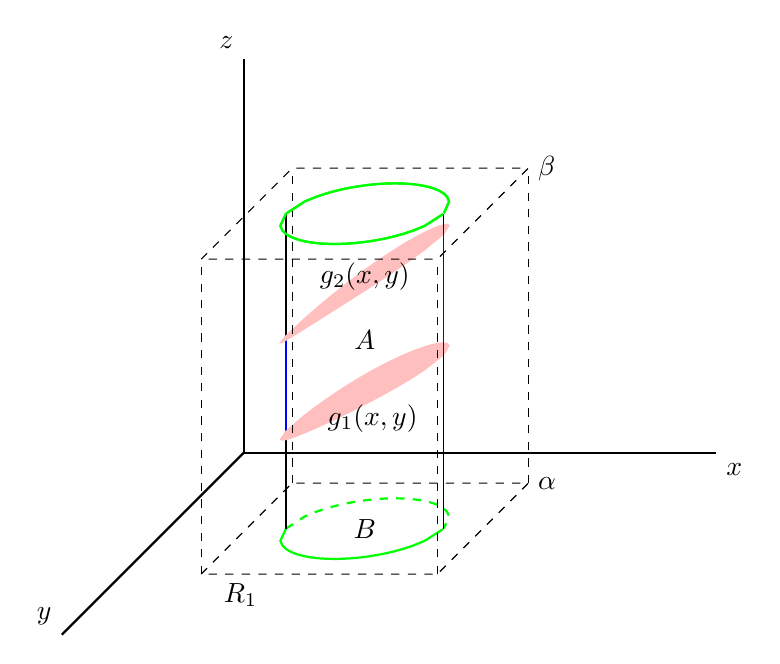
\begin{tikzpicture}
	\draw[thick](0,0,0) -- (6,0,0) node[anchor=north west] {$x$};
	\draw[thick] (0,0,0) -- (0,5,0) node[anchor=south east] {$z$};
	\draw[thick] (0,0,0) -- (0,0,6) node[anchor=south east] {$y$};
	\draw[domain=1.5:3.5,green,thick] plot (\x,0,{(1-(\x-2.5)^2)^(1/2)+2.5});
	\draw[domain=1.5:3.5,dashed,green, thick] plot (\x,0,{-(1-(\x-2.5)^2)^(1/2)+2.5});
	\draw[domain=1.5:3.5,green,thick] plot (\x,4,{(1-(\x-2.5)^2)^(1/2)+2.5});
	\draw[domain=1.5:3.5,green, thick] plot (\x,4,{-(1-(\x-2.5)^2)^(1/2)+2.5});
	
	
	\draw (1.5,0,2.5) -- (1.5,4,2.5);
	\draw [blue](1.5,1.2,2.5) -- (1.5,2.4,2.5);
	
	\filldraw[domain=1.5:3.5,variable=\x,pink] plot (\x,{2*(\x)^(1/2)},{(1-(\x-2.5)^2)^(1/2)+2.5}) plot (\x,{2*(\x)^(1/2)},{-(1-(\x-2.5)^2)^(1/2)+2.5});
	\filldraw[domain=1.5:3.5,variable=\x,pink] plot (\x,{1.5*(\x)^(1/2)-0.6},{(1-(\x-2.5)^2)^(1/2)+2.5}) plot (\x,{1.5*(\x)^(1/2)-0.6},{-(1-(\x-2.5)^2)^(1/2)+2.5});
	
	\draw[dashed]  (1,0,4) -- (1,0,1) -- (4,0,1) -- (4,0,4) -- (1,0,4);
	\draw (1.5,0,4) node[anchor=north] {$R_1$};
	\draw[dashed]  (1,0,1) -- (1,4,1);
	\draw[dashed]  (4,0,1) -- (4,4,1);
	\draw[dashed]  (4,0,4) -- (4,4,4);
	\draw[dashed]  (1,0,4) -- (1,4,4);	
	\draw[dashed]  (1,4,4) -- (1,4,1) -- (4,4,1) -- (4,4,4) -- (1,4,4);
	\draw (3.5,0,2.5) -- (3.5,4,2.5);
	\draw[blue] (3.5,2.2,2.5) -- (3.5,3.8,2.5);
	
	\draw (2.5,3.2,2.5)node {$g_2(x,y)$};
	\draw (2.6,1.4,2.5)node {$g_1(x,y)$};
	\draw (2.5,0,2.5)node {$B$};
	\draw (2.5,2.4,2.5)node {$A$};
	\draw (4,0,1)node[anchor=west]{$\alpha$};
	\draw (4,4,1)node[anchor=west] {$\beta$};
	\draw[domain=1.5:3.5,green,thick] plot (\x,4,{(1-(\x-2.5)^2)^(1/2)+2.5});
	\draw[domain=1.5:3.5,green, thick] plot (\x,4,{-(1-(\x-2.5)^2)^(1/2)+2.5});
	
	\end{tikzpicture}
	\end{center}
	\end{figura}
	Sea $B\subset \R^2$, sean $\function{g_1,g_2}{B}{\R}$ cumpliendo $g_1\leq g_2$. Sea\\
	$A=\{(x,y,z)\in \R^3:(x,y)\in B,g_1(x,y)\leq z\leq g_2(x,y)\}$. Calcular la integral de $\function{f}{A}{\R}$.\\
	$\integral{}{A}f=\underset{R=R_1\times[\alpha,\beta]}{\integral{}{R}\overline{f}}\overset{\mathrm{T.\ Fubini}}= \integral{}{R_1}\left(\integral{\beta}{\alpha}\overline{f}(x,y,z)dz\right)dxdy=\\
	=\integral{}{B}\left(\integral{\beta}{\alpha}\overline{f}(x,y,z)dz\right)dxdy+\equals{\integral{}{R_1\setminus B}\left(\integral{\beta}{\alpha}\overline{f}(x,y,z)dz\right)dxdy}{0}=\\
	=\integral{}{B}\left(\integral{\beta}{\alpha}\overline{f}(x,y,z)dz\right)dxdy=\\
	=\integral{}{B}\left(
	\equals{\integral{g_1(x,y)}{\alpha}\overline{f}(x,y,z)dz}{0} +		
	\integral{g_2(x,y)}{g_1(x,y)}\overline{f}(x,y,z)dz +
	\equals{\integral{\beta}{\alpha}\overline{f}(x,y,z)dz}{0}\right)dxdy=\\
	=\boxed{\integral{}{B}\left(\integral{g_2(x,y)}{g_1(x,y)}\overline{f}(x,y,z)dz\right)dxdy}$
	\end{ejem}
	\newpage
	\begin{ejem} Volumen de revolución de la gráfica de una función $f$ al girarla sobre el eje $OX$.\\
	\begin{figura}\ \\
		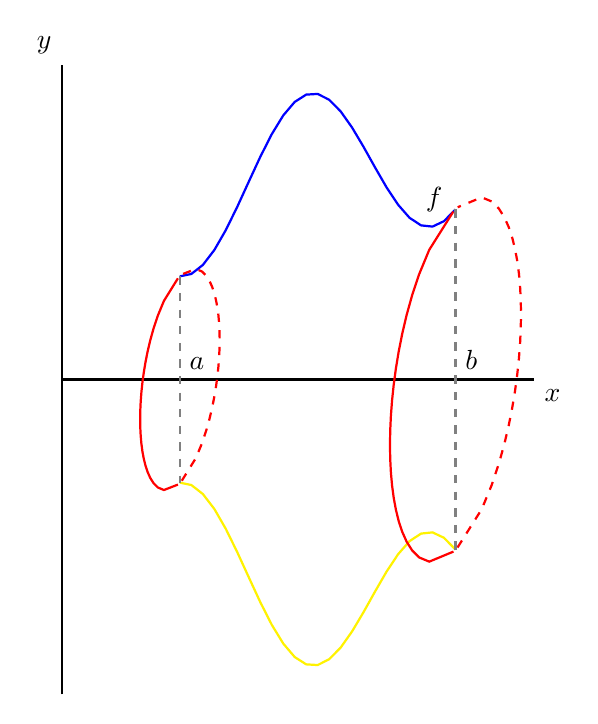
\begin{tikzpicture}
	\draw[thick](0,0,0) -- (6,0,0) node[anchor=north west] {$x$};
	\draw[thick] (0,-4,0) -- (0,4,0) node[anchor=south east] {$y$};	
	\draw[domain=1.5:5,blue,thick] plot (\x,{2+0.2*\x+cos(2*\x r)},0);
\draw[domain=1.5:5,yellow,thick] plot (\x,{-2-0.2*\x-cos(2*\x r)},0);	
	\draw[red,thick,variable=\y,domain=-1.31:1.31] plot (1.5,\y,{(1.72-(\y*\y))^(1/2)});
	\draw[dashed,red,thick,variable=\y,domain=-1.31:1.31] plot (1.5,\y,{-(1.72-(\y*\y))^(1/2)});

	\draw[red,thick,variable=\y,domain=-2.16:2.16] plot (5,\y,{(4.67-(\y*\y))^(1/2)});
	\draw[dashed,red,thick,variable=\y,domain=-2.16:2.16] plot (5,\y,{-(4.67-(\y*\y))^(1/2)});
	\draw[dashed,gray,thick] (1.5,1.31,0) -- (1.5,-1.31,0);
	\draw[dashed,gray,thick] (5,2.16,0) -- (5,-2.16,0);
	\draw (5,0,0) node[anchor=south west] {$b$};
	\draw (1.5,0,0) node[anchor=south west] {$a$};
	\draw (4.5,2,0) node[anchor=south west] {$f$};
	\end{tikzpicture}
	\end{figura}
	\ \\ Volumen$(V)=\integral{b}{a}$Área$(V_x)dx=\integral{b}{a}\pi f(x)^2dx=\pi\integral{b}{a}f(x)^2dx$
	\end{ejem} %Teorema de Fubini
	\chapter{Teorema del cambio de variables}
\section{Teorema del cambio de variables}
\begin{teor} Teorema del cambio de variable.\\
Sean $A$, $B\subset\R^n$, abiertos y medibles-Jordan, y sea $\xfunction{g}{B}{A}{\ \ \ s\longrightarrow x}$ $C^1$-difeomorfismo. Entonces:
\[\integral{}{A}f(x)dx=\integral{}{B}f(g(s))|\det g'(s)|ds\]
Además $\exists m,M>0\talque m\leq|\det g'(s)|\leq M\ \forall s\in B$
\begin{nota} $g$ es $C^1$-difeormorfismo$\iff\det(g'(s)\neq 0)\ \forall s\in B$.\end{nota}
\end{teor}

\section{Coordenadas polares}

\begin{proposicion} Una aplicación del \textit{Teorema del cambio de variables} es la evaluación de integrales por medio de las coordenadas polares. Tomamos la función que pasa de coordenadas polares a rectangulares como $g(r,\theta)=(r\sen\theta,r\cos\theta)$ definida en $\{(r\theta)\talque r>0, 0<\theta<2\pi\}$. El determinante jacobiano viene dado por:
\[J_g(r,\theta)=\left|\begin{matrix}\cos\theta & -r\cos\theta \\ \sen\theta & r\cos\theta\end{matrix}\right|=r\cos^2\theta + r\sen^2\theta=r\]
\end{proposicion}

\begin{ejem} Sea $B=\{(x,y)\in\R^2\talque 1\leq x^2+y^2\leq 2\}$, calcula $\integral{}{B}\dfrac{1}{(x^2+y^2)^3}$.\\
Tenemos que $B$ es la imagen de $A=\{(r,\theta)\talque 0<\theta<2\pi, 1<r<2\}$ bajo la transformación de coordenadas polares. Entonces tenemos:
\[\integral{}{B}\dfrac{1}{(x^2+y^2)^3}=\integral{}{A}\dfrac{1}{r^3}|J_g|drd\theta=\integral{}{A}\dfrac{1}{r^3}rdrd\theta=\integral{}{A}\dfrac{1}{r^2}drd\theta=\integral{2\pi}{0}\integral{2}{1}\dfrac{1}{r^2}drd\theta=\dfrac{1}{2}\integral{2\pi}{0}d\theta=\pi\]
\end{ejem}

\section{Coordenadas esféricas} 
\begin{proposicion} Otra aplicación del \textit{Teorema del cambio de variables} es la aplicación de coordenadas esféricas. Sea $g(r,\varphi,\theta)=(r\sen\varphi\cos\theta,r\sen\varphi\sen\theta, r\cos\varphi)$ definida en $\{(r,\varphi,\theta)\talque r>0, 0<\theta<2\pi, 0<\varphi<\pi\}$ con determinante jacobiano:
\[J_g(r,\varphi,\theta)=\left|\begin{matrix}\sen\varphi\cos\theta & r\cos\varphi\cos\theta & -r\sen\varphi\sen\theta \\ \sen\varphi\sen\theta & r\cos\varphi\sen\theta & r\sen\varphi\cos\theta\\ \cos\varphi & -r\sen\varphi & 0\end{matrix}\right|=r^2\sen\varphi\]
\end{proposicion}

\begin{ejem} Integra la función $f(x,y,z)=x^2+y^2+z^2$ sobre el conjunto\\
$B=\{(x,y,z)\talque x^2+y^2+z^2<1\}$.\\
Tenemos que $B$ es la imagen de $A=\{(r,\varphi,\theta)\talque 0<r<1, 0<\theta<2\pi,0<\varphi<\pi\}$. Por tanto:
\[\integral{}{B}(x^2+y^2+z^2)dxdydz=\integral{}{A}r^2|J_g|drd\varphi d\theta=\integral{}{A}r^2r^2\sen\varphi drd\varphi d\theta=\]\[=\integral{2\pi}{0}\integral{\pi}{0}\integral{1}{0}r^4\sen\varphi drd\varphi d\theta=\integral{2\pi}{0}\integral{\pi}{0}\dfrac{\sen\varphi}{5}d\varphi d\theta=\dfrac{2}{5}\integral{2\pi}{0}d\theta=\dfrac{4}{5}\pi\]
\end{ejem}

\section{Coordenadas cilíndricas} 
\begin{proposicion} Por último veamos la aplicación de las coordenadas cilíndricas. La transformación adecuada es$g(r,\theta,z)=(r\cos\theta,r\sen\theta, z)$ definida en $\{(r,\theta,z)\talque r>0, 0<\theta<2\pi\}$ con determinante jacobiano:
\[J_g(r,\theta,z)=\left|\begin{matrix}\cos\theta & -r sen\theta & 0 \\ \sen\theta & r\cos\theta & 0\\ 0 & 0 & 1\end{matrix}\right|=r\]
\end{proposicion}

\begin{ejem} Integra la función $f(x,y,z)=z\e^{-x^2-y^2}$ sobre la región\\
$R=\{(x,y,z)\talque x^2+y^2\leq1,0\leq z\leq1\}$.\\
Tenemos que $R$ es la imagen de $A=\{(r,\theta,z)\talque 0<r<1, 0<\theta<2\pi,0<z<1\}$. Por tanto:
\[\integral{}{R}z\e^{-x^2-y^2}dxdydz=\integral{}{A}z\e^{-r^2}|J_g|drd\theta dz=\integral{1}{0}\integral{2\pi}{0}\integral{1}{0}z\e^{-r^2}rdrd\theta dz=\]\[=-\dfrac{1}{2}\integral{1}{0}\integral{2\pi}{0}z(e^{-1}-1)d\theta dz=-\pi(e^{-1}-1)\integral{1}{0}zdz=\dfrac{\pi}{2}(1-e^{-1})\]
\end{ejem} %Teorema de cambio de variables
	\chapter{Integrales impropias}	
\section{Integrales impropias}
\begin{defi} Integrales impropias.\\
Sea $\function{f}{\R^n}{\R}$ con $f\geq 0$, supongamos que $\forall k\in N,\ f$ es integrable y acotada en $[-k,k]^n$.\\
Diremos que $f$ es integrable en $\R^n$ si $\exists\limite{}{k\to +\infty}\integral{}{[-k,k]^n}f\ (\in\R)$ y en ese caso, tenemos que $\integral{}{\R^n}f=\limite{}{k\to +\infty}\integral{}{[-k,k]^n}f$.
\end{defi}

\begin{defi} Sea $\sucesionelement{A_n}{n}$ usa sucesión de conjuntos medibles-Jordan en $\R^n$, diremos que es \textbf{exhaustiva} si $\forall k\in\N\ \exists m_k\in\N\talque[-k,k]\subset A_{m_k}$
\end{defi}

\begin{proposicion} Sea $\function{f}{\R^n}{\R}$, $f\geq 0$ y $f$ integrable en $[-k,k]^n\ \forall k\in\N$, son equivalentes:
\begin{enumerate}[i)]
\item $f$ es integrable en $\R^n$
\item Para cada sucesión $\sucesionelement{A_n}{n}$ exhaustiva, existe $\limite{}{\ntiende}\integral{}{A_n}f$
\item $\exists \sucesionelement{A_n}{n}$ exhaustiva de manera que $\exists\ \lim\integral{}{A_n}f$. Además, en este caso, tenemos:
$\integral{}{\R^n}f=\lim\integral{}{A_n}f$ para cualquier función exhaustiva  $\sucesionelement{A_n}{n}$.
\end{enumerate}
\begin{proof}\ 
\begin{itemize}
\item $i)\implies ii)$\\
Dado $k\in\N$, $A_k$ medible-Jordan $\implies A_k$ acotado $\implies\exists R>0\talque A_k\subset B(0,R)\implies\\\implies\integral{}{A_k}f\leq\integral{}{B(0,R)}f\leq\integral{}{\R^n}f$. Por tanto $\integral{}{\R^n}f$ es cota superior de $\sucesionelement{\integral{}{A_k}f}{k}$.\\
Sea $\sucesionelement{A_n}{n}$ exhaustiva. La sucesión $\sucesionelement{\integral{}{A_n}f}{n}$ es monótona no decreciente (Recordemos $f\geq 0$). Ahora, dado $n\in\N$, $\exists k_0\in\N\talque A_n\subset[-k_0,k_0]^n$.\\ Por tanto: $\integral{}{A_n}f\leq  \integral{}{[-k_0,k_0]^n}f\leq \limite{}{\ntiende}\integral{}{[-k_0,k_0]^n}f=\integral{}{\R^n}f$
\item $ii)\implies iii)$ Evidente.
\item $iii)\implies i)$\\
Supongamos $\sucesionelement{A_n}{n}$ exhaustiva tal que $\exists\limite{}{\ntiende}\integral{}{A_n}f$.\\
Veamos que $\integral{}{[-k,k]^n}$ es convergente creciente y está acotada superiormente.\\
$\forall k\in\N\ \exists m_k\in\N\talque[-k,k]^n\subset A_{m_k}$. Por tanto $\integral{}{[-k,k]}f\leq \integral{}{A_{m_k}}\leq \limite{}{\ntiende}\integral{}{A_n}f$
\end{itemize}
\end{proof}
\end{proposicion}

\begin{corolario} \underline{Propiedades elementales de la integral}.
\begin{enumerate}[1)]
\item Sean $\function{f,g}{\R^n}{\R},\ f,g\geq 0$:
\[\integral{}{\R^n}f+g=\integral{}{\R^n}f+\integral{}{\R^n}g\]
\item Sean $\function{f}{\R^n}{\R},\ f\geq 0$ y $\alpha\geq 0$: 
\[\integral{}{\R^n}\alpha f=\alpha\integral{}{\R^n}f\]
\item Sean $\function{f,g}{\R^n}{\R},\ 0\leq f\leq g$:
\[\integral{}{\R^n}f\leq\integral{}{\R^n}g\]
\item Sean $A,B\subset\R^n$ con $A\cap B$ medida nula:
\[\integral{}{A\cup B}f=\integral{}{A}f+\integral{}{B}f\]
\item Sean $f,g$ continuas en casi todo punto y acotadas
\begin{itemize}
\item Si $0\leq f\leq g$, entonces: 
$g \mathrm{\ es\ integrable\ en\ }\R^n\implies f \mathrm{\ es\ integrable\ en\ }\R^n$
\item $\integral{}{\R^n}g <+\infty\implies \integral{}{\R^n}f <+\infty$
\item $\integral{}{\R^n}f \leq \integral{}{\R^n}g$
\end{itemize} 
\item Sea $A\subset\R^n$, entonces:
\[\integral{}{A}f=\integral{}{\R^n}f\chi_A\]
\end{enumerate}
\end{corolario}

\begin{defi} Sea $\function{f}{\R^n}{\R}$, $f\geq 0$, $f$ no acotado.\\
Para cada $M>0$ definimos $\xfunction{f_M}{\R^n}{\R}{x\to\doubleleft{f(x)\mathrm{\ si\ }f(x)\leq M}{0\mathrm{\ si\ }f(x)>M}}$\\
Es claro que $0\leq f_M$ y $f_M$ es acotada. Supongamos que $f_M$ es integrable en $\R^n\ \forall M>0$ y que $\exists\limite{\integral{}{\R^n}f_M}{M\to\infty}$. Entonces decimos que $f$ es integrable en $\R^n$ y tenemos que\\
$\integral{}{\R^n}f=\limite{}{M\to\infty}\integral{}{\R^n}f_M$.
\end{defi}

\begin{defi} Definamos ahora integración pero sin necesidad de que $f$ sea positiva.\\
Sea $\function{f}{\R^n}{\R}$, llamamos $f^+(x)$ y $f^-(x)$ a las funciones:
\[f^+(x)=\doubleleft{f(x)\mathrm{\ si\ }f(x)\geq 0}{\ \ \ \ \ 0\mathrm{\ si\ }f(x)< 0}\]
\[f^-(x)=\doubleleft{-f(x)\mathrm{\ si\ }f(x)\leq 0}{\ \ \ \ \ \ \ 0\mathrm{\ si\ }f(x)> 0}\]
Entonces $f(x)=f^+(x)-f^-(x)$. Decimos que $f$ es integrable si $f^+$ y $f^-$ lo son, y en este caso tenemos $\integral{}{\R^n}f=\integral{}{\R^n}f^+-\integral{}{\R^n}f^-$
\end{defi}

\begin{proposicion} $f$ es integrable $\iff f$ es continua en casi todo punto y $|f|$ es integrable.
\begin{proof}\ 
\begin{itemize}
\item $(\implies)$\\
$f$ integrable $\implies f$ continua en casi todo punto y $f^+,\ f^-$ integrables $\ximplies{\mathrm{por\ prop.\ elem.}}{} f^+ + f^-=|f|$ es integrable.
\item $(\impliedby)$\\
$\doubleright{0\leq f^+\leq|f|\ximplies{\mathrm{por\ prop.\ elem.}}{} f^+\mathrm{\ es\ integrable}}{0\leq f^-\leq|f|\ximplies{\mathrm{por\ prop.\ elem.}}{} f^-\mathrm{\ es\ integrable}}\implies f$ es integrable.
\end{itemize}
\end{proof}
\end{proposicion}


\begin{observacion} Veamos que se cumple la propiedad de linealidad.\\
Sean  $\function{f,g}{\R^n}{\R}$ integrables $\implies f+g$ es integrable y $\integral{}{\R^n}f+g=\integral{}{\R^n}f+\integral{}{\R^n}g$
\begin{proof}\ \\
Tenemos que $f+g$ es continua en casi todo punto. Además $|f+g|\leq|f|+|g|\implies|f+g|$ integrables$\implies f+g$ integrables.\\
Ahora veamos que $\integral{}{\R^n}f+g=\integral{}{\R^n}f+\integral{}{\R^n}g$.\\
$f+g = (f+g)^+-(f+g)^-=f^+-f^-+g^+-g^-\implies (f+g)^++f^-+g^-=(f+g)^-+f^++g^+$\\
Tenemos ahora que $\integral{}{\R^n}(f+g)^++\integral{}{\R^n}f^-+\integral{}{\R^n}g^-=\integral{}{\R^n}f^++\integral{}{\R^n}g^++\integral{}{\R^n}(f+g)^-\implies\\\implies \integral{}{\R^n}(f+g)^+-\integral{}{\R^n}(f+g)^-=\integral{}{\R^n}f^+-\integral{}{\R^n}f^-+\integral{}{\R^n}g^+-\integral{}{\R^n}g^-\implies\\\implies\integral{}{\R^n}f+g=\integral{}{\R^n}f+\integral{}{\R^n}g$
\end{proof}
\end{observacion}

\begin{defi} Sea $A\subset\R^n$ y sean $\sucesionelement{f_n}{n}$ y $f$ funciones reales definidas en $A$, diremos que $\sucesionelement{f_n}{n}$ \underline{converge uniformemente} a $f$ en $A$ si:
\[\forall\varepsilon>0\ \exists n_\varepsilon\in\N\talque\forall n\geq n_\varepsilon\ |f_n(x)-f(x)|<\varepsilon\ \forall x\in A\]
Nótese que la definición de convergencia puntual es:
\[\forall x\in A,\ \forall\varepsilon>0\ \exists n_{\varepsilon,x}\in\N\talque\forall n\geq n_{\varepsilon,x}\ |f_n(x)-f(x)|<\varepsilon\]
Luego es claro ver que convergencia uniforme $\implies$ convergencia puntual.
\end{defi}

\begin{proposicion} Si $\{f_n\}\limited f$ uniformemente en $A$ y $f_n$ continua en $A\ \forall n\in\N$, entonces $f$ es continua en $A$.
\begin{observacion}
\end{observacion} Como consecuencia de la proposición, $x^n$ no converge uniformemente en $[0,1]$ ya que $x^n$ es continua en $[0,1]\ \forall n\in\N$ pero el límite no lo es.
\end{proposicion}

\begin{teor} Sea $A\subset\R^n$ medible-Jordan, $\sucesionelement{f_n}{n}$ y $f$ funciones reales definidas en $A$. Supongamos que $\sucesionelement{f_n}{n}$ converge uniformemente a $f$ en $A$ y que $f_n$ es integrable $\forall n\in\N$. Entonces $f$ es integrable y:
\[\limite{}{\ntiende}\integral{}{A}f_n=\integral{}{A}f\]
\end{teor}

\begin{teor} Sea $\function{f}{[a,b]\times[c,d]}{\R}$ continua, definimos:\\
$F(x)=\integral{d}{c}f(x,y)dy$ (es decir $\function{F}{[a,b]}{\R}$).\\
Entonces $F$ es continua en $[a,b]$.
\begin{nota} Podemos sustituir $\function{f}{[a,b]\times[c,d]}{\R}$ por $\function{f}{K\times K_0}{\R}$ con $K\in \R^m$ compacto y medible-Jordan y $K_0\in\R^n$ compacto.
\end{nota}
\begin{proof} \ \\
Supongamos que se cumple la hipótesis. ¿$F$ es continua en $[a,b]$?\\
Sea $\sucesion{x}{n}\subset[a,b]\talque x_n\limited x_0$ comprobemos que $F(x_n)\limited F(x_0)$.\\
$\limite{F(x_n)}{\ntiende}=\limite{}{}$
\end{proof}
\end{teor} %Integrales impropias
	%-----------------
	%---Falta:
	% Ejemplos cambio de variable
	%-----------------	
	
	%\chapter{Longitud de curvas e integrales de línea}
	%\chapter{Teorema de Green}
	%\chapter{Área de una superficie e integrales sobre una superficie}
	%\chapter{Teoremas de Stokes y Gauss}
	

%---------------------------------------
	%Aquí empiezan los apéndices
	\appendix\chapter{Cálculo de límites} \label{App:AppendixA}
	
	Veamos las siguientes propiedades y consejos para calcular límites.
	\begin{enumerate}[1)]
	\item Uso de las propiedades algebraicas y de composición de funciones continuas.
	\begin{ejem} $\limite{}{(x,y)\to(0,0)}\dfrac{2\sen x\tan y}{xy}=\limite{}{(x,y)\to(0,0)}\dfrac{2\sen x}{x}\dfrac{\tan y}{y}$, tenemos ahora que:\\
	$\doubleleft{\limite{}{(x,y)\to(0,0)}\dfrac{2\sen x}{x}\overset{\mathrm{L'H\hat{o}pital}}=\limite{}{(x,y)\to(0,0)}\dfrac{2\cos x}{1}=2}{\limite{}{(x,y)\to(0,0)}\dfrac{\tan y}{y}\overset{\mathrm{L'H\hat{o}pital}}=\limite{}{(x,y)\to(0,0)}\dfrac{1}{\cos^2y}=\dfrac{1}{1}=1}$\\
	Luego $\limite{}{(x,y)\to(0,0)}\dfrac{2\sen x}{x}\dfrac{\tan y}{y}=2\cdot1=2$
	\end{ejem}
	\item Uso de la siguiente igualdad: $\limite{}{(x,y)\to(a,b)}f(x,y)=\limite{}{(h,k)\to(0,0)}f(a+h,b+k)$.
	\item $\limite{}{(x,y)\to(a,b)}f(x,y)=L\iff \limite{}{(x,y)\to(a,b)}(f(x,y)-L)=0\iff \limite{}{(x,y)\to(a,b)}|f(x,y)-L|=0$.
	\item Calcular los límites a través de rectas.
	\begin{ejem} Calculemos $\limite{}{(x,y)\to(0,0)}\dfrac{xy}{x^2+y^2}$.\\
	Sea $y=\lambda x$, tenemos que $\limite{}{(x,y)\to(0,0)}f(x,y)=\limite{}{x\to 0}f(x,\lambda x)=\limite{}{x\to 0}\dfrac{x(\lambda x)}{x^2+(\lambda x)^2}=\\
	=\limite{}{x\to 0}\dfrac{\lambda x^2}{x^2(1+\lambda^2)}=\dfrac{\lambda}{1+\lambda^2}$. Por tanto, como el límite depende de $\lambda\implies$ no existe el límite.
	\end{ejem}
	\item Hallando los límites iterados.
	\newpage
	\begin{ejem} Calculemos $\limite{}{(x,y)\to(0,0)}\dfrac{x-y}{x+y}$.\\
	$\doubleright{\limite{}{y\to 0}\left(\limite{}{x\to0}\dfrac{x-y}{x+y}\right)=\limite{}{x\to 0}\dfrac{x}{x}=1}{\limite{}{x\to 0}\left(\limite{}{y\to0}\dfrac{x-y}{x+y}\right)=\limite{}{y\to 0}\dfrac{-y}{y}=-1}\implies 1\neq -1\implies\nexists\limite{}{(x,y)\to(0,0)}\dfrac{x-y}{x+y}$.
	\end{ejem}
	\item Uso del \textit{criterio de compresión}:\\
	Si $g(x,y)\leq f(x,y)\leq h(x,y)\ \forall(x,y)\in B((a,b),r)\setminus\{(a,b)\}$ para un cierto $r$, entonces, si $\limite{}{(x,y)\to(a,b)}g(x,y)=\limite{}{(x,y)\to(a,b)}h(x,y)=L\implies\exists\limite{}{(x,y)\to(a,b)}f(x,y)=L$.
	\begin{ejem} Calculemos $\limite{}{(x,y)\to(0,0)}\dfrac{(x+y)\sen y}{y(x^2+2)}$.\\
	$0\leq\left|\dfrac{(x+y)\sen y}{y(x^2+2)}\right|\leq \left|\dfrac{\sen y}{y}\right|\left|\dfrac{x+y}{x^2+2}\right|\leq 1\left|\dfrac{x+y}{x^2+2}\right|\leq \dfrac{1}{2}|x+y|\leq\dfrac{1}{2}(|x|+|y|)$. Como $\limite{}{(x,y)\to(0,0)}\dfrac{1}{2}(|x|+|y|)=0\ximplies{\mathrm{C.\ compresi\acute{o}n}}{}\exists \limite{}{(x,y)\to(0,0)}\dfrac{(x+y)\sen y}{y(x^2+2)}=0$.
	\end{ejem}
	\item Cuando el límite es del tipo $(x,y)\to(0,0)$, podemos hacer uso del cambio de variable a polares.
	\begin{ejem} Calculemos $\limite{}{(x,y)\to(0,0)}\dfrac{xy}{\sqrt{x^2+y^2}}$.\\
	$\limite{}{r\to0^+}f(r\cos\theta,r\sin\theta)=\limite{}{r\to0^+}\dfrac{(r\cos\theta)(r\sin\theta)}{\sqrt{r^2\cos^2\theta+r^2\sin^2\theta}}=\limite{}{r\to0^+}\dfrac{r^2\cos\theta\sin\theta}{r}=\limite{}{r\to0^+}r\cos\theta\sin\theta=\\
	=0$. Veamos que la convergencia es uniforme en $\theta\in[0,2\pi]$:\\
	$0\leq |f(r\cos\theta,r\sin\theta)|=r|\cos\theta\sin\theta|\leq r$. Así, dado $\varepsilon>0,\ \exists\delta=\varepsilon>0$ tal que si $0<r<\delta$ entonces $|f(r\cos\theta,r\sin\theta)|\leq r<\delta=\varepsilon\ \forall\theta\in[0,2\pi]$.
	\end{ejem}
	\begin{nota}Si el límite no es uniforme en $\theta$, el límite de partida puede no existir.\end{nota}
	\end{enumerate}
	
	
	\chapter{Repaso de aplicaciones lineales} \label{App:AppendixB}	
	
	\begin{proposicion} Si $E$ y $F$ son espacios normados y $\function{L}{E}{F}$ es una aplicación lineal, entonces son equivalentes:
	\begin{enumerate}[a)]
	\item $L$ es continua en $E$
	\item $L$ es continua en $0$.
	\item $\exists M>0	\talque \norm{L(x)}_F\leq M\norm{x}_E\ \forall x\in E$
	\item $L(B_E)$ es acotado en $F$ (donde $B_E$ es la bola de centro el origen y radio $1$).
	\end{enumerate}
	\end{proposicion}
	
	\begin{observacion}
	En el cojunto $\mathfrak{L}(E,F)$ de aplicaciones lineales y continuas podemos definir una norma de la siguiente manera. Si $L\in\mathfrak{L}(E,F)$, se define $\norm{L}=\stackbin[\norm{x}_E\leq 1]{}\sup\norm{L(x)}_F$\\
	Se comprueba que $\stackbin[\norm{x}_E\leq 1]{}\sup\norm{L(x)}_F=\stackbin[\norm{x}_E]{}\sup\norm{L(x)}_F=\inf\{M>0\colon \norm{L(x)}_F\leq M\norm{x}_E\\ \forall x\in E\}$. Como consecuencia de lo anterior, si $E$ es de dimensión finita, toda aplicación lineal $\function{L}{E}{F}$ es continua.
	\end{observacion}
	
	\begin{observacion} Si $\function{L}{\R^n}{\R}$ y para cada $1\leq i \leq n$ llamamos $\alpha_i=L(e_i)$ tenemos que $\norm{L(e)}=\norm{\alpha_1,\alpha_2,...,\alpha_n}_2=\sqrt{\alpha_1^2+\alpha_2^2+...+\alpha_n^2}$\\	
	Toda aplicación lineal $\function{L}{\R^n}{\R^m}$ tiene una matriz asociada $A_{L\ m\times n}$ donde\\ $L(h)=L(h_1,h_2,...,h_n)=(u_1,u_2,...,u_n)$ si solo si $A_L\begin{pmatrix}
  h_1 \\ \vdots \\ h_n  \end{pmatrix}=\begin{pmatrix}  u_1 \\ \vdots \\ u_n  \end{pmatrix}$.\\
  Sea $L=(L_1,L_2,...,L_n)\talque \function{L_i}{\R^n}{\R}$, $A_L=\stackbin[1\leq j\leq n]{}{\stackbin[1\leq i\leq n]{}{(a_{ij})}}$ donde $a_{ij}=L_i(e_j)$.\\
  Ahora, sea $\R^n\xrightarrow{L}\R^m\xrightarrow{S}\R^k$ si $L$ y $S$ son lineales, entonces: $A_{S\circ L}=A_S\cdot A_L$
	\end{observacion}
	
	\chapter{Repaso de formas cuadráticas} \label{App:AppendixC}

\begin{defi} Dada una matriz $n\times n$, $A=(\alpha_{ij})^n_{i,j=1}$, se llama forma cuadrática asociada a la matriz $A$ a la aplicación $\xfunction{Q_A}{\R^n}{\R}{\ \ \ \ h\ \longrightarrow\ hAh^t}$. Es decir $Q_A(h)=\stackbin[i,j=1]{n}\sum h_ih_j\alpha_{ij}$.
\end{defi}

\begin{defi} Sea $Q$ una forma cuadrática, la denominamos:
\begin{itemize}
\item Semidefinida positiva si $Q(h)\geq 0\ \forall h\in\R^n\setminus\{0\}$.
\item Semidefinida negativa si $Q(h)\leq 0\ \forall h\in\R^n\setminus\{0\}$.
\item Definida positiva si $Q(h)> 0\ \forall h\in\R^n\setminus\{0\}$.
\item Definida negativa si $Q(h)< 0\ \forall h\in\R^n\setminus\{0\}$.
\item Indefinida si $\exists h,\oversim{h}\in\R^n\talque Q(h)<0<Q(\oversim{h})$.
\end{itemize}
\end{defi}

\begin{proposicion}
Sea $A$ una matriz simétrica y sea $Q_A$ la forma cuadrática asociada a $A$, se tiene que:
\begin{itemize}
\item $Q_A$ es semidefinida positiva $\iff$ sus autovalores son $\geq 0$.
\item $Q_A$ es semidefinida negativa $\iff$ sus autovalores son $\leq 0$.
\item $Q_A$ es definida positiva $\iff$ sus autovalores son $> 0$.
\item $Q_A$ es definida negativa $\iff$ sus autovalores son $< 0$.
\end{itemize}
\end{proposicion}

\begin{proposicion} Criterio de \textit{Sylvester}.\\
Sea $Q$ la matriz cuadrática asociada a la matriz simétrica $A=(a_{ij})^n_{i,j=1}$ y sea $A_k=\\
=\det\begin{pmatrix}a_{11}&\ldots&a_{1k}\\\vdots&\ddots&\vdots\\a_{k1}&\ldots&a_{kk}\end{pmatrix}$ con $k\in \{1,2,...,n\}$. Entonces:
\begin{enumerate}[i)]
\item $Q$ es definida positiva $\iff A_k>0\ \forall k\in \{1,2,...,n\}$.
\item $Q$ es definida negativa $\iff (-1)^kA_k>0\ \forall k\in \{1,2,...,n\}$.
\item $Q$ es semidefinida positiva $\iff A_k\geq 0\ \forall k\in \{1,2,...,n\}$.
\item $Q$ es semidefinida negativa $\iff (-1)^kA_k\geq 0\ \forall k\in \{1,2,...,n\}$.
\item Si $\exists k_0\talque A_{k_0}<0 \implies Q$ es indefinida.
\end{enumerate}
\end{proposicion}

\begin{observacion} Sea $Q(x)=\stackbin[i,j=1]{n}\sum x_ix_ja_{ij}\ \forall x\in\R^n$:\\
Si $Q(x)>0\implies Q(tx)=t^2(Q(x))>0\ \forall t\in\R\setminus \{0\}$.\\
Si $Q(x)<0\implies Q(tx)=t^2(Q(x))<0\ \forall t\in\R\setminus \{0\}$.
\end{observacion} %Apéndices

\end{document}